\documentclass[]{nsm-thesis}
% options:
% [germanthesis] - Thesis is written in German
% [plainunnumbered] - Don't print numbers on plain pages
% [earlydraft] - Settings for quick draft printouts
% [watermark] - Print current time/date at bottom of each page
% [phdthesis] - switch to PhD thesis style
% [twoside] - double sided
% [cutmargins] - text body fills complete page

% Author name; separate multiple authors with commas.
\author{Mohamed Ben Ahmed}
\birthday{22 July 1997}
\birthplace{Tunisia}

% Title of your thesis.
\title{Entwicklung, Implementierung und Simulation
eines Routing-Algorithmus im Zukunftsfeld
Multi-Domain Operations}

% Choose one of the following lines.
\thesistype{Bachelor Thesis}
%\thesistype{Bachelor Thesis}
%\thesistype{Master's Thesis}
%\thesistype{Diploma Thesis}

% Choose one of the following lines or amend as necessary.
\degreeprogram{Computer Science}
%\degreeprogram{Computational Logic}
%\degreeprogram{Computational Modeling and Simulation}
%\degreeprogram{Distributed Systems Engineering}
%\degreeprogram{Information Systems Engineering}
%\degreeprogram{Media Informatics}

% List of advisors (without academic titles), separated by commas; comment out if not needed.
\advisors{Erika Musterfrau}

% List of referees (without academic titles), separated by commas.
\referees{Christoph Sommer, Jane Doe}


% Define abbreviations used in the thesis here.
\acrodef{WSN}{Wireless Sensor Network}
\acrodef{MANET}{Mobile Ad Hoc Network}
\acrodef{ROI}{Region of Interest}{short-indefinite={an}, long-plural-form={Regions of Interest}}
\acrodef{ADAC}{German Automobile Association}{foreign={Allgemeiner Deutscher Automobilclub}}
\acrodef{CANhashing}[CAN]{Content Addressable Network}{extra={when referring to the distributed hash table}}
\acrodef{CANproto}[CAN]{Controller Area Network}{extra={when referring to the bus protocol}}
\usepackage{longtable}
\usepackage{tikz}
\usepackage{algorithm}
\usepackage{algorithmic}
\usepackage{algpseudocode}
\usetikzlibrary{shapes.geometric, arrows}
\tikzstyle{startstop} = [rectangle, rounded corners, minimum width=1.5cm, minimum height=0.5cm,text centered, draw=black, fill=red!30]
\tikzstyle{process} = [rectangle, minimum width=1.5cm, minimum height=0.5cm, text centered, draw=black, fill=blue!30]
\tikzstyle{decision} = [diamond, minimum width=0.05cm, minimum height=0.025cm, text centered, draw=black, fill=green!30]
\tikzstyle{arrow} = [thick,->,>=stealth]


\begin{document}

\pagenumbering{roman}

\maketitle

\cleardoublepage



\chapter*{Abstract}
\addcontentsline{toc}{chapter}{Abstract}
\begin{otherlanguage*}{american}
The integration of above-water and underwater communication systems is critical for applications such as environmental monitoring and underwater exploration, where the reliability of maritime infrastructure is vital. This study addresses the challenges of bridging above-water and underwater domains, which are impacted by factors such as signal attenuation, high latency, and limited bandwidth. The proposed solution extends the basic Ad-hoc On-demand Distance Vector (AODV) protocol to support seamless communication between these environments. The basic AODV protocol is implemented for above-water communication, while an extended version of AODV is used to facilitate communication between the above-water and underwater subdomains through a gateway. Both protocols are implemented in Python on Raspberry Pi devices, leveraging acoustic modems for underwater data transmission. The system incorporates new message types, such as Relay Request and Relay Reply, to enhance route discovery and optimize network performance. Gateway selection is done by choosing the minimal distance to the underwater node, ensuring efficient routing.

The performance of the system was evaluated through a series of tests, including one-hop and two-hop tests, using metrics such as Packet Delivery Ratio (PDR) and Round Trip Time (RTT). These tests assessed the functionality and efficiency of the routing protocols, both for above-water communication using the basic AODV and for the integration of above-water and underwater domains using the extended AODV protocol. The results showed that while the extended AODV protocol reliably connects the two domains, it introduces additional latency due to the relay process. This research highlights the potential for hybrid communication networks to support critical maritime applications and suggests areas for future improvement, including optimization of the relay mechanism and refinement of gateway selection.


\end{otherlanguage*}


\chapter*{Kurzfassung}
\addcontentsline{toc}{chapter}{Kurzfassung}
\begin{otherlanguage*}{german}
Die Kombination von überwasser- und unterwasserbasierten Kommunikationssystemen ist für Anwendungen wie Umweltüberwachung und Unterwasserforschung von entscheidender Bedeutung. In diesen Bereichen ist eine zuverlässige maritime Infrastruktur unerlässlich. Diese Studie beschäftigt sich mit den Herausforderungen der Verbindung von über- und unterwasserliegenden Bereichen, die durch Probleme wie Signalabschwächung, Kommunikationsverzögerungen und begrenzte Datenkapazität entstehen. Die vorgeschlagene Lösung erweitert das grundlegende Ad-hoc On-demand Distance Vector (AODV)-Protokoll, um eine nahtlose Kommunikation zwischen den verschiedenen Umgebungen zu ermöglichen. Das Standard-AODV-Protokoll wird für die Kommunikation über Wasser genutzt, während eine angepasste Version des AODV-Protokolls eine Verbindung zwischen über- und unterwasser durch ein Gateway ermöglicht. Beide Protokolle wurden mit Python auf Raspberry Pi Geräten implementiert, wobei akustische Modems für die Datenübertragung unter Wasser verwendet werden. Das System fügt neue Nachrichtentypen wie Relay Request und Relay Reply hinzu, um die Routenfindung zu verbessern und die Netzwerkleistung zu optimieren. Bei der Auswahl eines Gateways wird dasjenige ausgewählt, das dem unterwasser Knoten am nächsten ist, um eine effiziente Weiterleitung zu gewährleisten.

Mehrere Tests, darunter Ein-Hop- und Zwei-Hop-Tests, wurden durchgeführt, um die Leistung des Systems zu bewerten. Dabei wurden Metriken wie Round Trip Time (RTT) und Packet Delivery Ratio (PDR) herangezogen. Diese Experimente prüften die Effektivität und Funktionalität der Routing-Protokolle für sowohl die Kommunikation über Wasser mit dem grundlegenden AODV-Protokoll als auch die Integration der über- und unterwasserbasierten Netzwerke mit dem erweiterten AODV-Protokoll. Die Ergebnisse zeigten, dass das erweiterte AODV-Protokoll die beiden Bereiche zuverlässig verbindet, jedoch zusätzliche Latenz aufgrund des Relaismechanismus aufweist. Diese Studie verdeutlicht, wie hybride Kommunikationsnetzwerke wichtige maritime Anwendungen unterstützen können, und weist auf Verbesserungspotentiale hin, wie die Optimierung des Relaismechanismus und die Weiterentwicklung der Gateway-Auswahl.

\end{otherlanguage*}
\acresetall

\cleardoublepage
\tableofcontents


\cleardoublepage
\pagenumbering{arabic}


\chapter{Introduction}
%\chapter{Einleitung}
\label{sec:introduction}
\section{General Motivation}
Over the past 100 years, the ocean has witnessed significant growth in its infrastructure, including the expansion of pipelines and fiber optic cables. Additionally, the shipping industry and port operations have seen considerable development. Modern economies and societies are heavily reliant on this maritime infrastructure. Critical functions such as trade, supply chains, energy, and food security depend on it, which is why it is referred to as critical maritime infrastructure, vital for the functioning of society.\cite{BUEGER2023105772}\\
\\
Given its importance, the protection and security of this infrastructure have become major topics of discussion. Ensuring its resilience and finding rapid solutions in the event of damage are of paramount concern. One approach to addressing these challenges is through the use of Multi-Domain Operations (MDO) and unmanned vehicles, such as Unmanned Underwater Vehicles (UUVs), Unmanned Aerial Vehicles (UAVs), and Unmanned Surface Vehicles (USVs). These technologies enable the integration of operations above and below the water, allowing for the exchange of critical data essential for missions and ensuring the safety of maritime sectors.

\section{Problem Statement}
For successful information exchange between UxVs, a self-organized network is essential. This network allows for seamless data transfer even if one UxV is shut down or damaged, enabling other routes or vehicles to be utilized for data exchange. Without such a system, critical data could be lost, Endangering the mission's success.

One promising approach to facilitate communication across different domains, including above-water and underwater environments, is the Mobile Ad Hoc Network (MANET). This solution supports the creation of a self-organized network without relying on existing infrastructure.

Although MANET is suitable for our needs in a MDO context, it does have limitations, particularly in integrating above-water and underwater communication systems. Above-water communication relies on electromagnetic signal transmission, which offers high data rates and extended ranges between network nodes. In contrast, underwater communication typically employs acoustic signals due to their superior penetration capabilities and greater range. However, these acoustic signals are constrained by low data rates and experience noticeable delays due to the slow propagation speed in water.

Integrating above-water and underwater protocols presents a complex challenge, as it requires bridging technological differences and adapting to the distinct physical properties of each environment.
\section{Proposed Solution}
In General The routing strategies of MANET network protocols can be divided into three categories : reactive, proactive, and hybrid. For the above water communication is based on elctromagnetic signal transmissions . Based on this the following has been established : Ad-hoc On-demand Distance Vector(AODV) and  Dynamic Source Routing (DSR) as a reactive protocol ,Destination Sequenced Distance Vector Routing(DSDV)and Optimized Link State Routing (OLSR) as proactive protocol ,Zone Routing Protocol(ZRP) and Hybrid Wireless Mesh Protocol (HWMP) as hybrid protocol . In this thesis our focus will be on the using  aodv as protcol for above water comunication .As for under water communication UWAODV protcol gonna be used as variante of AODV but instead of above water is going be underwater . As for the integration of these two subdomain  there is no signale system that allow a direct   comunication between the above water subdomain and the under water subdomain , that is why a Gateway (USV) idea was introduce wich is gonna represent as doorway for communication with the nodes under the water if they are the destination that intend to communicate with them but more to that later .

\section{Thesis contribution}
The list of contributions can be summarized as described below:
\begin{itemize}
    \item Implementing AODV protocol with python on different Raspberry pi(Raspi) that going to reprensent different nodes (UAV,USV,UUV).
    \item Implementing  new message type ; Relay Request and Relay Reply wich are crucial for the comunication with under water subdomains nodes through gateway. 
    \item Optimale selecting of Gateway (USV) to tranfer the data from above water subdomain (Radio medium)) to under water water subdomain (Acoustic medium)  
    \item Evaluating the system Ability of sending the data to the destination without any lost by using the packet delivery ratio (PDR).
    \item Using The Latency ,The time required for a data packet to be delivered to the destination,as metric for real-time especially for the underwater subdomain.
\end{itemize}
\section{Structure of the Thesis}

\begin{itemize}
\item Chapter 1: Introduction 
\item Chapter 2: Background
\item Chapter 3: State of Art 
\item Chapter 4: Methods
\item Chapter 5: Concepts of practical Implementation
\item Chapter 6: Practical Setup 
\item Chapter 7: Results and Discussion
\item Chapter 8: Conclusion and Future Work

\end{itemize}

\chapter{Background}
\section{Hardware}
\subsection{UAV}

For this project, a Raspberry Pi is employed  as a communication hop within our underwater network. To protect and secure the device in aquatic environments, the Raspi is housed in a 3D-printed case, designed to fit seamlessly with the SwellPro drone. SwellPro drones are renowned for their robust waterproofing, making them an ideal platform for deploying electronic equipment in water-based operations. The combination of the 3D-printed casing and the drone's waterproof capabilities ensures the durability and functionality of the Raspi, even in challenging marine conditions. This integration allows for reliable underwater communication while leveraging the drone's maneuverability and resilience.
\begin{figure}[h!]
    \centering
    \includegraphics[width=0.65\textwidth]{image/Drohne.JPG}
    \caption{Drone}
    \label{fig:example}
\end{figure}

\subsection{Moritz}
MORITZ is a sophisticated autonomous surface vehicle designed for various testing applications, including autonomous driving, sensor evaluation, and human-machine interfaces. Initially developed by Thyssenkrupp Marine Systems for search-and-rescue missions in particular, to find lost containers and reduce sea traffic hazards, MORITZ has been fitted with a large set of sensors: AIS cameras, RADAR cameras, and 360° cameras.

The vehicle enables seamless integration of data, presenting the users with vital information such as ship tracks, weather data, and vehicle status. MORITZ transforms raw sonar, RADAR, and GPS data through novel algorithms for data fusion into user-friendly visualizations and strives to improve maritime operations.

The system also supports immersive interfaces, like streaming to VR headsets, where operators can interactively navigate and analyze data. MORITZ is designed with the intention of achieving a more advanced yet user-friendly system that integrates multiple sources to help in maritime operations with unparalleled ease.
\begin{figure}[h]
\graphicspath{{/image/}} % Directory path for images
\centering
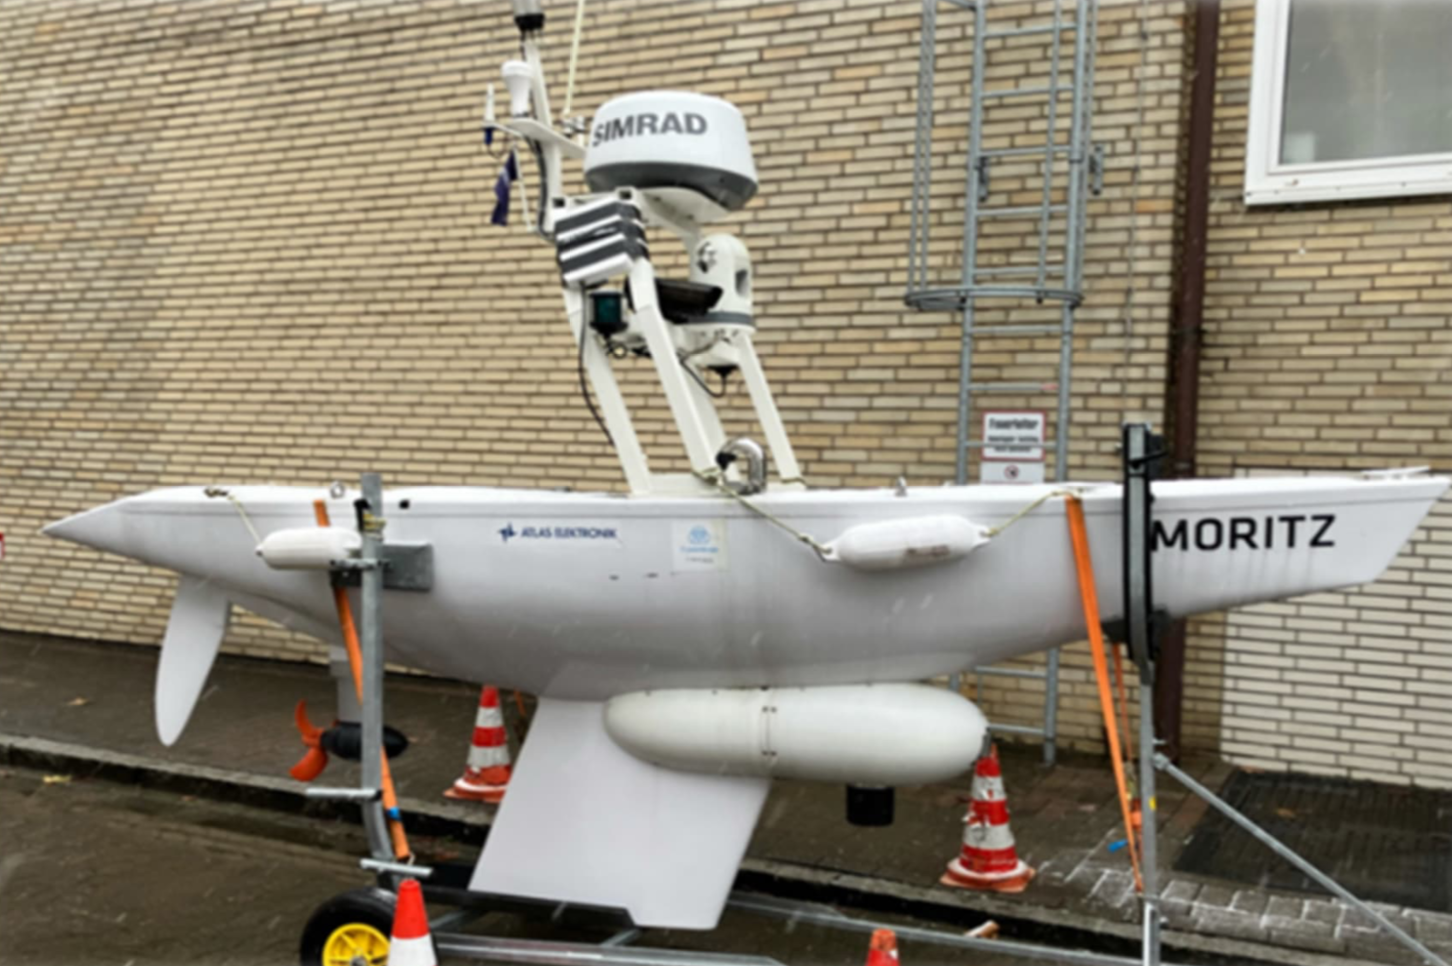
\includegraphics[scale=0.4]{image/Moritz.png} % Include image with scale
\caption{Moritz}
\label{fig:mesh1} % Label for referencing
\end{figure}
\subsection{EvoLogics Acoustic Modem}
Acoustic modems enable wireless communication underwater by using sound waves. Unlike radio frequency (RF) or optical communication, which face significant attenuation in water, acoustic communication is much more effective. This work utilizes the EvoLogics acoustic modem to facilitate data transmission between AUVs and UUVs. The modem supports full-duplex digital communication and employs advanced Sweep-Spread Carrier (S2C) technology\cite{S2C}, ensuring reliable and robust data exchange even in challenging underwater environments.

\subsection{Raspi}
The Raspi is a low-cost, credit card-sized computer designed for educational and prototyping purposes. Due to its portability, affordability, and versatility, it has become a popular choice for implementing network protocols in real-world scenarios. In this project, Raspi is a Node in the Multi-Domain Setup and the hardware platform for implementing and testing the AODV protocol. Because the protocol AODV is designed for Ad-Hoc Networks, where the device can communicate directly without relying on centralized infrastructure like a router, Raspi’s onboard wifi adapter is the most suitable due to its support for building Ad-Hoc wireless networks, enabling nodes to establish direct communication.
AODV involves route discovery, maintenance, and message Processing which requires sufficient computational power to handle these tasks. The quad-core ARMv8 processor of the Raspi provides this sufficient power. The Raspi’s multi-core processor provides a critical advantage, even when the AODV protocol is implemented in user space using Python. While Python’s Global Interpreter Lock (GIL) may limit true parallel execution within a single thread, tasks like handling multiple routing requests, processing incoming packets, and monitoring network metrics can be distributed across multiple cores using Python’s multiprocessing module or asynchronous programming techniques.

\begin{figure}[h]
\graphicspath{{/image/}} % Directory path for images
\centering
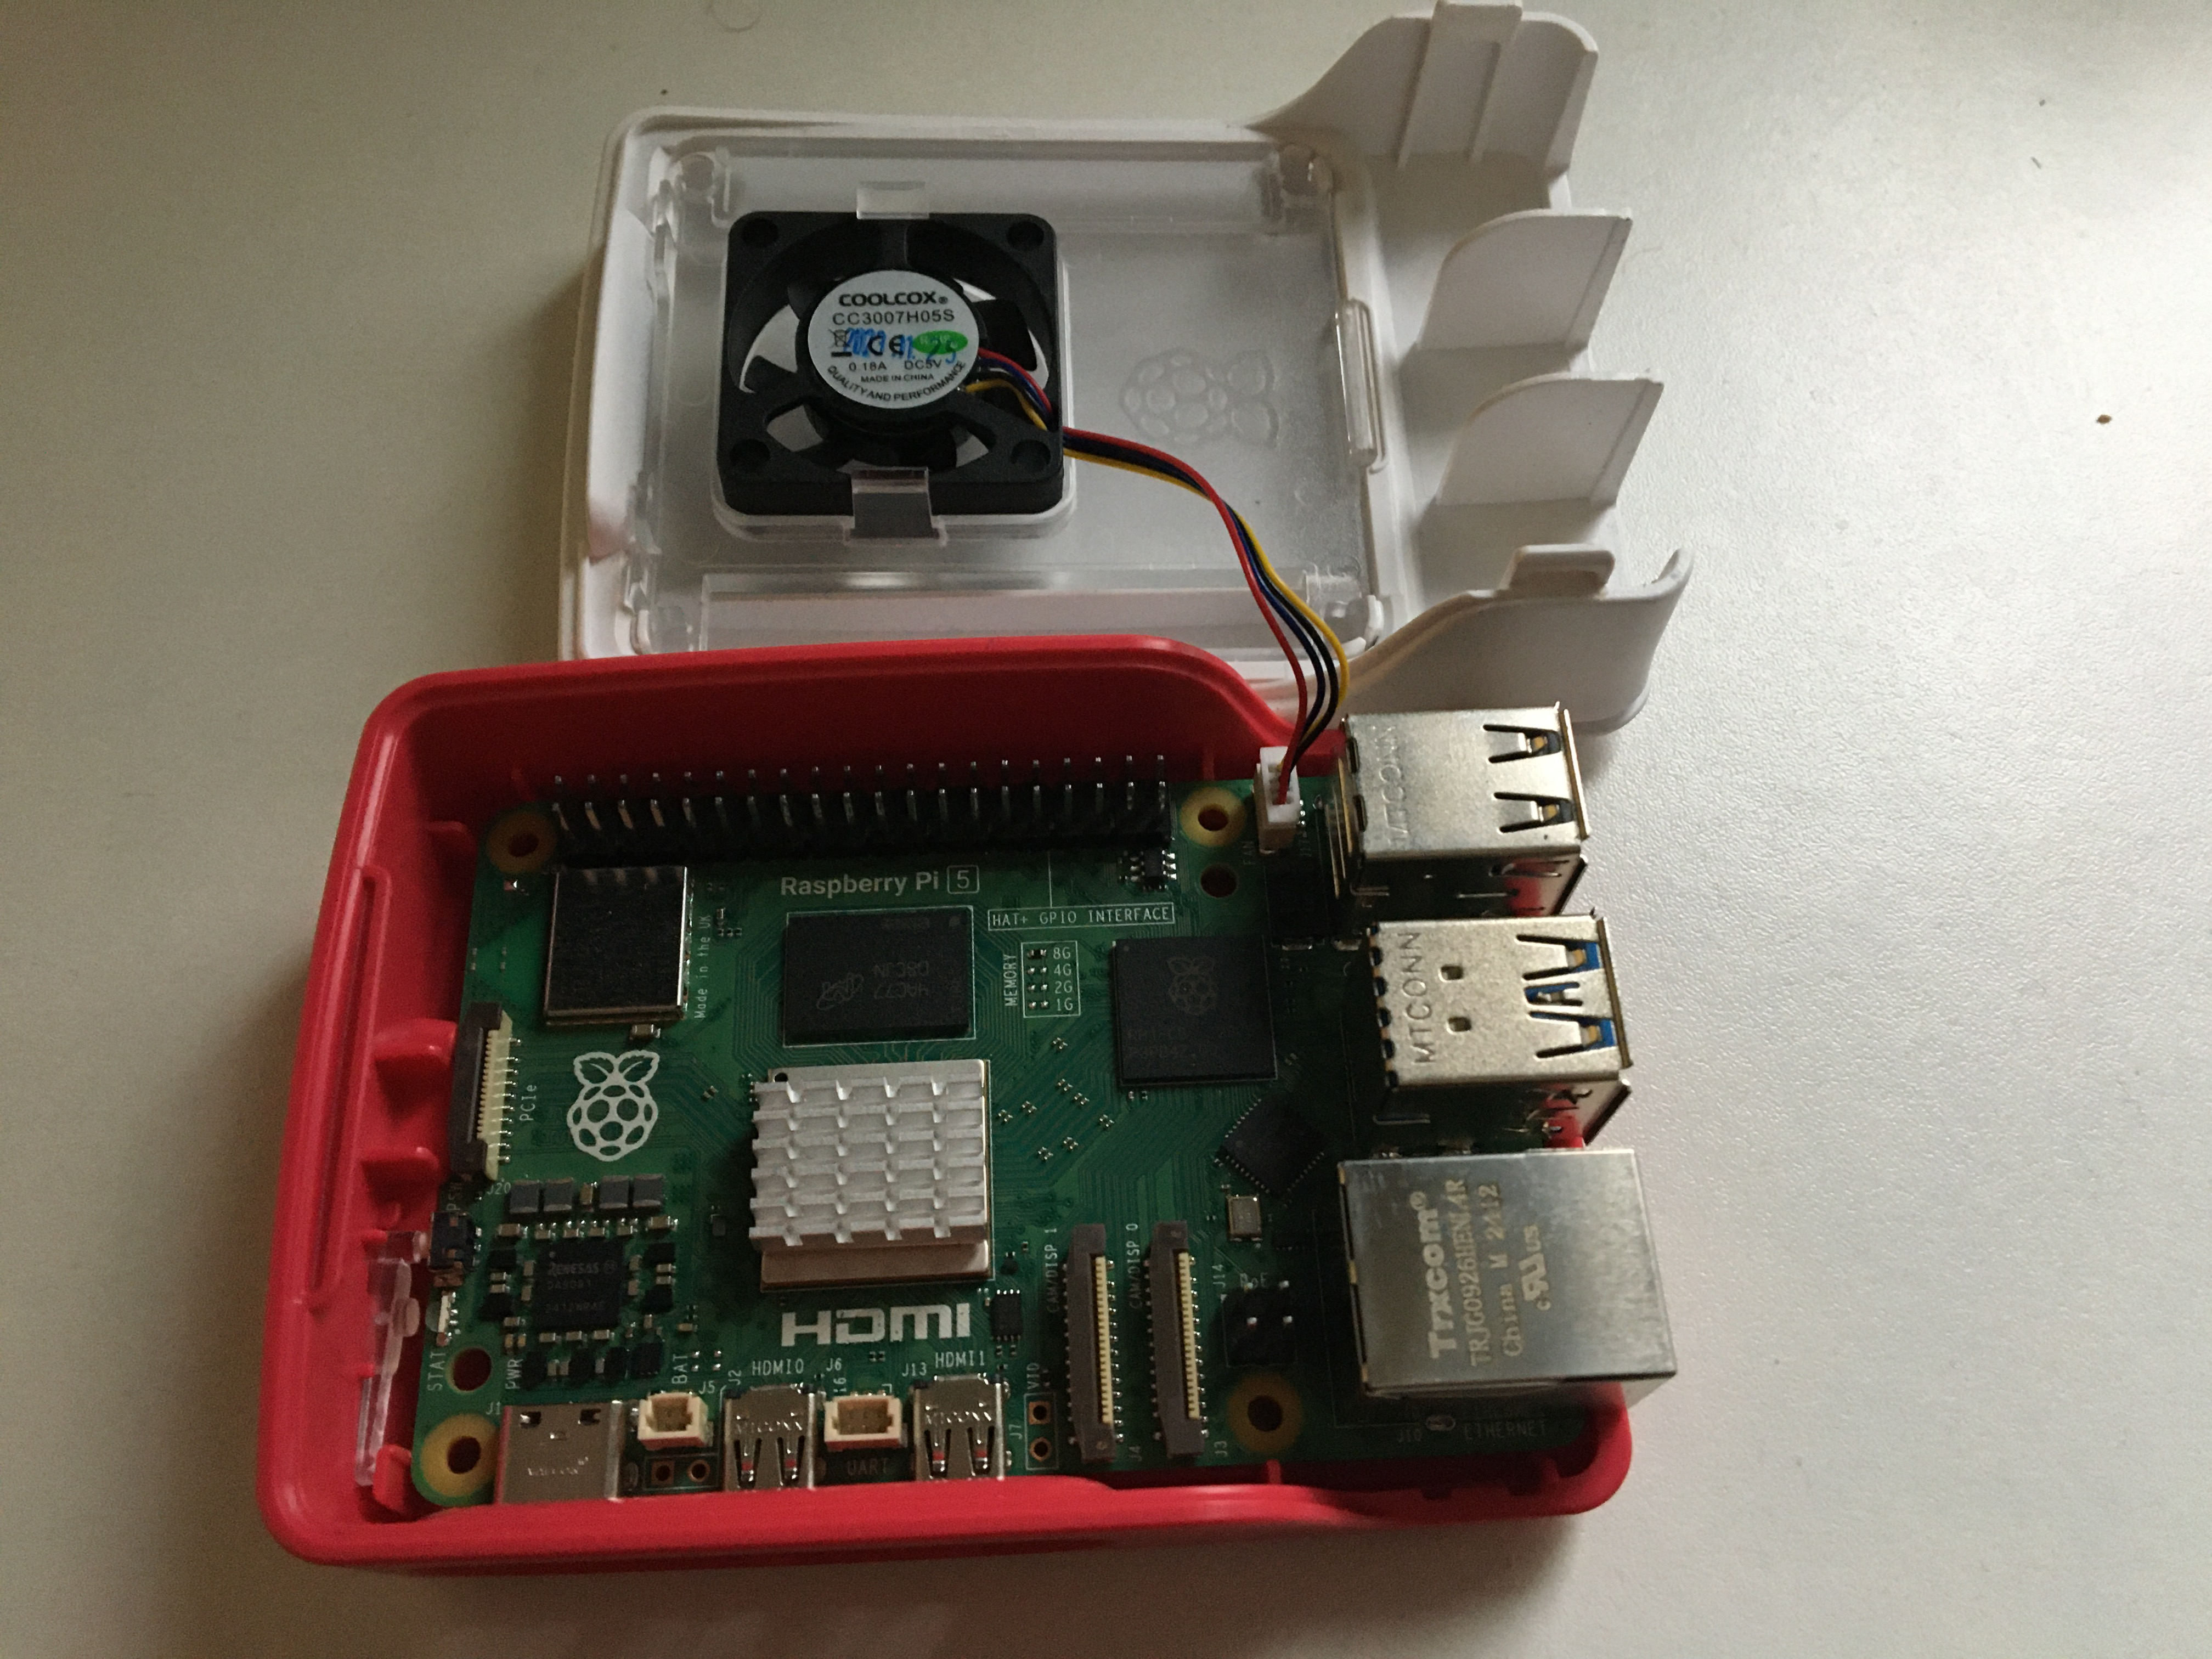
\includegraphics[scale=0.04]{image/Raspi1.JPG} % Include image with scale
\caption{Raspberry Pi 5}
\label{fig:mesh2} % Label for referencing
\end{figure}


\section{Software}
\subsection{Python}
Python's ease of use, adaptability, and vast library ecosystem make it the perfect choice for creating intricate networking protocols. Because it is a language that is easy to understand and write, it is especially well-suited for iterative development and rapid prototyping. Without needing a lot of boilerplate code, its robust standard library provides strong capabilities for managing concurrency, network connectivity, and data manipulation. Python is especially helpful for distributed systems and Internet of Things (IoT) applications because of its cross-platform nature, which guarantees that code can execute smoothly on a range of devices, including Raspi.

A constant flow of updated modules and frameworks for specialised tasks, such as networking and protocol creation, is also guaranteed by Python's community-driven development.With the help of libraries like \textbf{threading} \cite{Python} for managing concurrent processes and socket \cite{Python} for low-level network communication, developers may concentrate on the logic of protocols like AODV rather than getting bogged down by the complexities of low-level implementation. Python's adaptability also makes it possible to include debugging, testing, and monitoring tools-all of which are essential in dynamic settings like Ad-Hoc networks. Python is a strong and useful language for creating and evaluating cutting-edge networking solutions because of these characteristics.
\subsection{Raspberry Pi OS}
Rasberry Pi OS (called previously Raspbian) is a Unix-like operating system based on the Debian Linux distribution for the Raspberry Pi family of compact single-board computers.
Raspberry Pi OS comes in different versions, including Lite (minimal setup), Desktop , and Full (with additional productivity tools and software), allowing users to choose what suits their needs best \cite{Raspbian}. Raspbian version 12.8 introduces significant updates, including a shift in network management. Unlike previous versions, such as 12.7, where the default configuration relied on /etc/network/interfaces, version 12.8 emphasizes the use of dhcpcd and NetworkManager. The older /etc/network/interfaces configuration is no longer the default in this release, reflecting a modernized approach to network management.\cite{raspberrypi_interfaces_missing}
\subsection{Matlab}
MATLAB stands for MATrix LABoratory and is a high-level, interactive programming language developed by MathWorks. It is extensively used in engineering, research, and academia to solve numerical computations, data analysis, and visualization. The platform has powerful tools with built-in functions for complex mathematical solutions, such as linear algebra, signal processing, optimization, and differential equations.
MATLAB's key features include:
\begin{itemize}
    \item Numerical Computing: Matrix manipulations, data interpolation, and implementation of algorithms are enabled.
    \item Visualization Tools: Offers a powerful capability to create 2D and 3D plots, graphs, and animations for data interpretation.
    \item Toolboxes: Extends its functionality by using toolboxes for specific applications related to control systems, machine learning, image processing, and neural networks.
    \item Simulink Integration: Enables modeling, simulation, and analysis of dynamic systems using block diagrams.
\end{itemize}
MATLAB is also widely used both in academic and industrial fields due to its friendly user interface, good documentation, and large number of users. Its versatility and computation power make it an important tool to solve a wide range of engineering and scientific problems.\cite{matlab}



\chapter{State of Art }
\label{sec:fundamentals}
Concerning different fields- water or out-of-water-specific cutting-edge protocol evolution, wireless communication plays the most important role in establishing dynamic, infrastructure-less networks. Its evolution has taken new dimensions by developing innovative protocols for diverse applications, extending from mobile ad hoc networks-on-ground Mobile Ad Hoc Networks  (MANETs) to Underwater Ad Hoc Networks (UANETs). The state of the art in this domain is a reflection of increased research efforts toward improving efficiency, adaptability, and performance in communications. This chapter summarizes major strides taken both in above-water and underwater communication protocols as a basis for deep delving into their strengths, methodologies, and applications in the sections to come.
\section{MANET}
MANETs are those kinds of wireless networks that work without fixed infrastructure and centralized control; instead, they depend on nodes dynamically creating links among them to communicate. Such networks come in handy when traditional networking infrastructure is impossible to handle due to geographical constraints like a remote area, a disaster area, or even war fronts. The lack of a fixed infrastructure grants MANETs the capability of rapid deployment and adaptation to various environments, making them quite versatile for many temporary or mobile connectivity needs. Their decentralized and dynamic nature presents unique technical challenges, however, which call for innovation to ensure reliable communication with efficient network management.\cite{RFC2501}
\subsection{Features}
\begin{itemize}
    \item Decentralization: Each node in the network serves as both a host for data transmission and reception and a router for data forwarding, allowing MANET to function without centralised control.
    \item Dynamic Topology: MANETs need strong and adaptable routing techniques because node mobility causes the network topology to change constantly.
    \item Multi-hop Communication: Nodes may need to rely on intermediary nodes to relay data because they are not in direct communication range.
    \item Limited Resources: Typical limitations of MANET devices include low computing power, bandwidth, and battery life.
    \item Scalability: The network needs to manage different node densities and sizes well.
\end{itemize}

\subsection{Challenges in MANETs}
\begin{itemize}
    \item Routing: Routing protocols must be dynamic and effective due to frequent topology changes and the lack of fixed infrastructure.
    \item Security: Because MANETs are decentralized, they are susceptible to denial-of-service, impersonation, and eavesdropping assaults.
    \item Energy Efficiency: Because nodes frequently run on batteries, protocols and algorithms must be designed with energy efficiency in mind.
    \item Scalability and Performance: maintaining steady performance as the network's size and complexity increase.
    \item Interference and Reliability: Unreliable connectivity, interference, and signal deterioration can all affect wireless communication.
\end{itemize}
\subsection{Protocols in MANETs}
Specialized routing protocols provide reliable data transmission and efficient path discovery and maintenance in highly dynamic environments of the MANETs. MANET has protocols specifically designed for dynamic topologies like MANET routing protocols further classified into three core types: reactive, proactive, and hybrid.Within these categories, each protocol has defined its way of ensuring adaptability and robustness in the face of changing topologies.

Some of the most important and well-known routing protocols in MANETs include:

\begin{itemize}
    \item Ad-hoc On-demand Distance Vector (AODV) \cite{rfc3561}
    \item Dynamic Source Routing (DSR) \cite{rfc4728}
    \item Optimized Link State Routing (OLSR) \cite{rfc3626}
\end{itemize}




\section{UANET}
UANETs \cite{8976642} constitute a special class of MANET, which is developed especially to work in underwater environments. These are collections of mobile or fixed nodes (mainly underwater vehicles, buoys, and sensor nodes), that cooperate in a fully decentralized and infrastructure-less way to achieve efficient communication and data exchange.
\subsection{Features}
\begin{itemize}
    \item Acoustic Communication Medium: UANETs use acoustic waves for data transmission, which is better for long-range communication underwater compared to electromagnetic waves.
    \item 3D Topology Flexibility: With a 3D space to work in, UANETs have more freedom with their deployments and data gathering across the full scale of depths and areas of consideration.
    \item Autonomous Self-organization: Nodes in UANETs can autonomously establish and maintain communication without requiring centralized infrastructure, making them highly adaptable in dynamic underwater environments.
    \item Scalability for Diverse Applications: UANETs can range from small, localized networks for scientific exploration to large, distributed systems for military or commercial operations.
    \item Collaborative Sensing and Communication: Nodes in UANETs often collaborate to collect, relay, and process data, enabling applications such as environmental monitoring, resource exploration, and disaster management.
\end{itemize}


\subsection{Challenges in UANETs}
Critical challenges faced by UANETs make their design and operation considerably different from the terrestrial networks. First, these networks face high latency and low bandwidth because acoustic communication naturally supports slower data transmission speeds and lower bandwidth. Secondly, energy-related issues are an important problem since most of the nodes in these networks have a battery supply, and recharging or replacing them underwater is rather complicated, which requires energy-efficient solutions. The environmental factors include water currents, temperature, salinity, and pressure, along with signal attenuation and noise, which create a highly unstable communication environment. Besides, sparse node deployment is common in UANETs due to the vast underwater spaces, complicating the maintenance of connectivity and assurance of reliable data delivery. The absence of GPS signals underwater results in localization and synchronization problems, making precise node location and clock synchronization difficult. Moreover, the complicated routing in 3D topologies introduces further challenges since, in three-dimensional spaces, protocols for routing have to consider depth and distance with possible node mobility. Lastly, error-prone communication as a result of interference, scattering, and multipath effects of acoustic signals leads to higher error rates and increased packet loss. These all impose the requirement for specialized solutions that can assure effectiveness in underwater communications.

\subsection{Protocols in UANETs}
\subsubsection{Underwater Ad Hoc On-demand Distance Vector Routing(UWAODV)}
UWAODV is an underwater ad hoc on-demand distance vector routing developed to cope with the limitations of the underwater acoustic environment. Contrary to the terrestrial networks, acoustic waves have a much slower propagation speed in water compared to the speed of light in the air, around 1500 m/s, and are prone to multipath fading, Doppler shifts, and limited frequency bandwidth. These factors bring high latency, low bit rates, and high error rates that require changes in conventional protocols. UWAODV introduces two major enhancements to the issues described above. Firstly, the mechanism of flooding with retransmission (See Figure 3.1)is introduced for Route Request packets to ensure their reliable delivery by compensating for errors and losses due to the harsh underwater channel. This reduces congestion and delays, hence making network performance more stable. The proposed remaining routing mechanism of reservation-based residual routing mechanism works in managing the routes efficiently, extending the timer expiry time and therefore avoiding rediscovery processes when not necessary; it conserves important resources for other network uses. UWAODV outperforms standard AODV, with regard to simulations carried out within the OMNET++ environment by improving the packet delivery ratio from 75.4\% to 81.9\%, decreasing the time of route setup by about 29.7\%, and an overall end-to-end delay by about 20\%. \cite{7879681}

\begin{figure}[h]
\graphicspath{{/image/}} % Directory path for images
\centering
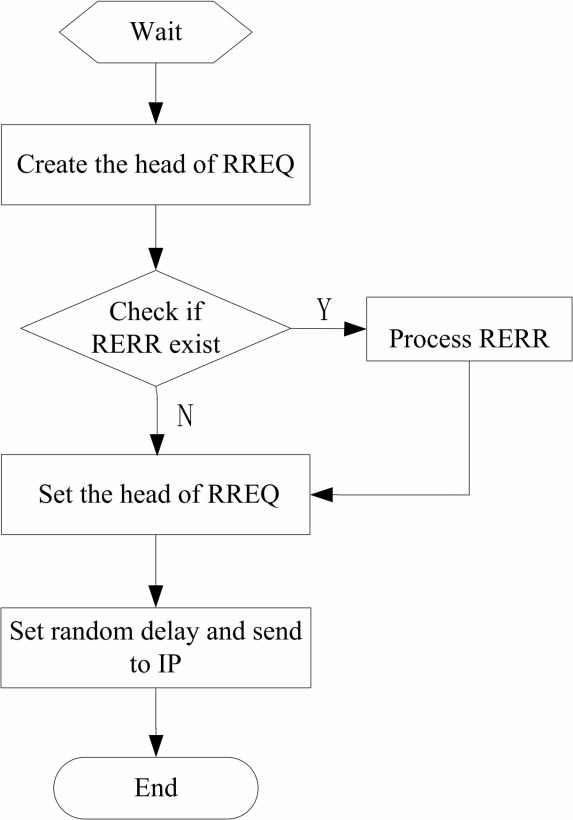
\includegraphics[scale=0.4]{image/Doubling flooding.png} % Include image with scale
\caption{Doubling flooding \cite{7879681}}
\label{fig:mesh2} % Label for referencing
\end{figure}
\clearpage
\subsubsection{AODV- for sparse underwater acoustic routing protocol
(AODV- SUARP)}
AODV-SUARP is one underwater-specific routing protocol. AODV-SUARP has increased communication in 3D underwater sensor networks by deploying sensors in layered topology that employs both acoustic and radio modems. The working of AODV-SUARP encompasses two major phases: route finding phase and data forwarding phase. During the route finding phase, source nodes broadcast a Route Requisition Message RRQ with the intent of discovering the route. Upon receiving the RRQ, the destination node executes a route stability function by assessing possible paths regarding energy level and hop count and labels these routes as "strongest", "stronger", and "strong" based on the energy of sensor nodes within that route. This function enables the destination node to choose the most energy-efficient and reliable paths for data transmission, ensuring that only the most capable paths are used to prolong the operational life of the network. AODV-SUARP is particularly suitable for sparse underwater environments where energy efficiency and reliability are of high importance owing to the difficult conditions of underwater communication.\cite{9907973}
\subsubsection{Vector-Based Forwarding(VBF)}
VBF is a geographic routing protocol designed for UANETs to cope with such issues as sparse node deployment, dynamic topology, and energy constraints. VBF works by defining a "routing vector" between the source and destination, and only nodes within a predefined "forwarding zone" around this vector participate in packet forwarding. This approach minimizes unnecessary flooding, reduces redundant transmissions, and saves the limited energy resources of underwater nodes. The protocol also effectively mitigates packet collisions by restricting forwarding to relevant nodes, thus efficiently utilizing the constrained underwater bandwidth. VBF is inherently adaptive to node mobility due to underwater currents, as forwarding decisions are made based on real-time node positions in a dynamic manner. All of these characteristics make VBF a robust and energy-efficient solution for the unique challenges imposed by UANET communication.\cite{10.1007/11753810_111}
\clearpage
\begin{figure}[h]
\graphicspath{{/image/}} % Directory path for images
\centering
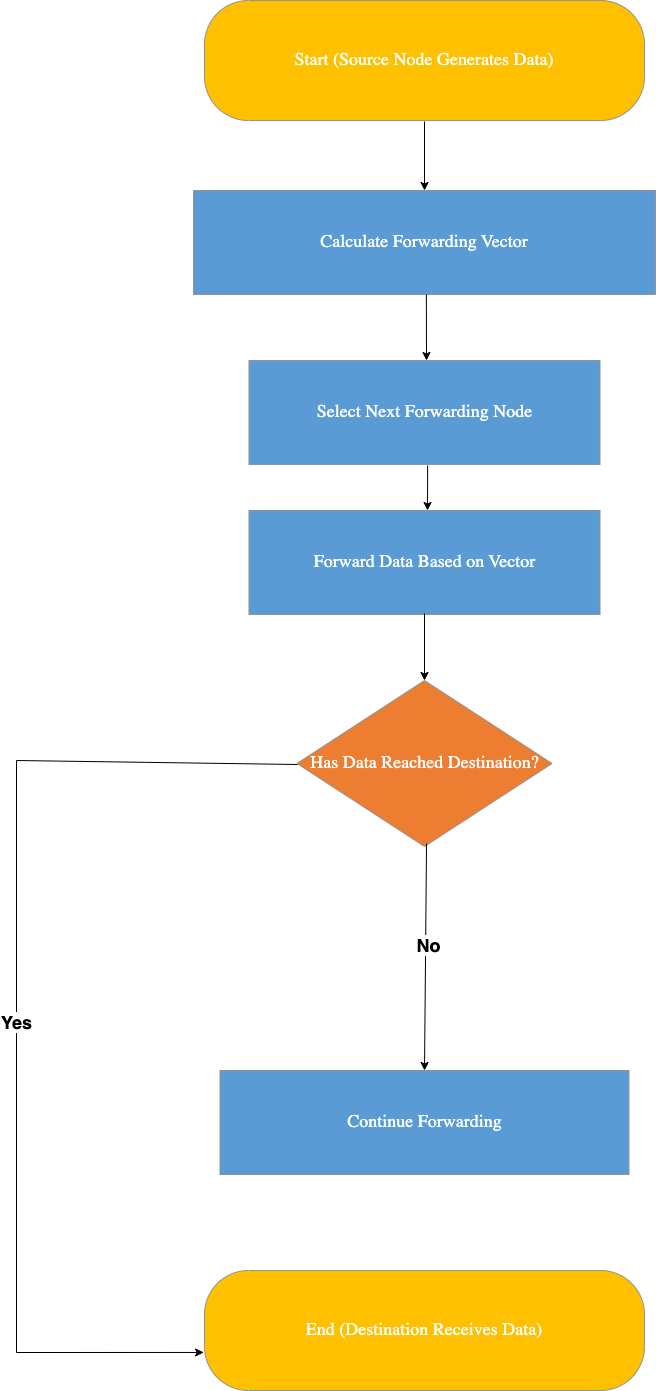
\includegraphics[scale=0.4]{image/Untitled Diagram.drawio.png} % Include image with scale
\caption{Vector-Based Forwarding\cite{10.1007/11753810_111}}
\label{fig:mesh2} % Label for referencing
\end{figure}
\clearpage
\subsubsection{Depth-Based Routing(DBR)}
DBR is a depth-exploitation routing protocol, specially designed for underwater sensor networks, which uses the vertical dimension to increase data transmission efficiency. Within DBR, the organization of sensor nodes is based on their depth level. At the same time, the data routing decision depends on selecting an optimum depth node to forward data toward its destination, usually the sink node. The depth-based protocol minimizes energy consumption due to the reduced need for network-wide continuous communication. It thus ensures reliable data transmission in the challenging underwater environment where traditional flat routing protocols fail for various reasons, including high latency, limited bandwidth, and energy constraints. In this way, DBR helps prolong the lifetime of sensor nodes, avoids excessive communication overhead, and optimally routes towards better energy efficiency and reliability in data delivery. It thus targets the localized depth-based routing principle that avoids unnecessary energy consumption by ensuring effective data flow. Its application is ideally suitable in underwater environments for applications that include long-term monitoring tasks regarding environmental sensing, habitat monitoring, and autonomous underwater vehicle communication. In underwater communications, the environment is normally so harsh; hence, energy efficiency and reliability become vital.\cite{10.1007/978-3-540-79549-0_7}

\begin{figure}[h]
\graphicspath{{/image/}} % Directory path for images
\centering
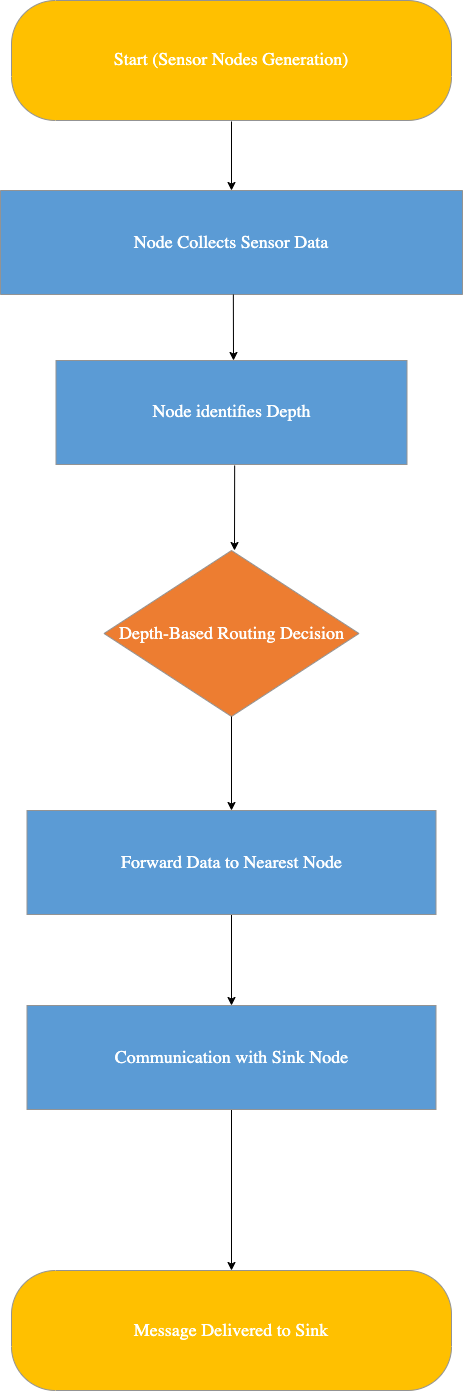
\includegraphics[scale=0.4]{image/Untitled Diagram.drawio (1).png} % Include image with scale
\caption{Depth-Based Routing\cite{10.1007/978-3-540-79549-0_7}}
\label{fig:mesh2} % Label for referencing
\end{figure}
\clearpage
\section{Simulation's Frameworks of MANET}
Simulation frameworks are vital for the design, testing, and evaluation of MANETs. These tools allow researchers to create a controlled and reproducible environment to study network behavior across various scenarios, eliminating the need for expensive physical setups. They are crucial for assessing the performance of routing protocols, mobility models, and scalability in the dynamic and unpredictable environments typical of MANETs.

Each simulation framework comes with distinct features that cater to specific research requirements. They differ in scalability, user-friendliness, supported protocols, and the realism of their modeling capabilities. Notable simulation tools include OMNeT++, NS-2,  NS-3,and Matlab, all of which have gained significant traction in both academic and industrial circles for MANET research.
\begin{itemize}
    \item \textbf{OMNeT++:} This is a modular, extensible, and component-based C++ simulation library that is especially well-suited for modeling complex networks and can be easily integrated with external libraries. \cite{omnetpp}
    \item \textbf{NS-2 and NS-3:} NS-2 is one of the earliest and most influential simulation tools, offering support for a diverse array of network protocols and models. However, it has largely been surpassed by NS-3, its newer and improved version. NS-3 was developed to address the shortcomings of NS-2, providing better realism, scalability, and enhanced capabilities, making it the preferred choice for current MANET research.\cite{10.1145/1878537.1878651}
    \item \textbf{Matlab:} MATLAB is a high-level programming language and computing environment that is widely used for prototyping, developing algorithms, and running simulations. Although it wasn't specifically created for MANETs, MATLAB offers the flexibility needed to implement and simulate various wireless network protocols, mobility models, and performance metrics. Its robust visualization features and comprehensive toolbox support make it an excellent choice for validating and analyzing network behaviors.\cite{mathworks_wireless_network}

    
\end{itemize}
Each of these frameworks has distinct advantages suited to various elements of MANET simulations. Choosing the right tool hinges on particular research needs, including the desired level of detail, scalability, and ease of implementation. In the upcoming subsections, we will explore the use of MATLAB, OMNeT++, and NS-2/NS-3 as simulation frameworks for MANETs, emphasizing their features and significance in simulating scenarios specific to MANETs, such as dynamic topology, routing protocols, and node mobility.
\subsection{OMNeT++}
The application of OMNeT++ for the modelling of MANETs based on its modularity, extensible libraries and event-driven architecture is described. Its modular architecture allows for the decoupled implementation of components (e.g., routing, MAC, and the physical layer) and development without interference and testing. The INET Framework adds to OMNeT++ the needed protocols (TCP/IP and UDP)\cite{idserda2004tcp} for a MANET, and also includes various MAC layer specifications (IEEE 802.11), which are the fundamental building block for a MANET city. On the other hand, OMNeT++ is a session of event-oriented systems and the network behaviors, e.g., packet, nodes and device behaviors, are simulated. These capabilities lay the foundation for OMNeT++ as a powerful modeling and simulation platform for MANET dynamics under a wide range of circumstances.

Two of the most popular simulated Ad Ad-Hoc protocols in OMNeT+ are AODV \cite{parmar2014performance} and DSR\cite{bhatia2016comparative}. These protocols are carried out in the form of standalone modules in OMNeT+, and subsequently combined as submodules of the MANET Manager. The MANET Manager serves as a central module that oversees routing operations and facilitates interactions between the IP layer and ad hoc routing protocols(see figure 3.1). It is responsible for triggering routing processes (e.g., route discovery), modifying the IP tables following route discovery, and completing the initialization of the routing table. In OMNeT+ events, such as packet transmission and protocol communication, are modeled as messages so that each module could generate, process, or even forward them according to its purpose. This modular approach allows for detailed simulation of network behaviors, including routing and node interactions in MANET scenarios.
\begin{figure}[h]
\graphicspath{{/image/}} % Directory path for images
\centering
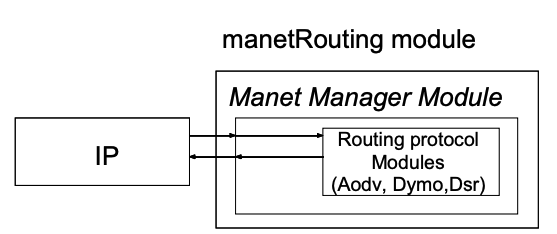
\includegraphics[scale=0.6]{image/Manet routing.png} % Include image with scale
\caption{MANET Module\cite{ariza2008implementation}}
\label{fig:mesh3} % Label for referencing
\end{figure}
\subsection{NS-2}
The Network Simulator 2 (NS-2) is the most widely used simulation environment for MANETs, offering the most robust support for proactive routing protocols like DSDV and reactive protocols such as AODV and DSR\cite{refId0}. NS-2 is based on a dual-language architecture: C++ and Object-oriented Tool Command Language (OTcl). The C++ provides the backend, which defines the fundamental mechanisms for simulation objects, while OTcl acts like a frontend that provides a user with the capability to build simulations through assembling, configuring, and scheduling discrete events. This division of labor allows flexibility and efficiency in simulating complex network behaviors.(see figure 3.2)

MANET protocols implementation in NS-2 will represent accurate modeling of node behavior, topology dynamics, protocol functionality, and communication traffic(see figure 3.3). The nodes within the network are mobile by nature, having their movements and communication ranges explicitly defined. Dynamic topologies are produced with the help of third-party utilities like "setdest" from CMU, which configures node mobility and positions within the simulation environment. NS-2 supports detailed protocol simulations for proactive protocols, such as DSDV, and reactive protocols, such as AODV and DSR, through which realistic modeling of critical processes like route discovery and maintenance can be done. The simulation of traffic and communication is made possible with the use of tools such as "cbrgen.tcl," which models traffic patterns, including TCP and CBR connections between nodes. These simulations capture key performance metrics such as packet delivery ratios, delays, and throughput that provide valuable insight into the behavior and efficiency of MANET protocols for different scenarios.
\begin{figure}[h]
\graphicspath{{/image/}} % Directory path for images
\centering
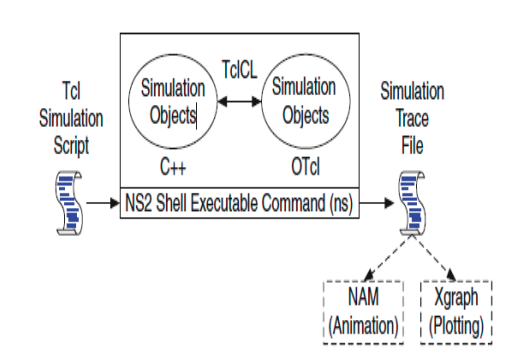
\includegraphics[scale=0.4]{image/Architectur_of_NS.png} % Include image with scale
\caption{Basic architecture of NS\cite{al2018performance}}
\label{fig:mesh4} % Label for referencing
\end{figure}
\clearpage
\begin{figure}[h]
\graphicspath{{/image/}} % Directory path for images
\centering
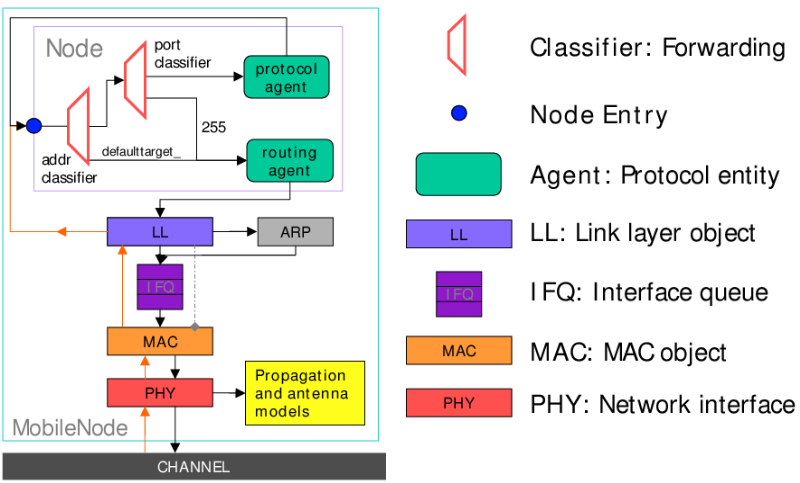
\includegraphics[scale=0.4]{image/Node Modell Ns-2.png} % Include image with scale
\caption{Wireless node model in Ns2 \cite{al2018performance}}
\label{fig:mesh5} % Label for referencing
\end{figure}



\subsection{NS-3}
NS-3 provides tools and modules specifically tailored for simulating MANETs, enabling researchers to analyze protocols like AODV, OLSR, and DSR under various conditions. The platform’s ability to incorporate mobility models and diverse traffic scenarios allows for evaluating the performance of MANET protocols in terms of metrics like delay, throughput, and packet delivery ratio.

The NS-3 simulator is a novel one. It isn't NS-2's expansion. It is not compatible with the NS-2 APIs. All of it is written in C++, while Python bindings are optional. Because of this, simulation programs can be developed in Python or C++. Since the oTcl scripts are no longer required to manage the simulation, the issues brought about by the mix of C++ and oTcl in NS-2 are resolved. NS-3 is therefore a far more user-friendly and easily expandable platform. 

NS-3 has modern recreation highlights, which incorporate
broad parameterization framework and configurable implanted
following framework, with standard yields to content logs or PCAP
(tcpdump). It is exceptionally question arranged for fast coding and
expansion. It has an programmed memory administration capability
as well as an productive question aggregation/query for unused
behaviors and states, like including portability models to hubs.
Additionally, NS-3 has modern capabilities, such as taking care of
numerous interfacing on hubs accurately, productive utilize of IP
tending to and more arrangement with Web conventions and
plans and more nitty gritty 802.11 models. NS-3 coordinating
the structural concepts and code from GTNetS\cite{1261483} , which
could be a test system with great adaptability characteristics. The
Reenactment Arrange Design looks a bit like IP design
stack. The hubs in NS-3 may or may not have portability. The
hubs have "arrange devices", which exchange bundles over
channel and joins Layer 1 (Physical Layer) and Layer 2
(Information Connect layer). The organize gadgets acts as an interface
with Layer 3 (Arrange Layer: IP, ARP). The Layer 3 bolsters
the Layer 4 (Transport Layer: UDP, TCP), which is utilized by the
Layer 5 (Application Layer) objects.(see figure 3.4)

\begin{figure}[h]
\graphicspath{{/image/}} % Directory path for images
\centering
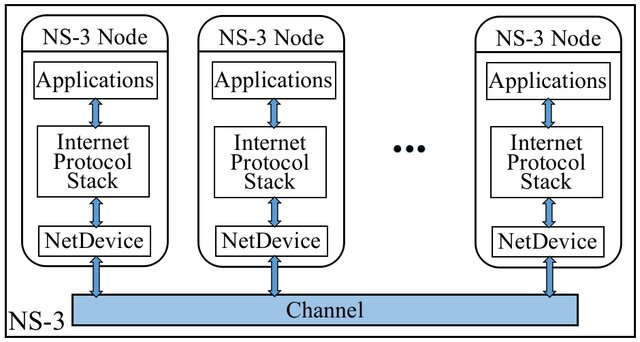
\includegraphics[scale=0.4]{image/Data-flow-model-in-NS-3-Simulation-at-a-High-level_W640.jpeg} % Include image with scale
\caption{NS-3 Nodes \cite{article}}
\label{fig:mesh6} % Label for referencing
\end{figure}

\subsection{Matlab}
MATLAB is one of the most impressive tools to simulate MANET applications, offering robust computational capacities, visualization facilities, and a well-equipped programming environment. Using this application, one can effectively simulate the MANET, because it uses very advanced models to define mathematical and algorithmic processes and it has powerful visualization instruments that are used to visualize the dynamic evolution of a network topology.

Simple MANET is a project for those who have accessed MATLAB and it targets mainly the researchers and students. The Simple MANET project simplifies the operation of simulating MANETs without going through numerous setups and has provided an easy-to-use, out-of-the-box environment that's very powerful. With the novel graphics power of MATLAB, it visualizes the dynamic topology of MANETs and hence appears to prove some real-life phenomena like node mobility and link failures.

Simple MANET allows users to create and change the AODV  or DSR  MANET protocols by writing their own functions or classes. Also, MAC protocols such as ALOHA, CSMA, and TDMA will be studied using a specific class called LinkModel. This modular aspect allows for easy experimentation and extension of various network protocols.

Simple MANET is an expression of the flexibility of MATLAB, since it would support many of the simulation scenarios by parameterized configuration. Users would be able to specify simulation parameters such as node numbers, topology areas, and simulation time, thus enabling a comprehensive consideration of different possible network behaviors and arrangements.

In fact, Simple MANET clearly demonstrates one of the ways that MATLAB can rapidly excite creativity and enables innovative designs in the modeling process to create visualization interfaces to MANET simulations.\cite{iuriivoitenko2021simplemanet}
\section{MANET Implementation on Raspberry Pi}
Most of the research on MANET implementation with Raspberry Pi devices focuses on the evaluation and comparison of various routing protocols, such as AODV, Better Approach to Mobile Ad hoc Networking (B.A.T.M.A.N.) and OLSR. Raspberry Pi devices provide an easy platform on which these protocols can be tested in real-life scenarios to gain insight into their performance under dynamic network conditions. AODV is best suited for minimizing overhead with its on-demand route discovery, while OLSR applies proactive routing with periodic updates to maintain better route stability. B.A.T.M.A.N., on the other hand, proposes a decentralized routing approach that relies on the quality of the local links to enhance scalability and adaptability in high-mobility or dense MANET scenarios. These protocols are implemented on Raspberry Pi testbeds for detailed comparisons with respect to latency, packet delivery, and energy efficiency to provide insights into MANET applications.
\subsection{AODV Implementation on Raspberry Pi}
The implementation of AODV protocol on Raspberry Pi has advanced significantly, with AODV-UU serving as a widely adopted framework due to its stability and adaptability. Originally developed for older Linux kernels (e.g., 2.6 and 3.8), AODV-UU faced compatibility challenges with newer kernels, such as Linux 4.15, commonly used on Raspberry Pi platforms. These challenges were addressed by updating the implementation to align with modern kernel architectures.

Key improvements included replacing deprecated kernel functions and removing dependencies on outdated modules, such as libipq and kaodv. These updates not only ensured compatibility with newer kernels but also enhanced the modularity and security of the implementation. The adoption of modern packet management techniques within Netfilter, a crucial Linux subsystem for packet filtering and routing, played a central role in this transition, allowing efficient message handling for route discovery and maintenance.

Leveraging these updates, Raspberry Pi nodes configured in ad hoc wireless mode provide a cost-effective and portable testbed for MANET experimentation. Validation tests demonstrated the updated implementation's ability to establish routes dynamically, maintain accurate routing tables, and enable reliable packet transmissions under various scenarios. These advancements solidify AODV-UU’s position as a practical solution for reactive routing protocol research, offering a foundation for performance evaluation in areas such as packet delivery ratio, latency, and energy efficiency.\cite{9059478}

\begin{figure}[h]
\graphicspath{{/image/}} % Directory path for images
\centering
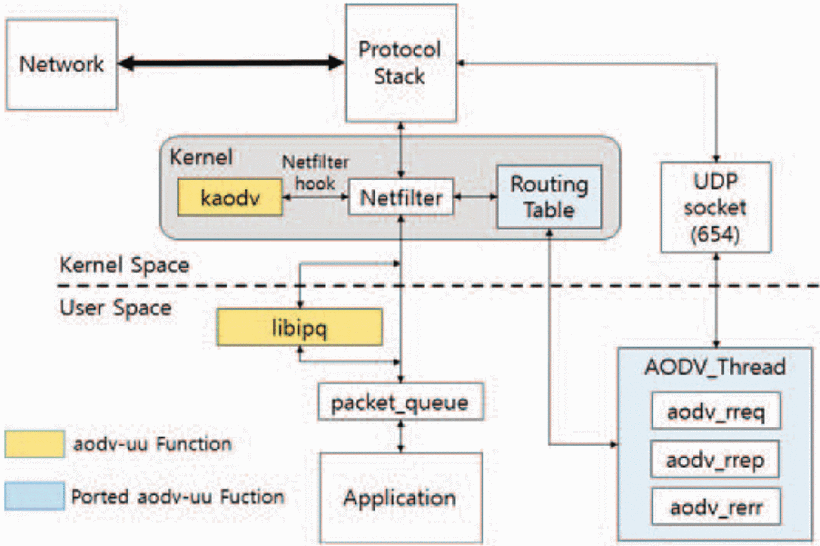
\includegraphics[scale=0.4]{image/AODV-UU.png} % Include image with scale
\caption{AODV-UU Architecture \cite{9059478}}
\label{fig:mesh6} % Label for referencing
\end{figure}




\subsection{B.A.T.M.A.N Implementaion on Raspberry Pi}
The implementation of B.A.T.M.A.N. on Raspberry Pi has been extensively studied as a practical approach to establishing efficient and scalable MANETs. B.A.T.M.A.N. operates as a proactive Layer 2 mesh routing protocol, simplifying route discovery by handling Ethernet frames directly, which eliminates the complexity of higher-layer routing. Its ability to optimize end-to-end throughput using metrics like link quality and bottleneck throughput makes it particularly suited for resource-constrained environments. On Raspberry Pi, the implementation leverages the batman-adv kernel module, enabling mesh routing through the integration of ad hoc wireless interfaces. By configuring the Raspberry Pi's Wi-Fi module in ad hoc mode, nodes can communicate directly without relying on centralized infrastructure. Research has shown that deploying B.A.T.M.A.N. on Raspberry Pi provides a robust platform for evaluating mesh networking performance under varying network conditions, including static and mobile topologies. This combination has been utilized for diverse applications, such as IoT networks, rural communication systems, and disaster recovery scenarios. The modularity and affordability of Raspberry Pi make it an ideal choice for studying B.A.T.M.A.N.’s real-world behavior, allowing researchers to explore scalability, throughput optimization, and dynamic topology adaptation in MANET environments.\cite{10639789}
\subsection{OLSR Implementation}
Optimized Link State Routing implementation on Raspberry Pi has been a hot topic in wireless ad hoc network development, especially in content-centric scenarios. OLSR is a proactive routing protocol that refreshes the routing information periodically through the exchange of control messages, ensuring stable and efficient routes in the network. Research has utilized the Raspberry Pi platform for OLSR deployment due to its cost-effectiveness, portability, and versatility. For example, one testbed that combined the use of Raspberry Pi devices with OLSR has been implemented for wireless content-centric networking. It lets nodes act as publishers or consumers dynamically to share or request content over a MANET while always maintaining high performance of the throughput and latency in cases where network conditions are dynamic. Such studies validate the practicality of using Raspberry Pi for real-world OLSR applications in environments like disaster recovery, IoT networks, and mobile media dissemination.\cite{7424834}




\chapter{Methods}
\section{Design and Development}
The Design and Development phase becomes a very important part of the methodology during which the artifact could be innovative solutions to the identified problems- conceived, constructed, and valiantly iterated. In this thesis, the artifact is a communication framework through which underwater and surface nodes are linked using a USV as a gateway. The innate AODV routing protocol is incorporated within the framework to support dynamic route discovery and maintenance and to address issues of heterogeneous integration.

This particular point is being concentrated on building a really solid system that will cater to dynamic topologies, mobility, and the reliability of communication from underwater to surface nodes through a USV gateway in this system.
\subsection{System Overview}
This study talks about the whole system architecture for assessing the multiple-domain communication networks for land, air, and sea environments including the underwater domain. The system consists of three important components: above-water nodes(UAV), surface nodes(USV),  and underwater nodes(UUV). The underwater nodes communicate acoustically, an energy-efficient means for long-range communication in an aquatic environment. The above-water nodes will directly communicate through RF to achieve high-speed and high-bandwidth data transmission, for facilitating interaction both among UAVs and between UAVs and USVs. Moreover, the UAVs will establish an amphibious link between above-water and underwater processes by using acoustic signals for communicating with UUVs, which will ensure seamless communication between the domains. This solution fulfills the requirements of a robust and scalable communications environment for a variety of operational environments.
\begin{figure}[h]
\graphicspath{{/image/}} % Directory path for images
\centering
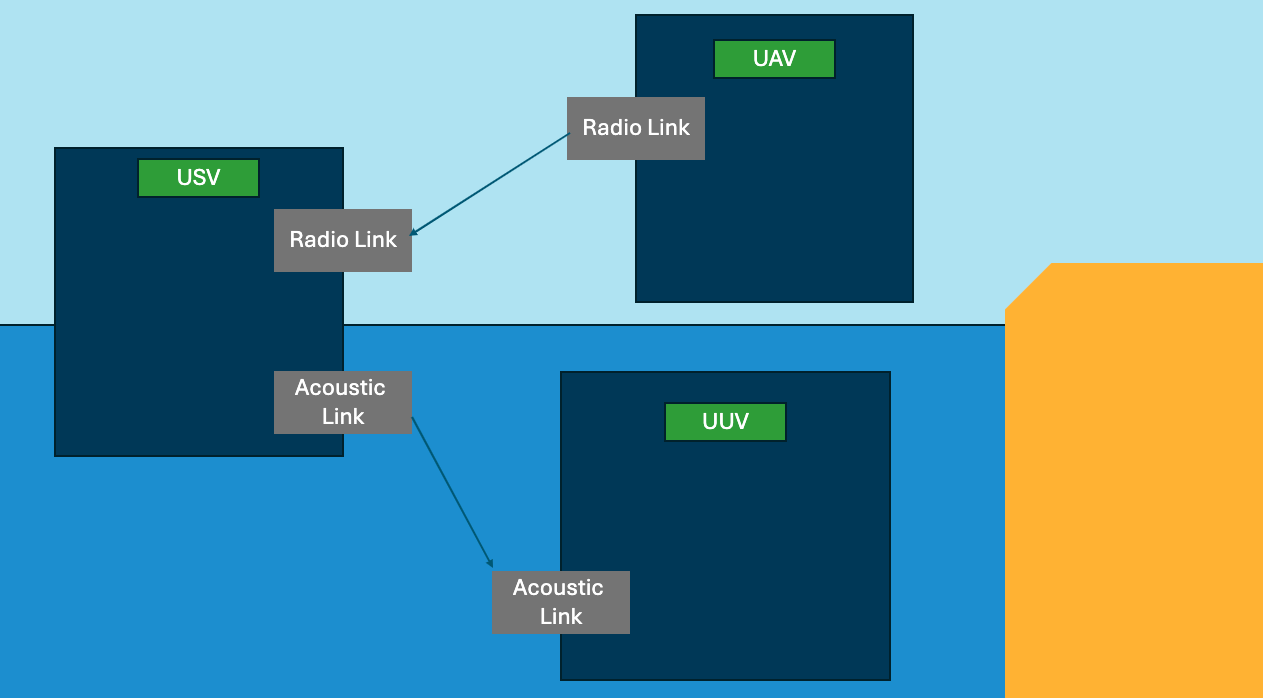
\includegraphics[scale=0.27]{image/Bildschirmfoto 2025-01-08 um 23.41.15.png} % Include image with scale
\caption{Systeme Overview}
\label{fig:mesh7} % Label for referencing
\end{figure}
\subsection{AODV Protocol}
The currently developed model in this research builds the system on a tried-and-proven AODV protocol as a building block to design the entire protocol. Further works have been accomplished on the AODV protocol to fuse the nodes residing underwater with nodes above the water level to allow communication between the parts of air and those underwater. The following sections would discuss the significant characteristics of AODV and changes made to it for successful integration over these two environments.
\subsubsection{Key Features of AODV}
One of the important features of AODV is the route discovery on demand , wich  used as the core of this design in the System Architectur.this Route discovery has two main function wich are :
\begin{itemize}
    \item \textbf{ROUTE REQUEST:}When a node communicates in the MANET network and has no known route at a given time ,it broadcast Route Request (RREQ) message(See figure 4.1).This normally normally propagates through the network until it reaches its destination .
    \item \textbf{ROUTE REPLY:} To complete the process of builduing the route between the source and the receiver ,the receiver send a unicast message called Route Reply(RREP) as a respond for the RREQ from the sender. (See figure 4.2)
\end{itemize}
These features is maintained when there is above-water communication. However, if the node is submerged below the water surface, then the challenges will be focused on due to a hostile above water environment, such as interference and overall RF signal attenuation. Hence, there should be a modification of the AODV protocol mechanisms to fit the underwater domain in our communication system.
\begin{figure}[h]
\graphicspath{{/image/}} % Directory path for images
\centering
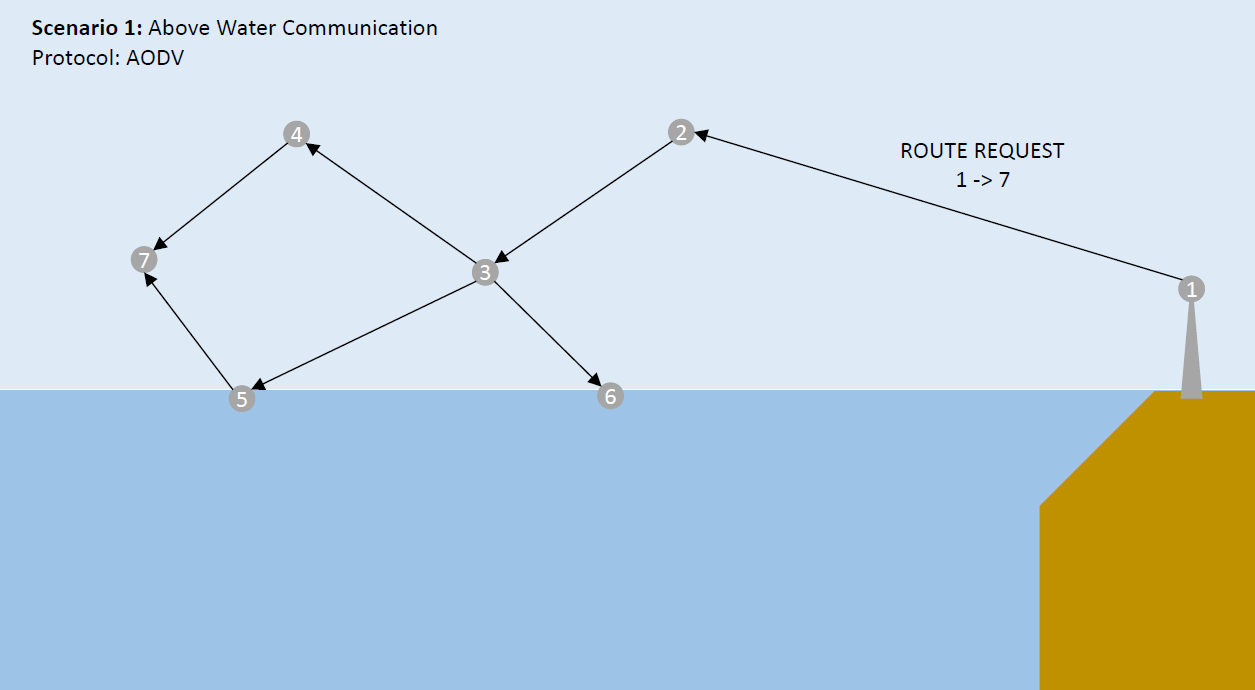
\includegraphics[scale=0.5]{image/Scenario1.png} % Include image with scale
\caption{Route Request Broadcast}
\label{fig:mesh7} % Label for referencing
\end{figure}
\begin{figure}[h]
\graphicspath{{/image/}} % Directory path for images
\centering
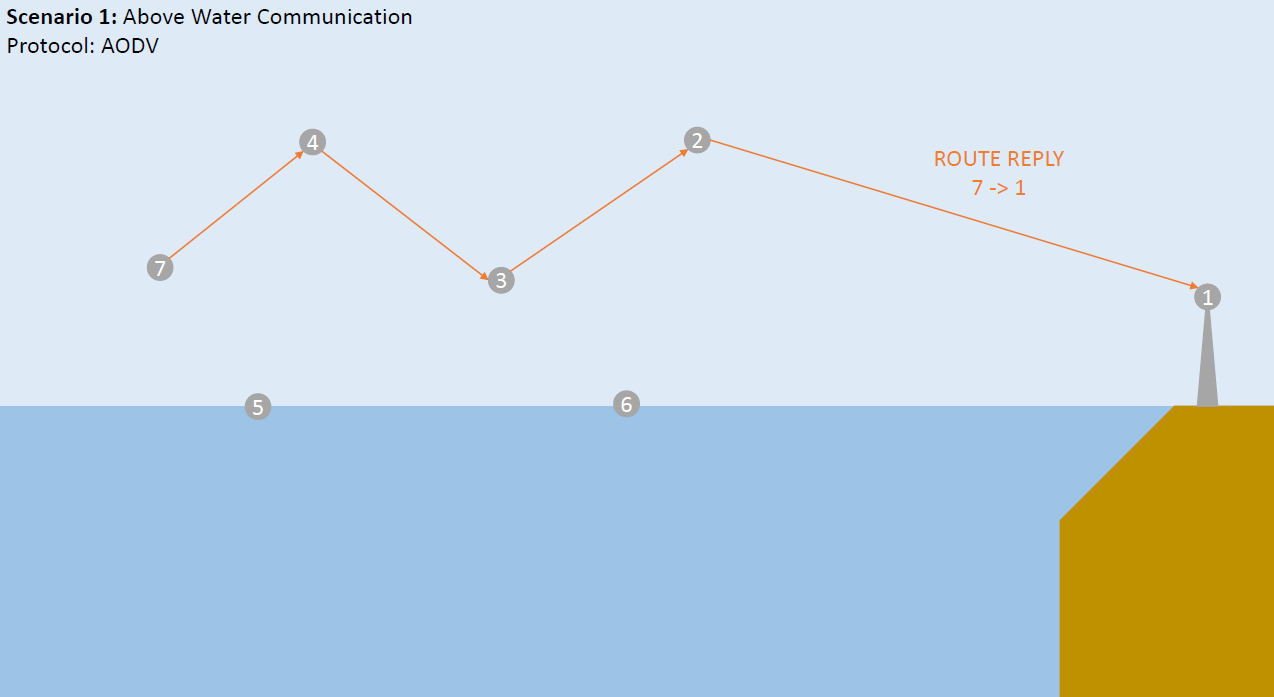
\includegraphics[scale=0.5]{image/Scenario1_2.png} % Include image with scale
\caption{Route Reply responce}
\label{fig:mesh8} % Label for referencing
\end{figure}
\clearpage

\subsubsection{Adaptations for Underwater Communication}
Communication between above-water nodes and submerged underwater nodes presents a unique challenge due to the properties of the aquatic environment. When a node above water sends a route request (RREQ), the RF signal used in traditional AODV routing rapidly attenuates as it enters seawater due to its high conductivity and permittivity. As a result, communication through RF signals becomes ineffective when the destination node is submerged.

To enable communication with underwater nodes, acoustic signals are required beneath the water. Acoustic communication, although slower than RF communication, can effectively facilitate long-range data transfer underwater. To bridge the gap between above-water and underwater nodes, a gateway device such as a buoy or USV is necessary to forward data packets. These gateways must support both RF signals for above-water communication and acoustic signals for underwater communication, enabling a seamless transition between the two modes of communication.

In this hybrid system, the gateway node functions as a critical link in the network, facilitating communication between the above-water and underwater nodes. The gateway must have dual interfaces: one to communicate with above-water nodes via RF signals and another to communicate with underwater nodes using acoustic signals.

When an above-water node attempts to establish a route to a submerged node, it first sends out a route request (RREQ) as per the AODV protocol. However, if the destination node is submerged underwater, and the RREQ does not receive a response, the protocol needs to handle this situation efficiently. The issue arises because the RREQ cannot reach the underwater node directly, and the typical RF communication fails to penetrate the water. Therefore, the system must rely on a mechanism that communicates specifically with the gateway nodes, facilitating the transition from RF-based to acoustic-based communication.

After the timeout period in which no route reply (RREP) is received, the node will broadcast a new message called the "Relay Request." This message is similar to the RREQ but is directed only to the gateway nodes. All other nodes will forward the message without responding to it. The gateway nodes, upon receiving the Relay Request, respond with a "Relay Reply" , which serves the same function as the traditional RREP but includes coordination with the gateway for optimal selection.

This mechanism ensures that the gateway nodes facilitate the transition of data from RF communication to acoustic communication, effectively bridging the gap between above-water and underwater nodes. The Relay Reply sent by the gateway contains the necessary information to select the most suitable gateway node for forwarding data to the underwater destination node. This process ensures reliable communication from the above-water node to the underwater node, leveraging the capabilities of the gateway to handle both RF and acoustic signals.

\tikzstyle{startstop} = [rectangle, rounded corners, minimum width=3cm, minimum height=1cm,text centered, draw=black, fill=red!30]
\tikzstyle{process} = [rectangle, minimum width=3cm, minimum height=1cm, text centered, draw=black, fill=blue!30]
\tikzstyle{decision} = [diamond, minimum width=3cm, minimum height=1cm, text centered, draw=black, fill=green!30]
\tikzstyle{arrow} = [thick,->,>=stealth]


\begin{figure}[h!]
\centering
\begin{center}
\begin{tikzpicture}[node distance=2cm, scale=0.9, transform shape]

% Nodes
\node (start) [startstop] {Start};
\node (rreq) [process, below of=start] {Send Route Request (RREQ)};
\node (timeout) [process, below of=rreq] {No Response (Timeout)};
\node (relayreq) [process, below of=timeout] {Send Relay Request};
\node (checkgateway) [decision, below of=relayreq, yshift=-1cm] {Is Node a Gateway?};
\node (forward) [process, left of=checkgateway, xshift=-4cm] {Forward Relay Request (Not Gateway)};
\node (gatewayreceive) [process, right of=checkgateway,xshift=-2cm, yshift=-4cm] {Receive Relay Request (Gateway)};
\node (relayreply) [process, below of=gatewayreceive] {Send Relay Reply (RELREP)};
\node (dataforward) [process, below of=relayreply] {Data Forwarding to Underwater Node};
\node (end) [startstop, below of=dataforward] {End};

% Arrows
\draw [arrow] (start) -- (rreq);
\draw [arrow] (rreq) -- (timeout);
\draw [arrow] (timeout) -- (relayreq);
\draw [arrow] (relayreq) -- (checkgateway);
\draw [arrow] (checkgateway) -- (forward) node[midway, above] {No};
\draw [arrow] (checkgateway) -- (gatewayreceive) node[midway, left] {Yes};
\draw [arrow] (gatewayreceive) -- (relayreply);
\draw [arrow] (relayreply) -- (dataforward);
\draw [arrow] (dataforward) -- (end);

\end{tikzpicture}
\end{center}
\caption{Flowchart of Relay Mechanism}
    \label{fig:relay_flowchart}
\end{figure}


\subsection{User-Space Method (User-Space vs Kernel-Space)}
The implementation of the AODV protocol and related components was performed in user space instead of kernel space. The justification for this approach was grounded in a number of factors that coincided with the intention of simplifying the development process, enhancing flexibility, and optimizing the overall architecture of the system. In the following, some major points regarding the decision to implement it in user space and its implications on the system are discussed.
\subsubsection{Ease of Development and Debugging}
One of the major reasons for implementing the AODV protocol in the user space was ease of development and debugging. Kernel-space programs work at a low level and directly interact with the main kernel of an operating system. The debugging is rather complicated, and bugs and crashes can bring down the whole operating system to a restart if something goes wrong. On the contrary, user-space programs are trivially debugged by standard tools , which simplifies the iterative development process considerably. This decision allowed us to identify and resolve issues faster than otherwise, thus enabling a rapid testing of different algorithmic variations of the AODV protocol.
\subsubsection{Rapid Prototyping and Experimentation}
Another significant advantage of the user-space implementation is that it allows for rapid prototyping and experimentation. As a central component of mobile ad hoc networks, AODV protocol has to be changed and tested quite often, especially during simulation and evaluation phases. The implementation of the protocol in user space allowed for quick changes, testing, and validation without any need to make changes in the operating system's core components. This ability to compile and test changes quickly significantly reduces the time required to carry out an experiment, meaning many different configurations and variants of AODV could be tried.
\subsubsection{Platform Independence}
This is further ensured by user-space programming, which itself makes the protocol platform independent-the major attribute of portability. In other words, this makes the AODV implementation independent of the version of the kernel being used or of the OS-internal details. This design allows the protocol to run on a wide range of operating systems, such as Linux, Windows, and macOS, as well as on different hardware architectures, for example, x86 and ARM, with minimal changes to the protocol logic. This platform-agnostic nature of the user-space implementation proved invaluable when performing tests in different environments, ensuring consistent protocol behavior across systems.
\subsubsection{Separation of Concerns}
The implementation of the AODV protocol in user space clearly separates the routing logic from the kernel's networking stack. The kernel only needs to perform low-level network functions, such as packet forwarding and interface management, while the user-space protocol concerns itself with higher-level tasks of route discovery, maintenance, and error handling. This separation enables a far more modular design whereby protocol logic changes can be accommodated without extensive modifications of the kernel networking stack. This approach, on the side of user-space, thus enables easier maintenance and extension of the protocol without deep integration with kernel-level systems.
\subsubsection{Flexibility and Extensibility}
Another advantage of the user-space implementation is the flexibility and extensibility it allows. It is easy to combine user-space programs with other software tools, libraries, and network simulators, providing a wider scope for experimentation. In this research, the AODV protocol could easily interface with network simulators and other components for the testing of various network scenarios. The second important advantage is that running the protocol in user space greatly simplifies the task of introducing new features or making modifications to existing ones without requiring any rewriting or recompilation of kernel code.
\subsection{Socket Programming}
Socket programming, in this paper, serves as the core methodology for communication by the Raspberry Pi nodes through the network. Sockets are one of the basic mechanisms of inter-process communication used to exchange information between various processes executing at different machines over a network. It became imperative with socket programming, as with the implementation of AODV routing protocol implementation, and also to easily enable the integration of an underwater subdomain via a gateway.

TCP and UDP sockets are used for communication among Raspberry Pi nodes, as it depends on the communication required. TCP sockets were used where reliable, connection-oriented communication was necessary, ensuring that packets of data were delivered in the correct order and with acknowledgment of receipt. This was very important for control messages inside the AODV protocol, such as route requests, route replies, and route error messages, where reliability and message integrity are crucial.

On the other hand, UDP sockets were used where connectionless communication was required-that is, speed rather than reliability. This would be suitable for routing information updates and other forms of data exchange within the ad hoc network, for which minor losses could be accommodated. The use of UDP for that kind of communication is in concert with the AODV protocol's design, focused on low-latency transmissions and efficient resource usage over guaranteeing the delivery of every message.


\subsection{Threading}
Multi-threading is used in this implementation, considering that a common approach for networking applications with Python threads helps to control several processes all at once. Threads have been employed to handle multiple processes such as managing network connections of the nodes to let them be capable of communicating with one another. Running the AODV routing algorithm on the back while not disturbing any other on going process. Monitor and co-coordinate the integration of the underwater subdomain through the gateway node.
This use of multi-threading insured that the system would be responsive and efficient, despite the added complexity brought into handling communication between multiple nodes on the network. With the threading enabling parallel processing, it allowed the system to perform real-time communication and network management while maintaining a clear, manageable architecture.
While for connectionless communication, the UDP socket was utilized on the contrary, which gave more importance to speed than reliability. It would be more appropriate for routing information update and other kinds of data exchange inside an ad hoc network where occasional losses are tolerable. Using UDP in that respect also agrees with how the AODV protocol is designed, in which its focus lies more on low-latency transmission with efficient use of resources than on the guarantee that each message reaches its destination.
\subsection{Ad-Hoc Mode}
In this research, Ad-hoc Mode was employed as the foundational network configuration to implement and evaluate the AODV protocol. This mode enables direct communication between devices without requiring centralized infrastructure, such as routers or access points. Its decentralized architecture and dynamic topology make it well-suited for the peer-to-peer and dynamic communication scenarios explored in this study. In Ad-hoc Mode, each node functions as a host and a router, forwarding packets to enable multi-hop connectivity between devices beyond the direct communication range (see Figure 4.4). This flexibility allows nodes to join or leave the network seamlessly, even as the topology evolves.

While Ad-hoc Mode offers significant advantages, such as cost-effectiveness and adaptability, it also presents challenges, including routing complexity, security vulnerabilities, and Quality of Service (QoS) concerns. To create a realistic and dynamic environment for testing the AODV protocol, Raspberry Pi devices were configured to operate in Ad-hoc Mode. This setup facilitated the evaluation of the protocol’s scalability, route discovery efficiency, and error-handling capabilities under real-world conditions.

Initially, the Raspberry Pi devices used Raspbian OS versions 12.7 and 12.6, where the Ad-hoc interface could be configured directly through the /etc/network/interfaces file, as it was already available, a standard system file in Linux distributions for managing network settings. However, with updates to Raspbian OS and later subversions of 12.8, the /etc/network/interfaces file was no longer available by default, requiring the installation of the ifupdown package to manage network interfaces.

After installing ifupdown, users could create or modify the /etc/network/interfaces file using a text editor like nano to define the Ad-hoc Mode configuration. Interfaces could then be seamlessly managed with the ifup and ifdown commands, providing a simple yet effective method to enable or disable the Ad-hoc interface as needed.



\begin{figure}[h]
\graphicspath{{/image/}} % Directory path for images
\centering
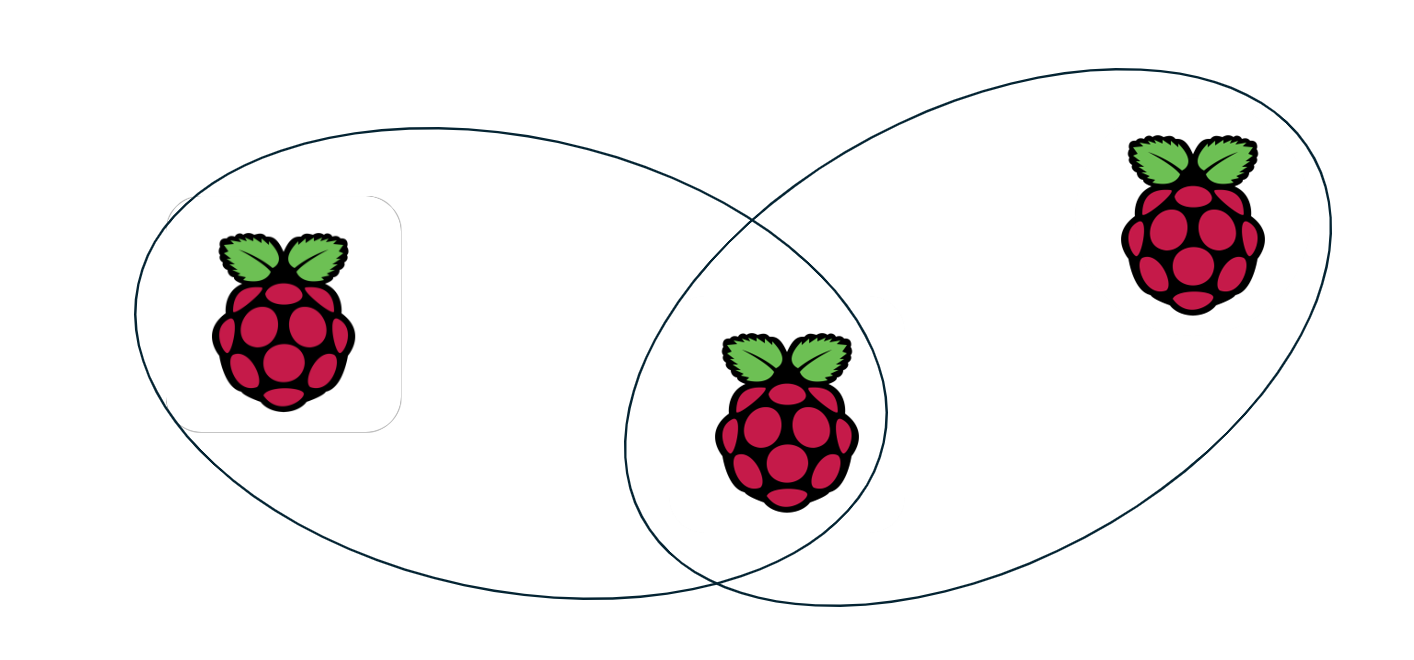
\includegraphics[scale=0.4]{image/Adhoc.png} % Include image with scale
\caption{Example of a simple ad-hoc network with three participating nodes}
\label{fig:mesh7} % Label for referencing
\end{figure}

\chapter{Concept of Practical Implementation}
\section{AODV Routing Implementaion}
\subsection{Route Discovery Process}
Route discovery in AODV is initiated when a source node needs to establish a route to a destination node. Without centralized routing mechanisms, the source broadcasts an RREQ to its neighbors. These neighbors will propagate the RREQ further if they are not the destination node. This process ensures that route discovery is efficient in decentralized environments.
\subsubsection{RREQ Packet Format and Creation}
The implementation follows the standard RREQ packet format (Figure 5.1) with some modifications (Figure 5.2). The RREQ packet is a crucial component of the route discovery process, which begins with the creation of an RREQ object using the RouteRequestMessage class.
\\
\\
The RREQ packet consists of the following fields:
\begin{itemize}
    \item Node IP Address: Identifies the originator of the RREQ.
    \item Sequence Number: Ensures that the information is fresh.
    \item Destination IP Address: Specifies the target node to which the route is being established.
    \item Destination Sequence Number: Helps to ensure that the most recent route is selected.
    \item Request ID: A unique identifier for the RREQ message.
    \item Time-to-Live (TTL): Prevents RREQs from cycling endlessly within the network.
    \item Hop Count: The number of hops from the Originator IP Address to the node handling the request.
\end{itemize}
The fields listed above are implemented in the RouteRequestMessage class, which encapsulates these attributes and provides methods for processing, validation, and propagation of the RREQ. The RREQ object is instantiated using the class constructor, as shown in Listing 5.1.
\lstset{
  basicstyle=\ttfamily\small,  % Font size and type
  numbers=left,               % Line numbers on the left
  numberstyle=\tiny,          % Font size for line numbers
  stepnumber=1,               % Line number step
  numbersep=5pt,              % Space between code and line numbers
  showstringspaces=false,     % Don't show spaces in strings
  frame=single,               % Add a frame around the code
  breaklines=true,            % Allow line breaking
  captionpos=b,               % Position of the caption (b=bottom, t=top)
  language=Python             % Programming language
}
\begin{lstlisting}[caption={RREQ Creation}, label={lst:example}]
rreq = RouteRequestMessage(req_id, node_ip, seq_no, dest_ip, dest_seq, hops, flag, ttl)

\end{lstlisting}




\begin{figure}[h]
    \centering
\begin{verbatim}
0                   1                   2                   3
    0 1 2 3 4 5 6 7 8 9 0 1 2 3 4 5 6 7 8 9 0 1 2 3 4 5 6 7 8 9 0 1
   +-+-+-+-+-+-+-+-+-+-+-+-+-+-+-+-+-+-+-+-+-+-+-+-+-+-+-+-+-+-+-+-+
   |     Type      |J|R|G|D|U|   Reserved          |   Hop Count   |
   +-+-+-+-+-+-+-+-+-+-+-+-+-+-+-+-+-+-+-+-+-+-+-+-+-+-+-+-+-+-+-+-+
   |                            RREQ ID                            |
   +-+-+-+-+-+-+-+-+-+-+-+-+-+-+-+-+-+-+-+-+-+-+-+-+-+-+-+-+-+-+-+-+
   |                    Destination IP Address                     |
   +-+-+-+-+-+-+-+-+-+-+-+-+-+-+-+-+-+-+-+-+-+-+-+-+-+-+-+-+-+-+-+-+
   |                  Destination Sequence Number                  |
   +-+-+-+-+-+-+-+-+-+-+-+-+-+-+-+-+-+-+-+-+-+-+-+-+-+-+-+-+-+-+-+-+
   |                    Originator IP Address                      |
   +-+-+-+-+-+-+-+-+-+-+-+-+-+-+-+-+-+-+-+-+-+-+-+-+-+-+-+-+-+-+-+-+
   |                  Originator Sequence Number                   |
   +-+-+-+-+-+-+-+-+-+-+-+-+-+-+-+-+-+-+-+-+-+-+-+-+-+-+-+-+-+-+-+-+
 
\end{verbatim}
\caption{Standard RREQ packet format}
\end{figure}

\clearpage
\begin{figure}[h]
    \centering
    \begin{verbatim}
0                   1                   2                   3
    0 1 2 3 4 5 6 7 8 9 0 1 2 3 4 5 6 7 8 9 0 1 2 3 4 5 6 7 8 9 0 1
   +-+-+-+-+-+-+-+-+-+-+-+-+-+-+-+-+-+-+-+-+-+-+-+-+-+-+-+-+-+-+-+-+
   |                       RREQ ID                                 |
   +-+-+-+-+-+-+-+-+-+-+-+-+-+-+-+-+-+-+-+-+-+-+-+-+-+-+-+-+-+-+-+-+
   |                 Originator IP Address                         |
   +-+-+-+-+-+-+-+-+-+-+-+-+-+-+-+-+-+-+-+-+-+-+-+-+-+-+-+-+-+-+-+-+
   |               Originator Sequence Number                      |
   +-+-+-+-+-+-+-+-+-+-+-+-+-+-+-+-+-+-+-+-+-+-+-+-+-+-+-+-+-+-+-+-+
   |                Destination IP Address                         |
   +-+-+-+-+-+-+-+-+-+-+-+-+-+-+-+-+-+-+-+-+-+-+-+-+-+-+-+-+-+-+-+-+
   |               Destination Sequence Number                     |
   +-+-+-+-+-+-+-+-+-+-+-+-+-+-+-+-+-+-+-+-+-+-+-+-+-+-+-+-+-+-+-+-+
   |                        Hop Count                              |
   +-+-+-+-+-+-+-+-+-+-+-+-+-+-+-+-+-+-+-+-+-+-+-+-+-+-+-+-+-+-+-+-+
   |                         flag                                  |
   +-+-+-+-+-+-+-+-+-+-+-+-+-+-+-+-+-+-+-+-+-+-+-+-+-+-+-+-+-+-+-+-+
   |                          TTL                                  |
   +-+-+-+-+-+-+-+-+-+-+-+-+-+-+-+-+-+-+-+-+-+-+-+-+-+-+-+-+-+-+-+-+
    \end{verbatim}
    \caption{Modified RREQ packet format}
\end{figure}

\subsubsection{RREQ Creation and Broadcasting}
{\large Broadcasting the RREQ }\\ \\
Once the RREQ is created , it is serialized and  broadcasted to neighboring nodes using the send\_rreq\_broadcast function. A User Datagram Protocol (UDP) socket is used for broadcasting, configured as shown below:
\lstset{
  basicstyle=\ttfamily\small,  % Font size and type
  numbers=left,               % Line numbers on the left
  numberstyle=\tiny,          % Font size for line numbers
  stepnumber=1,               % Line number step
  numbersep=5pt,              % Space between code and line numbers
  showstringspaces=false,     % Don't show spaces in strings
  frame=single,               % Add a frame around the code
  breaklines=true,            % Allow line breaking
  captionpos=b,               % Position of the caption (b=bottom, t=top)
  language=Python             % Programming language
}
\begin{lstlisting}[caption={RREQ Broadcasting}, label={lst:example}]
def send_rreq_broadcast(self,rreq):
       rreq.hops +=1
       id = rreq.req_id
       next_hop_bytes = socket.inet_aton(self.NodeIP)
       message_r=rreq.serialize()
          
       message_r+=next_hop_bytes
       sock = socket.socket(socket.AF_INET, socket.SOCK_DGRAM)
       sock.setsockopt(socket.SOL_SOCKET, socket.SO_BROADCAST, 1)
       broadcast_address = "192.168.1.255"
       try:
       
           sock.sendto(message_r, (broadcast_address, 50001))
           print("the route request is sent ",message_r)
       finally:
       
          # Close the socket
           sock.close()


\end{lstlisting}

Broadcasting occurs on ports above 1024 (e.g., 192.168.1.255) to avoid conflicts with privileged ports on Unix-based systems.\\

{\large Receiving and Processing the RREQ }\\ 

Each node listens for incoming RREQs on the same port used for broadcasting by binding to 0.0.0.0, allowing it to accept packets from any interface. Upon receiving an RREQ, the node deserializes the packet and performs the following actions:

\begin{enumerate}
    \item If the node is not the destination:
    \begin{itemize}
        \item The RREQ is rebroadcasted using the send\_rreq\_broadcast function, incrementing the Hop Count and decreasing the TTL.
    \end{itemize}
    \item If the node is the destination:
    \begin{itemize}
        \item A Route Reply (RREP) is generated and sent back to the source node that initiated the RREQ. This marks the beginning of the route establishment process.

    \end{itemize}
\end{enumerate}



\subsubsection{Network Considerations}
The AODV routing protocol is designed to function in decentralized, dynamic environments such as MANETs. In these environments, nodes may frequently join, leave, or move, making it challenging to maintain traditional centralized routing mechanisms. AODV, therefore, requires a connectionless communication protocol that can handle this dynamic nature without the overhead of maintaining persistent connections. This is where UDP comes into play.\\\\
{\large  \textbf{UDP Protocol}}
\begin{enumerate}
    \item \textbf{Connectionless Protocol:}AODV operates in environments where nodes can appear and disappear unpredictably. UDP does not require the establishment of a connection or the maintenance of any session state, which makes it ideal for AODV. AODV's route discovery process can send and receive packets without waiting for handshakes, keeping the communication overhead minimal.
    \item \textbf{Lightweight and Efficient:} UDP is a lightweight protocol, offering faster packet transmission with minimal overhead. Unlike Transmission Control Protocol (TCP), which requires acknowledgment of each packet and may cause delays due to retransmissions, UDP allows AODV to broadcast RREQs and replies RREPs quickly across the network.
    \item \textbf{Broadcast and Unicast Support:} AODV requires both broadcasting and unicasting. UDP supports both modes of communication easily and efficiently.
    \item \textbf{Minimal Packet Handling:} AODV nodes need to handle packets with minimal processing. UDP’s nature ensures that there is no need for error correction or packet ordering, which makes it easier for nodes to quickly forward or process the Route Request and Reply packets.
    
    
\end{enumerate}



\subsection{Route Reply}
The Route Reply (RREP) is generated and transmitted in response to a successfully processed RREQ. The destination node creates and sends the RREP back to the source node, establishing a route for data transmission.
\subsubsection{RREP Packet Format and Creation}
The RREP packet follows the standard format (Figure 5.3) with slight modifications in this implementation (Figure 5.4). The RREP is represented as an object of the class RouteReplyMessage, which encapsulates the necessary fields and methods for creating the packet.

The RREP packet consists of the following fields:
\begin{itemize}
    \item Node IP Address: Identifies the originator of the RREP.
    \item Sequence Number: can be used as the last known destination sequence number, allowing other nodes to build or update routes to the RREP's destination node, ensuring consistency and freshness in the routing table.
    \item Destination IP Address: Indicates the intended recipient of the RREP.
    \item Destination Sequence Number: The destination sequence number in the RREP is the same as the originator sequence number in the RREQ when the RREP is generated by the destination node, ensuring the originator receives the freshest sequence number for the destination.
    \item TTL: The TTL field in the RREP limits the number of hops the reply can traverse, preventing routing loops
    \item Hop Count: The number of hops from the Originator IP Address to the Destination IP Address.
\end{itemize}
The RREP packet is encapsulated in the RouteReplyMessage class, which provides methods for serialization. The object is instantiated using the class constructor, as shown below:

\lstset{
  basicstyle=\ttfamily\small,  % Font size and type
  numbers=left,               % Line numbers on the left
  numberstyle=\tiny,          % Font size for line numbers
  stepnumber=1,               % Line number step
  numbersep=5pt,              % Space between code and line numbers
  showstringspaces=false,     % Don't show spaces in strings
  frame=single,               % Add a frame around the code
  breaklines=true,            % Allow line breaking
  captionpos=b,               % Position of the caption (b=bottom, t=top)
  language=Python             % Programming language
}
\begin{lstlisting}[caption={RREQ Creation}, label={lst:example}]
rrep = RouteReplyMessage(NodeIP, seq_no, dest_ip, dest_seq, TTL, hops)

\end{lstlisting}



\begin{figure}[h]
    \centering
\begin{verbatim}
 0                   1                   2                   3
    0 1 2 3 4 5 6 7 8 9 0 1 2 3 4 5 6 7 8 9 0 1 2 3 4 5 6 7 8 9 0 1
   +-+-+-+-+-+-+-+-+-+-+-+-+-+-+-+-+-+-+-+-+-+-+-+-+-+-+-+-+-+-+-+-+
   |     Type      |R|A|    Reserved     |Prefix Sz|   Hop Count   |
   +-+-+-+-+-+-+-+-+-+-+-+-+-+-+-+-+-+-+-+-+-+-+-+-+-+-+-+-+-+-+-+-+
   |                     Destination IP address                    |
   +-+-+-+-+-+-+-+-+-+-+-+-+-+-+-+-+-+-+-+-+-+-+-+-+-+-+-+-+-+-+-+-+
   |                  Destination Sequence Number                  |
   +-+-+-+-+-+-+-+-+-+-+-+-+-+-+-+-+-+-+-+-+-+-+-+-+-+-+-+-+-+-+-+-+
   |                    Originator IP address                      |
   +-+-+-+-+-+-+-+-+-+-+-+-+-+-+-+-+-+-+-+-+-+-+-+-+-+-+-+-+-+-+-+-+
   |                           Lifetime                            |
   +-+-+-+-+-+-+-+-+-+-+-+-+-+-+-+-+-+-+-+-+-+-+-+-+-+-+-+-+-+-+-+-+
 
\end{verbatim}
\caption{Packet Format Description}
\end{figure}
\clearpage



\begin{figure}[h]
    \centering
    \begin{verbatim}
0                   1                   2                   3
    0 1 2 3 4 5 6 7 8 9 0 1 2 3 4 5 6 7 8 9 0 1 2 3 4 5 6 7 8 9 0 1
   +-+-+-+-+-+-+-+-+-+-+-+-+-+-+-+-+-+-+-+-+-+-+-+-+-+-+-+-+-+-+-+-+
   |                           TTL                                 |
   +-+-+-+-+-+-+-+-+-+-+-+-+-+-+-+-+-+-+-+-+-+-+-+-+-+-+-+-+-+-+-+-+
   |                    Originator IP Address                      |
   +-+-+-+-+-+-+-+-+-+-+-+-+-+-+-+-+-+-+-+-+-+-+-+-+-+-+-+-+-+-+-+-+
   |                  Originator Sequence Number                   |
   +-+-+-+-+-+-+-+-+-+-+-+-+-+-+-+-+-+-+-+-+-+-+-+-+-+-+-+-+-+-+-+-+
   |                    Destination IP Address                     |
   +-+-+-+-+-+-+-+-+-+-+-+-+-+-+-+-+-+-+-+-+-+-+-+-+-+-+-+-+-+-+-+-+
   |                  Destination Sequence Number                  |
   +-+-+-+-+-+-+-+-+-+-+-+-+-+-+-+-+-+-+-+-+-+-+-+-+-+-+-+-+-+-+-+-+
   |                           Hop Count                           |
   +-+-+-+-+-+-+-+-+-+-+-+-+-+-+-+-+-+-+-+-+-+-+-+-+-+-+-+-+-+-+-+-+
    \end{verbatim}
    \caption{RREP Packet Format}
\end{figure}


\subsubsection{Sending the RREP}

After constructing the RREP, the destination node sends it to the source node using a UDP socket. This process is handled by the send\_rrep function , which serializes the RREP object and transmits it to the next hop along the route.\\
\\
Key Steps in Sending the RREP:
\begin{enumerate}
    \item Serialization of the RREP in the send\_rrep function is performed using the serialize\_1 method of the RouteReplyMessage class, as demonstrated in the following code snippets:

    \lstset{
  basicstyle=\ttfamily\small,  % Font size and type
  numbers=left,               % Line numbers on the left
  numberstyle=\tiny,          % Font size for line numbers
  stepnumber=1,               % Line number step
  numbersep=5pt,              % Space between code and line numbers
  showstringspaces=false,     % Don't show spaces in strings
  frame=single,               % Add a frame around the code
  breaklines=true,            % Allow line breaking
  captionpos=b,               % Position of the caption (b=bottom, t=top)
  language=Python             % Programming language
}
\begin{lstlisting}[caption={Serializing the RREP Instance }, label={lst:example}]
 message = rrep.serialize_1() 
\end{lstlisting}
\clearpage
\begin{lstlisting}[caption={Serialization of the RREP Function}, label={lst:example}]
def serialize_1(self):
        # Convert IP addresses to bytes
        node_ip_bytes = socket.inet_aton(self.NodeIP)
        dest_ip_bytes = socket.inet_aton(self.dest_ip)
        
        message = struct.pack("!I4sI4sIII", self.rep_id,node_ip_bytes, self.seq_no, dest_ip_bytes, self.dest_seq, self.TTL, self.hops)
        
        return message
\end{lstlisting}
    \item Identify the next hop using the routing table using the following function:
    \begin{lstlisting}[caption={Serialization of the RREP Function}, label={lst:example}]
def lookup_2(self, dest_ip):
        if dest_ip in self.table:
            return self.table[dest_ip]['next_hop']
        else:
            return None
\end{lstlisting}
    \item Send the serialized packet to the next hop’s IP address and port like the following code snippet show :
   \begin{lstlisting}[caption={Serialization of the RREP Function}, label={lst:example}]
        sock = socket.socket(socket.AF_INET, socket.SOCK_DGRAM)
        dest_port = 50002
        sock.sendto(message, (next_hop, dest_port))
\end{lstlisting}
   
\end{enumerate}
\subsubsection{Receiving and Forwarding the RREP}
Each node along the route monitors the same UDP port used for transmitting the RREP in order to receive incoming RREP messages. Upon receiving an RREP:
\begin{enumerate}
    \item Intermediate Nodes:
    \begin{itemize}
        \item Update the routing table with the reverse path from the RREP.
        \item  Increment the hop count.
        \item Forwarding the RREP to the Next Hop Based on the Routing Table
    \end{itemize}
    \item Destination Node:
    \begin{itemize}
        \item If the node is the intended destination, the RREP marks the completion of the route discovery process.
        \item The source node uses the route for data transmission.
    \end{itemize}
    
\end{enumerate}





\begin{algorithm}
\caption{Receive Route Reply }
\begin{algorithmic}[1]
\REQUIRE Routing table (\textit{table}), Node's IP address (\textit{NodeIP})
\STATE Initialize a UDP socket (\textit{sock}) bound to IP \texttt{192.168.1.3} and port \texttt{50002}.
\STATE Enable socket broadcast option.
\WHILE{True}
    \STATE Set a timeout of 2 seconds.
    \IF{Message is available on the socket within the timeout period}
        \STATE Read the RREP message and sender's address.
        \STATE Unpack the RREP message into:
        \STATE \hspace{1em} \textit{rep\_id}: Route Reply ID
        \STATE \hspace{1em} \textit{node\_ip}: Sender's IP
        \STATE \hspace{1em} \textit{hop\_count}: Hop count
        \STATE \hspace{1em} \textit{dest\_ip}: Destination IP
        \STATE \hspace{1em} \textit{next\_hop}: Next hop IP
        \STATE Add a route to the routing table with the extracted information.
        \STATE Display the updated routing table.
        \IF{\textit{dest\_ip} matches the current node's IP (\textit{NodeIP})}
            \STATE Generate a data packet (\textit{packet}) for \textit{dest\_ip} via \textit{node\_ip}.
            \STATE Start a thread to send the data packet.
        \ELSE
            \STATE Log a message indicating forwarding of the RREP.
            \STATE Create a new RREP message object (\textit{rrep}) with the unpacked data.
            \STATE Lookup the next hop for \textit{dest\_ip} in the routing table.
            \STATE Log the next hop information.
            \STATE Start a thread to forward the RREP message to the next hop.
        \ENDIF
    \ENDIF
\ENDWHILE
\end{algorithmic}
\end{algorithm}

\clearpage

\subsection{Threading in the AODV Implementation}
Threading is fundamental to the efficiency and responsiveness of our AODV  routing protocol implementation. This is because the protocol involves multiple tasks, such as sending and receiving messages, that need to be managed concurrently. Threads provide lightweight, parallel flows of execution within a process, enabling the simultaneous handling of tasks. Network protocols, including AODV, leverage threads to handle network events like message reception and forwarding concurrently.
\subsubsection{Thread Management in AODV}
Each node operates three primary threads running in the background:
\begin{enumerate}
    \item RREQ Thread: Handles the reception and processing of RREQ messages.
    \item RREP Thread: Manages the reception and processing of RREP messages.
    \item Data Packet Thread: Processes incoming data packets.
\end{enumerate}

These threads are created using the threading.Thread class with the following structure:
 \begin{lstlisting}[caption={Thread Creation in Python}, label={lst:example}]
threading.Thread(target=function_name, args=())
\end{lstlisting}
\begin{itemize}
    \item Target: The function that the thread will execute.
    \item Args: The parameters passed to the target function.
\end{itemize}
\subsubsection{Thread Lifecycle and Behavior}
Each thread is designed to run continuously, using an infinite loop to remain in a listening state. The process flow is as follows:
\begin{enumerate}
    \item Receiving Messages: When an RREQ, RREP, or data packet is received, the corresponding thread processes the message.
    \item Forwarding Messages: A new thread is spawned to forward the message to the next hop in the network.
\end{enumerate}
\subsubsection{Special Cases for Thread Creation}
\begin{itemize}
    \item Destination Node Handling RREQ: When an RREQ is received at the destination node, a new thread is started to send an RREP back to the source.
    \item Destination Node Handling RREP: Upon receiving an RREP at the destination node, another thread is initiated to handle data packet transmission.
\end{itemize}
\subsubsection{Interaction Between Threads}
To clarify the interaction between threads in the system, the following sequence diagram illustrates the process:

\begin{figure}[h]
\graphicspath{{/image/}} % Directory path for images
\centering
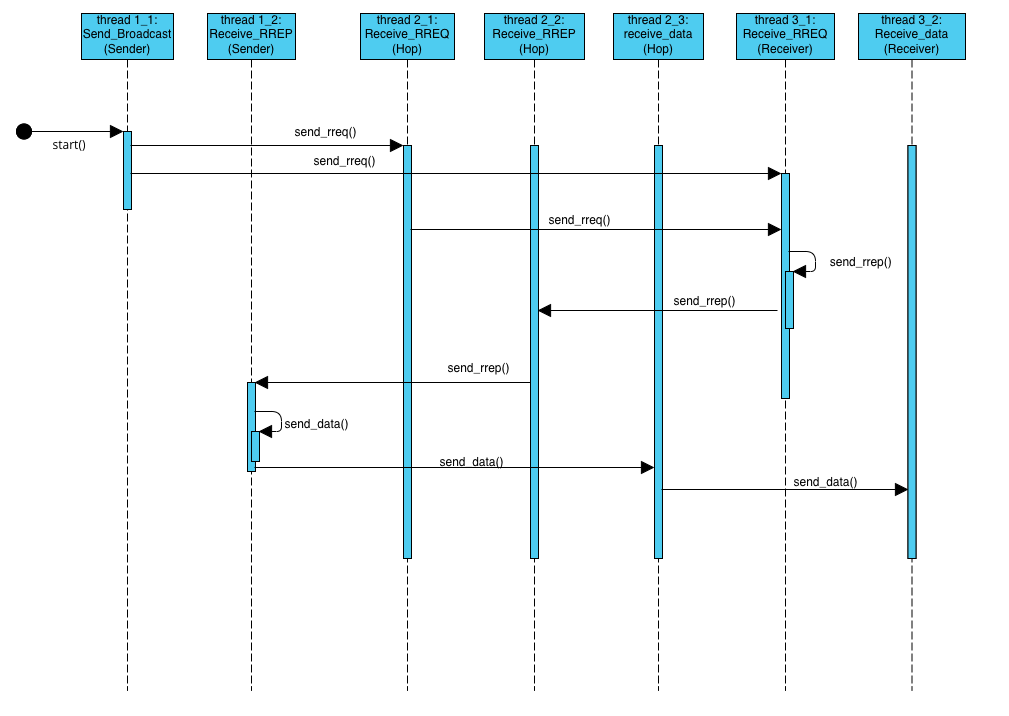
\includegraphics[scale=0.3]{image/sequencediagramm.png} % Include image with scale
\caption{Thread Management and Message Flow in AODV Routing Protocol}
\label{fig:mesh9} % Label for referencing
\end{figure}

The AODV process, as shown in the sequence diagram, starts with the broadcasting of a Route Request. Node 2 and Node 3 receive this RREQ by threads 2\_1 and 3\_1, respectively. In this case, Node 2 is not the destination, so it rebroadcasts the RREQ. Node 3, after receiving the RREQ by thread 3\_1, creates another thread to send a unicast Route Reply back to the source.

Node 2 receives the RREP via thread 2\_2. Since Node 2 is not the intended destination, it forwards the RREP to Node 1, which processes it via thread 1\_2. Further, upon receiving the RREP, Node 1 creates a new thread for the transmission of data. This data is received by Node 2 through thread 2\_3 and is further forwarded to Node 3 for processing via thread 3\_2.

Note that Node 2 creates various threads to forward the RREQ, RREP, or even data packets. For example, when receiving the RREQ, Node 2 sends out a thread that rebroadcasts this RREQ packet. Also, in the event of receiving the RREP and a DATA packet, respectively, Node 2 will launch threads with the ultimate goal of further forwarding these seamlessly across the network.



\subsection{AODV Routing Protocol and Routing Table Management}
AODV  is a routing protocol responsible for managing the routing table, which stores route information. These routes are extracted from the control packets of the AODV protocol, such as Route Requests (RREQs) and Route Replies (RREPs). Each entry in the AODV routing table contains the following fields:
\begin{itemize}
    \item Destination IP Address
    \item Destination Sequence Number
    \item Hop Count
    \item Next Hop
    \item Lifetime
\end{itemize}
\subsubsection{Populating Routing Table Fields}
The fields of the routing table are populated as follows:
\begin{itemize}
    \item Most fields, such as Destination IP Address, Destination Sequence Number, and Hop Count, are extracted from the received RREQ and RREP packets.
    
    \item The Lifetime field is set to a constant value (120 seconds) across all nodes.
\end{itemize}
\lstset{
  basicstyle=\ttfamily\small,  % Font size and type
  numbers=left,               % Line numbers on the left
  numberstyle=\tiny,          % Font size for line numbers
  stepnumber=1,               % Line number step
  numbersep=5pt,              % Space between code and line numbers
  showstringspaces=false,     % Don't show spaces in strings
  frame=single,               % Add a frame around the code
  breaklines=true,            % Allow line breaking
  captionpos=b,               % Position of the caption (b=bottom, t=top)
  language=Python             % Programming language
}
\begin{lstlisting}[caption={Populating Routing Table Fields Code}, label={lst:example}]
unpacked_data = struct.unpack("!I4sI4sIII4s", rrep_msg)
node_ip=socket.inet_ntoa(unpacked_data[1])
next_hop=socket.inet_ntoa(rrep_msg[-4:])
rep_id=unpacked_data[0]
dest_ip = socket.inet_ntoa(unpacked_data[3])
# adding the route with a lifetime equal 120 s
table.add_route(node_ip,next_hop,unpacked_data[6],
unpacked_data[2],120)
\end{lstlisting}
\subsubsection{Reverse Path Mechanism}
The AODV protocol relies on a Reverse Path Mechanism to establish efficient bidirectional communication during routing. This mechanism dynamically creates reverse routes while processing RREQs and RREPs, enabling seamless data transmission.\\\\
{\large Handling RREQ and RREP Packets}
\\
When a RREQ is generated by a source node or forwarded by an intermediate node, each node adds its IP address as the Next Hop in the RREQ packet. This process enables every node along the path to register a reverse route back to the source node. The reverse path ensures that when the RREP is forwarded back, it efficiently reaches the correct destination (the source of the RREQ). The implementation of this process in Python is demonstrated below:

\lstset{
  basicstyle=\ttfamily\small,  % Font size and type
  numbers=left,               % Line numbers on the left
  numberstyle=\tiny,          % Font size for line numbers
  stepnumber=1,               % Line number step
  numbersep=5pt,              % Space between code and line numbers
  showstringspaces=false,     % Don't show spaces in strings
  frame=single,               % Add a frame around the code
  breaklines=true,            % Allow line breaking
  captionpos=b,               % Position of the caption (b=bottom, t=top)
  language=Python             % Programming language
}
\begin{lstlisting}[caption={Python code adding the Next Hop to an RREQ packet}, label={lst:example}]
next_hop_bytes = socket.inet_aton(self.NodeIP)
message_r+=next_hop_bytes
\end{lstlisting} 
For RREP packets, a similar reverse path mechanism is employed. Each node links the source or intermediate node's IP address as the Next Hop in its routing table. This mechanism ensures that data packets can flow seamlessly in both directions: from the source node (RREQ initiator) to the destination node (RREP sender) and from the destination node back to the source node for data transmission.
\subsubsection{Data Structure for the Routing Table}
The routing table is represented as a list, with each entry being a dictionary that contains the specified fields. Each node maintains its own routing table, implemented as an object of the RoutingTable class, and new routes are added using the add\_route function provided by the class.

\begin{lstlisting}[caption={Python code for the add\_route function}, label={lst:add_route}]
def add_route(self, destination, next_hop, hop_count, dest_sequence_number, TTL):
    route = {"destination": destination,
             'next_hop': next_hop,
             'hop_count': hop_count,
             'dest_sequence_number': dest_sequence_number,
             'TTL': TTL
            }
    self.table.append(route)
\end{lstlisting}

\subsection{Ad-hoc Mode Configuration in AODV}
Adhoc Mode is the basic setup needed to use the AODV protocol in this project. In real-life situations Ad-hoc Mode allows devices to communicate directly with each other. They don't need a central system like routers or access points to connect. This decentralized structure is important for enabling flexible routing when nodes move around or the layout changes often.

For this implementation, the Raspi devices are configured to operate in Ad-hoc mode, enabling them to create a network for communication rather than connecting to existing Wi-Fi networks. By default, RPi devices connect to Wi-Fi routers by searching for available SSIDs. However, in Ad-hoc mode, we manually assign the SSID and IP address to each device. The Raspi will create its network, named RPitest, and communicate within this network. The Ad-hoc mode configuration on the RPi is set by editing the /etc/network/adhoc-interface file, which defines the static IP address (e.g., 192.168.1.1), subnet mask (255.255.255.0), and wireless channel (4), ensuring that all nodes in the network are on the same channel and SSID. This setup is essential for the nodes to communicate with each other, as they must operate on the same SSID and wireless channel\cite{pyshine2025}. Based on empirical testing, I observed that if the nodes are configured with different SSIDs or channels, they cannot ping each other, which is a critical factor for successful communication in Ad-hoc mode.

This configuration allows the nodes to recognize and ping each other, ensuring seamless communication in the Ad-hoc setup. Additionally, a DHCP server is configured to assign IP addresses to new devices connecting to the network. For example, new devices will receive IP addresses starting from 192.168.1.5. The setup further ensures that after each reboot, the Raspi automatically follows the Ad-hoc interface settings, creating a network that other devices can join.

The Raspi devices use this configuration to exchange RREQ and RREP messages, allowing the AODV protocol to dynamically establish and maintain routes. The Ad-hoc network configuration is essential to the operation of the AODV protocol, as it supports both broadcast and unicast communication required for route discovery and data forwarding.
\section{Forwarding Towards Underwater}
\subsection{Handling Route Request Timeout}
When a node is underwater, a route request intended for an underwater destination node is sent out by broadcast. If no route reply is received within a timeout of 2 seconds, a timeout event is triggered. To handle this efficiently, the select module is used to monitor the readability of the socket. This avoids blocking operations and ensures the system remains responsive.

The select.select function waits for incoming data or connection events on monitored sockets, and based on the event, the system decides how to proceed. This functionality is implemented in the rec\_rrep function, where timeouts are managed and appropriate actions are taken.

\begin{lstlisting}[caption={Route Request Timeout}, label={lst:example}]
def rec_rrep(self,table,NodeIP,destination_ip) :
    timeout = 2  # 2 seconds
    readable, _, _ = select.select([sock], [], [], timeout)
    if readable:
        reep_Processing()
    else:
        relayreq_send()
\end{lstlisting}
In this code, if the socket is readable within the timeout period, the system proceeds with processing the RREP; otherwise, it sends a relay request.
\subsubsection{Relay Request Handling}
The relay request has the same structure as the route request but is broadcast to the address 192.168.1.255. The key difference lies in the use of different ports for broadcasting and receiving, which is handled by the rec\_relay\_request() function.

In this function, only the gateways respond to the relay request with a unicasted message back to the source of the relay request. This helps the system manage the relay mechanism efficiently.


\begin{lstlisting}[caption={Relay Request Handling}, label={lst:example}]
def rec_relay_request(self,table):
    if self.Node_type=="G":
       relay_request_Processing()
       relay_reply_send()
    else:
       relay_request_forwarding()
       
\end{lstlisting}
\subsubsection{Relay Reply Structure}
The structure of the relay reply is the same as the route reply, with the additional information of the gateway's coordinates. When a gateway responds to a relay request, it also includes its coordinates, which are registered in the mission table (usv\_table) on the sender node. The usv\_table has the following fields:
\begin{itemize}
    \item Destination\_Ip: the Ip adresse of the underwater destination node
    \item Source\_Ip: The Ip adresse of the Gateway that sended the relay reply
    \item coord\_x: The x Coordination of the Gateway
    \item coord\_y: The y Coordination of the Gateway
    \item coord\_z: The z Coordination of the Gateway
    \item Distance: The euclidean distance between the under water node and the gateway nodes
\end{itemize}  
In this case, the coordinates of underwater nodes are provided by the source node in its Constructor.


\subsubsection{Gateway Interfaces}
To enable communication between the gateway (Raspberry Pi) and the acoustic modem, an additional Ethernet interface must be configured. This interface allows the gateway to establish a TCP connection with the acoustic modem while operating in Ad-hoc mode for the wireless network.\\\\
The configuration can be achieved using one of the following methods:
\begin{enumerate}
    \item \textbf{Manual Configuration via Terminal}\\
     The Ethernet interface can be configured manually each time the system starts by executing the following command in the terminal:
\begin{lstlisting}
$ sudo ifconfig eth0 172.18.1.x netmask 255.255.255.0 
\end{lstlisting}
\item \textbf{Automatic Configuration via rc.local}\\
To avoid manual setup after each startup, the Ethernet interface configuration can be added to the rc.local file. This file is executed by the system after all standard services have started.

Steps to configure via rc.local:
\begin{itemize}
    \item Open the rc.local file:
    \begin{lstlisting}
$sudo nano /etc/rc.local
\end{lstlisting}
    \item Open the rc.local file:
    \begin{lstlisting}
$ sudo ifconfig eth0 172.18.1.x netmask 255.255.255.0 &
# The ‘&’ ensures the command runs in the background

\end{lstlisting}
\end{itemize}

\end{enumerate}



\subsubsection{Establishing TCP Connection with the Acoustic Modem}
After configuring the Ethernet interface, the next step is to establish a TCP connection to send data to the underwater network. The following Python code snippet demonstrates creating and establishing a TCP connection to the acoustic modem:
\begin{lstlisting}
sock = socket.socket(socket.AF_INET, socket.SOCK_STREAM)
sock.connect(("172.18.1.110", 9200)) 
\end{lstlisting}
This code creates a TCP socket and connects to the acoustic modem using the specified IP address (172.18.1.110) and port (9200).     
\subsubsection{Forwarding Data Underwater}
When the sender node receives relay requests from all gateways, it registers their coordinates and calculates the distance between each gateway and the underwater nodes. The sender then selects the gateway with the shortest distance to forward the data. Upon receiving the data, the gateway places it into a First-In-First-Out (FIFO) queue, where a dedicated thread processes queued data every 10 seconds. Each data packet is formatted into the acoustic\_data string, which is then converted into bytes using the .encode() method. This formatted structure includes metadata such as the data size (20), the receiver's acoustic address (2), the acknowledgment mode (ack), and the actual payload (data). The final structure is as follows: 
\begin{lstlisting}
acoustic_data="AT*SENDIM,20,2,ack,".encode()+data+ "\n".encode()
\end{lstlisting}
This formatted command is then transmitted to the acoustic modem for forwarding to the underwater node.





\chapter{Practical Setup}
This paper presents the design of a practical test environment aimed at evaluating AODV-based communication protocols in both underwater and above-water scenarios. The test setup included RasPi nodes and two acoustic modems used for facilitating underwater communication.
\section{Hardware Configuration}
\subsection{Above-Water Network}
For The Above Network there is three types Of Nodes:
\begin{itemize}
    \item The sender Node : A Raspberry Pi configured to initiate AODV route requests, simulating a node that begins the process of communication.
    
    \item The Hop Node : Two configurations of hops were tested in the above-water network:
        \begin{itemize}
            \item One Hop Test: In this setup, the Hop Node was directly in between the Sender Node and the Receiver Node, thus allowing a line of communication with just one intermediate hop. 
            \item Two Hop Test: This configuration added an additional Intermediate Hop Node, increasing the complexity of the routing path. In this setup, data from the Sender Node was first sent to the first hop, then forwarded to a second hop, before reaching the Receiver Node.
        \end{itemize}
    \item The Receiver Node: A Raspberry Pi configured to perform several functions in the AODV routing process: it receives the Route Request packet, sends the Route Reply back to the sender, and receives the data transmitted from the sender via the routing protocol through the network.
    
\end{itemize}
\begin{figure}[h!]
    \centering
    \includegraphics[width=0.7\textwidth]{image/2_hops.JPG}
    \caption{Two-Hop Test}
    \label{fig:example0}
\end{figure}

\subsection{Underwater Communication}
Communication between above-water and underwater nodes is facilitated through two acoustic modems, where data will be sent and received as acoustic waves-something pretty common for communication underwater. These modems act like a bridge for data transfer from Raspberry Pi nodes that lay above the water to an underwater node.
\subsubsection{First Acoustic Modem (Connected to the Receiver Node)}
The first acoustic modem, shown in Figure 6.2, is silver and assigned the IP address 127.18.1.110. It was connected to the Gateway Node, a Raspberry Pi, via a TCP communication link, ensuring reliable data transmission. This modem converted digital data into acoustic signals for underwater transmission, enabling seamless communication between the sender and receiver acoustic modems.
\begin{figure}[h!]
    \centering
    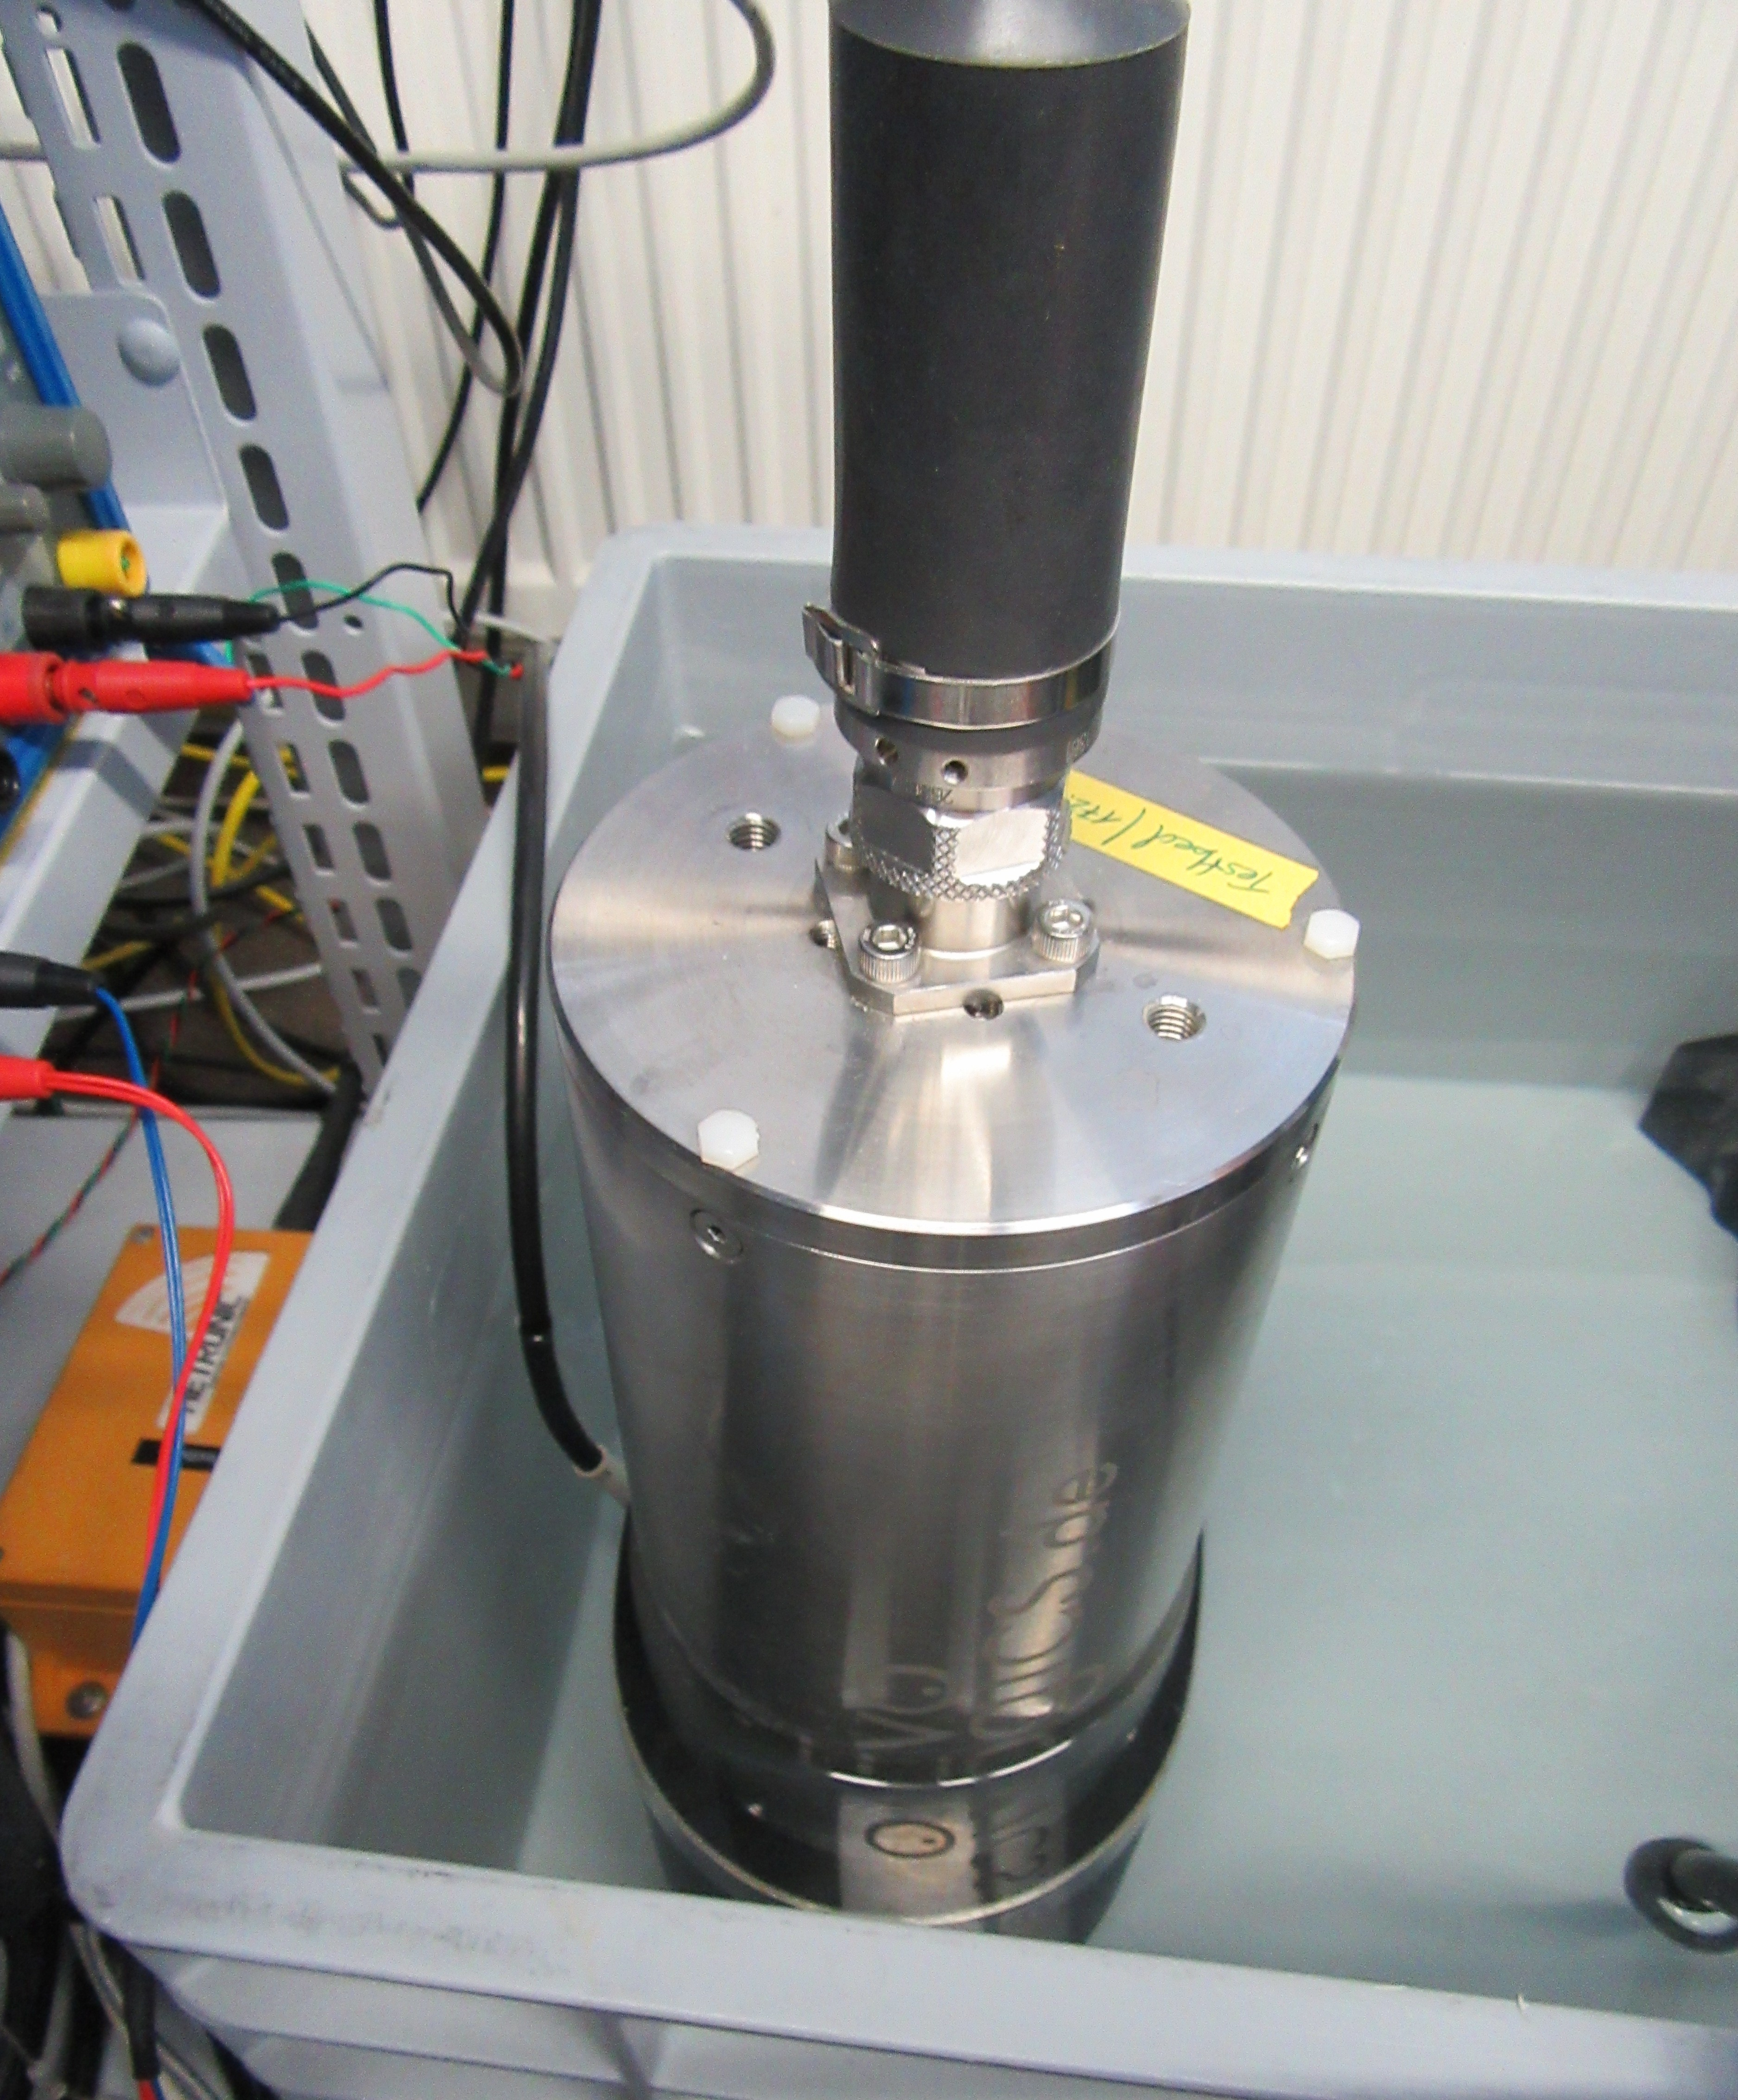
\includegraphics[width=0.5\textwidth]{image/acoustic_modem1.JPG}
    \caption{Acoustic Modem 1}
    \label{fig:example1}
\end{figure}


\subsubsection{Second Acoustic Modem (Connected to the Listener Node)}
The second acoustic modem, as shown in Figure 6.3, is colored white with an IP address of 10.201.25.10 and was submerged underwater, receiving acoustic signals from the first modem. The Listener Node, a Raspberry Pi positioned above water, was connected via a TCP connection to this second modem, which received and processed the data transmitted, verifying its integrity for accuracy. In this setup, the underwater acoustic modem was communicating with the Listener Node above the water, which in turn would take care of the data onward for processing.
\begin{figure}[h!]
    \centering
    \includegraphics[width=0.5\textwidth]{image/acoustic_modem2.JPG}
    \caption{Acoustic Modem 2}
    \label{fig:example2}
\end{figure}
\subsubsection{power supplies Of the acoustic Modem}
The power supply for the two acoustic modems was shared. Each acoustic modem is supposed to operate on 24 V with a current draw between 60 and 70 mA. This setup is pretty stable and reliable, allowing appropriate voltage and current specifications for the functioning of both modems.(See Figure 6.4)
\clearpage
\begin{figure}[h!]
    \centering
    \includegraphics[width=0.5\textwidth]{image/powersupply.JPG}
    \caption{Power Supply }
    \label{fig:example3}
\end{figure}
\subsubsection{Connection between the modem and the raspi}
As previously mentioned, the Raspberry Pi establishes a TCP connection with the acoustic modem, which is represented through an Ethernet connection. To set up this connection, we used an Ethernet cable to link the acoustic modem to a switch, and another Ethernet cable to connect the switch to the Raspberry Pi.(see Figure 6.5)
\begin{figure}[h!]
    \centering
    \includegraphics[width=0.6\textwidth]{image/Ethernet.JPG}
    \caption{Power Supply }
    \label{fig:example4}
\end{figure}

\section{Test Environment and Equipment}

\subsection{Test Location}
The entire experimental procedure was carried out in the private lake 'ATLAS Sea' of the company. It has been specifically chosen because it provides suitable conditions to simulate practical, realistic underwater acoustic communication. Due to its controlled environment, this lake creates perfect conditions for testing, with experiments conducted very close to real situations, providing very reliable results.
\begin{figure}[h!]
    \centering
    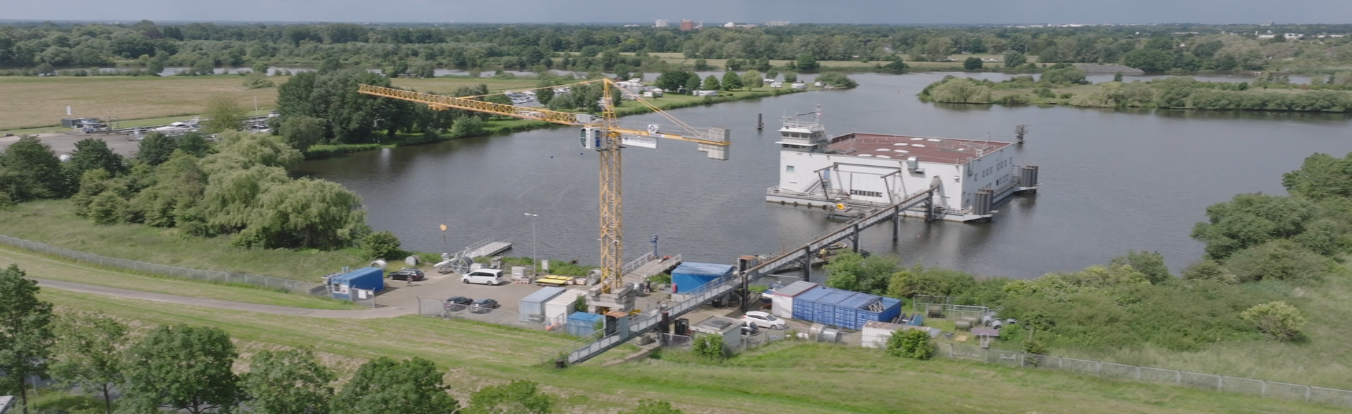
\includegraphics[width=0.9\textwidth]{image/Location.png}
    \caption{Test Location}
    \label{fig:example5}
\end{figure}
\subsection{Drone Integration}
A drone was utilized to deploy and position the Raspberry Pi nodes in both above-water and underwater environments, ensuring precise placement for the experiments. The drone played a crucial role in facilitating the mobility and efficient setup of the nodes during testing.

For the single-hop test, one drone was employed to manage the deployment of the Raspberry Pi nodes. In contrast, the two-hop test required the use of two drones to accurately position the nodes in their designated locations, ensuring optimal conditions for evaluating multi-hop communication.
\begin{figure}[h!]
    \centering
    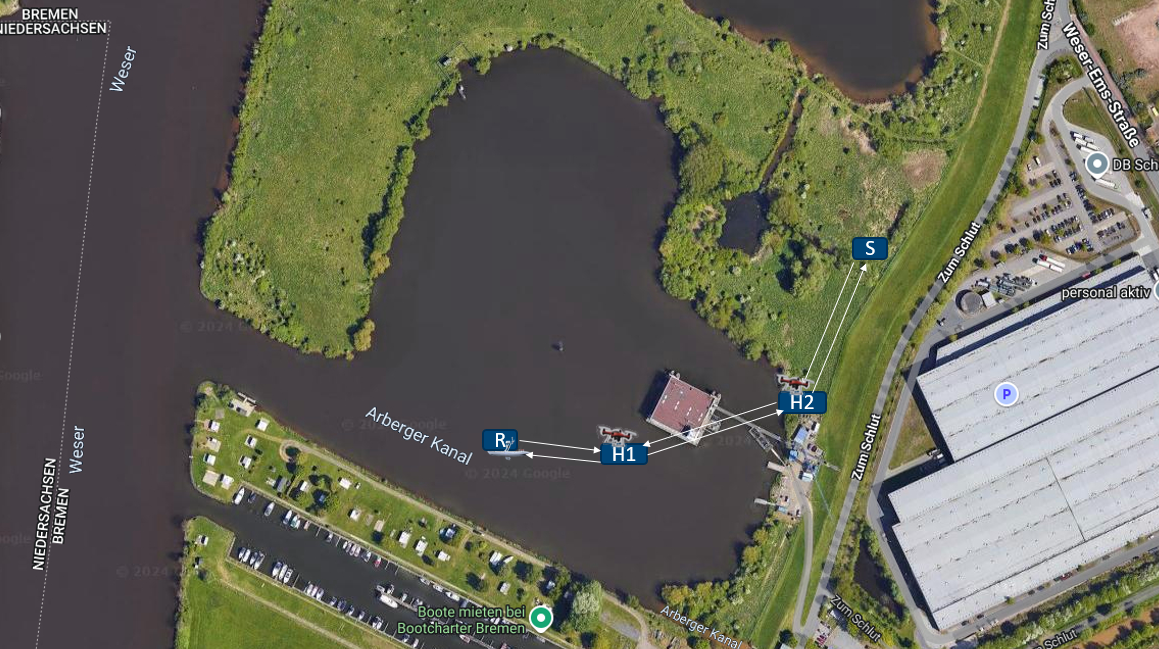
\includegraphics[width=0.7\textwidth]{image/2_Drohne_integration.png}
    \caption{Drohne Integration}
    \label{fig:example6}
\end{figure}

\subsection{Protective Enclosures}
We used custom-designed 3D-printed cases to securely attach the Raspberry Pi nodes to the drones. The cases were specifically designed to house the Raspberry Pi along with a power bank that could provide enough energy to keep the device operational throughout the testing period.

The cases were attached to the drones using strong plastic cables to hold them in place during deployment. However, considering the dynamic and possibly turbulent conditions of flying and deployment, detachment of the cases could not be ruled out. Such detachments may be facilitated by improper cable fastening, sudden movements of the drone, or even environmental challenges like strong winds.

In order to reduce these risks, extra precautions were taken during the attachment and choosing of materials that would serve best under operational conditions.
\begin{figure}[h!]
    \centering
    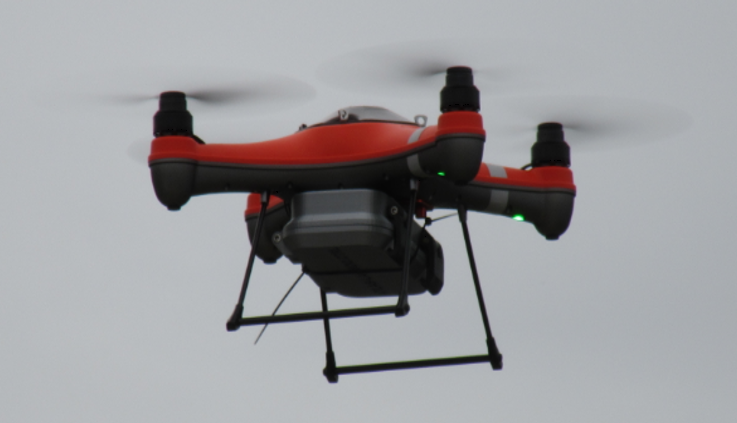
\includegraphics[width=0.6\textwidth]{image/Case_Drohne.png}
    \caption{custom-designed 3D-printed case}
    \label{fig:example7}
\end{figure}
\section{Implementation Process}
\subsection{One-Hop Test}
The one-hop test involved communication between the Sender Node and the Receiver Node, with a single hop existing between them. This scenario was tested in two configurations:
\subsubsection{One-Hop Test Without Acoustic Modem}
In this setup, the communication between the Sender Node and the Receiver Node was totally above water. The Receiver Node received the Route Request from the Sender Node and responded with a Route Reply, thus establishing a direct route for data transfer. Further, a hop Raspberry Pi attached to a drone was also deployed to simulate the potential intermediate nodes in the path. This test provided a basis for comparing the performance of the system not using the underwater network.
\subsubsection{One-Hop Test With Acoustic Modem}

In this configuration, the underwater network was integrated into the setup, with the Receiver  forwarding data via  a  silver  acoustic  modem (IP address: 127.18.1.110).
This modem transmitted the data as acoustic signals to the white acoustic modem (IP address:10.201.25.10), submerged underwater. The Listener Node, connected to the white modem via TCP, received and processed these acoustic signals. This test aimed to evaluate the performance of the underwater communication system in a one-hop scenario, focusing on key factors such as latency, data integrity, and reliability.
\begin{figure}[h!]
    \centering
    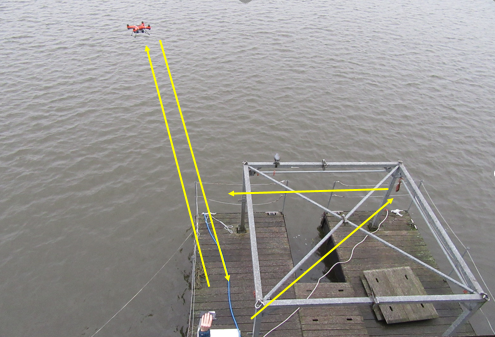
\includegraphics[width=0.7\textwidth]{image/test_with_acoustic.png}
    \caption{Test With Acoustic Modem}
    \label{fig:example8}
\end{figure}

\subsection{Two-Hop Test}
In this experiment, the performance of the AODV routing protocol was tested over a multi-hop network with two drones: one sender at our site and one receiver in Moritz. The performance evaluation was done to determine how AODV performs when distance varies, with two drones relaying the data as intermediary nodes. The tests were conducted over different distance configurations where the sender sends to the first drone, the drones send to each other, and finally, the second drone sends to the receiver. Distances between the sender, drones, and receiver were changed to test the performance of the AODV protocol. During these tests, important metrics were taken, such as route discovery time, packet delivery ratio, and end-to-end delay, regarding how effective and efficient AODV is in such multi-hop scenarios. Results derived from these tests will allow us to understand how AODV adapts in both different network configurations and varied distances between nodes.







\chapter{Results And Discussions}
This chapter provides the results of the tests done to assess how effectively the AODV protocol works when integrating above-water and underwater domains. Important objects of these experiments included comparing the normal AODV in the above-water network against the integrated system where the data will be transmitted to the underwater nodes by acoustic modems. The system performance was quantified using different metrics related to packet delivery ratio (PDR) and latency. These results are now analyzed and discussed for meaningful conclusions on the feasibility and effectiveness of the proposed system.
\section{Presentation of Results}
\subsection{Baseline AODV Performance}
\subsubsection{PDR Analysis}
PDR is calculated for the ratio of total received bytes by the receiver and total bytes sent by a sender, which includes all RREQ packets and data packets. The mean PDR observed is 83.95\%, which is interpreted as approximately 83.95\% of the forwarded packets being delivered to a receiver on average, out of which nearly 16\% of packets were undelivered or lost during transmission.

The average PDR of 83.95\% is a relatively good result, suggesting that the AODV protocol performed reliably in the network under most conditions. However, there were instances of packet loss which can be attributed to several factors, as described below:
\begin{itemize}
    \item Distance Between Nodes: The test distances considered were 250m, 350m, 450m, and 550m. With an increase in the distance between nodes, signal attenuation and interference may have occurred, further contributing to the reduction in successful forwarding of RREQs. If the distance in one hop is too big, sometimes Route Requests cannot be forwarded, which causes route discovery failure.
    \item Weak Connectivity Between Intermediate Hops: Poor connectivity between hops in a multi-hop network, where the middle nodes act as relays, leads to packet forwarding failure. The distance between the hops is an important factor. For example, longer distances of 450 and 550 meters may cause the intermediate hops to be out of reach of each other, thus not maintaining a stable connection to allow RREQ to reach its destination. This is further supported by the fact that, once the route was established successfully, data packets were delivered with 100\% reliability. Thus, the problem exists mainly in the route discovery phase and not in the data transmission phase.
    \item RREQ and  RREP Failures: One of the probable causes for packet loss in such a scenario is when, in one instance, RREQ does not reach the receiver or RREP does not reach the sender back. This could have failed because of the distance and attenuation of signals at greater distances or every hop too far apart for effective communication.
\end{itemize}


\subsubsection{RTT Analysis}
Round Trip Time (RTT) performance was measured for the AODV protocol to evaluate latency under different total distances between the sender and receiver: 250m, 350m, 450m, 550m, 650m, and 750m. The communication was facilitated by two intermediate nodes, dividing the total distance into three equal segments to mimic realistic multi-hop scenarios.
The RTT Mean vs. Distance results reveal the following trends:
\begin{enumerate}
    \item RTT Increases with Distance:
       \begin{itemize}
           \item At 250m, the mean RTT was 52.25 ms, serving as the baseline latency for the shortest tested distance.
           \item At 750m, the mean RTT rose significantly to 73.25 ms, reflecting the cumulative delays introduced by longer distances and additional hops.
       \end{itemize}
    \item Intermediate Results:
      \begin{itemize}
          \item For distances of 350m, 450m, and 550m, the mean RTTs were 49.25 ms, 50.50 ms, and 59.25 ms, respectively.

          \item At 650m, the mean RTT was 51.00 ms, slightly lower than at 550m. This unexpected result could be attributed to real-world factors such as improved signal propagation or reduced interference during the testing period.
      \end{itemize}
\end{enumerate}

The results demonstrate a predictable increase in latency as the total communication distance grows, consistent with theoretical expectations of multi-hop delays. The deviation observed at 650m, where the RTT mean was slightly lower, underscores the variability of real-world network performance, which can be influenced by environmental factors and transient network conditions.

These findings highlight the need for reliable connectivity between intermediate nodes to minimize latency and maintain stable network performance in multi-hop scenarios. The RTT values observed validate the feasibility of using the AODV protocol for communication over distances up to 750m, with manageable latencies.
% After the last chapter
\subsection{Extended AODV Performance}
\subsubsection{RTT Analysis}
The RTT performance for the extended AODV protocol was measured across distances of 250m, 350m, 450m, 550m, 650m, and 750m. Unlike normal AODV, where the receiver was positioned above water, this scenario involves the receiver being underwater. The extended AODV protocol uses a relay mechanism to maintain connectivity when the RREQ fails to reach the underwater receiver
\begin{enumerate}
    \item Consistently High RTT Values:
    \begin{itemize}
        \item The RTT remains relatively constant across all distances, averaging around 160 ms.
        \item This is significantly higher than the RTT observed in the normal AODV protocol due to the following factors:
        \begin{itemize}
            \item Timeout Delays: The protocol waits for the initial RREQ to timeout before initiating the relay mechanism.
            \item Relay Mechanism: The RelReq is broadcasted, and only the gateway nodes respond with a RelRep, introducing additional latency.

        \end{itemize}
        
    \end{itemize}
    \item Distance Independence:
    \begin{itemize}
        \item The RTT values for the extended AODV protocol remain constant at around 160 ms, regardless of distance. This shows that latency is dominated by the relay mechanism rather than physical distance
    \end{itemize}
\end{enumerate}
The results demonstrate that the RTT for the extended AODV protocol remains constant at approximately 160 ms across all tested distances, highlighting the dominant impact of the relay mechanism on overall latency. Unlike traditional AODV, where latency increases with distance due to multi-hop delays, the relay process in the extended AODV ensures consistent performance but introduces significant overhead. These findings emphasize the importance of optimizing the relay mechanism to reduce latency while maintaining reliable connectivity. The observed RTT values validate the feasibility of the extended AODV protocol for underwater communication over distances up to 750m, albeit with higher but stable latencies.
\subsection{Underwater Data Forwarding Latency}
The latency recorded while sending and receiving the underwater acoustic data was directly dependent on the distance. The recorded latencies for the successive measurements of latency were 528ms, 548ms, 542ms, and 564ms for the distances of 5m, 10m, 15m, and 20m respectively. These results suggest that the further the distance, the increase in latency there seems to be, which is what we would expect for the acoustic waves in underwater conditions.Factors like water temperature, salinity may account for the observed variations in latency such as the 15m latency, which was slightly less than the 10m latency.This type of investigations is very important with a view to maximizing the efficiency of underwater voice networks especially in cases where real time information transmission is a necessity.

\chapter{Conclusion and Future Work}
Through the use of a relay mechanism, this thesis improved the AODV  protocol, allowing for dependable communication between above- and underwater nodes. Through the implementation of a gateway-based routing approach and the addition of new message types, RelReq and RelRep, the expanded protocol effectively tackled the difficulties associated with underwater communication, such as signal attenuation.

The evaluation demonstrated the following key outcomes:
\begin{itemize}
    \item For above-water communication, the basic AODV protocol performed well in terms of Round Trip Time (RTT) and Packet Delivery Ratio (PDR). However, during route discovery, there were considerable losses due to the difficulties of distance and signal attenuation.
    \item By using the relay mechanism, the extended AODV protocol was able to maintain steady communication over a range of distances. Although relay overhead resulted in a higher latency (around 160 ms), this method worked well for creating a route to the underwater node through the optimal Gateway
    \item It was discovered that underwater communication using an acoustic modem was possible, with delay rising steadily with distance. This emphasizes how crucial it is to control environmental elements like salinity and water temperature in order to maximize system performance.
    
\end{itemize}
Overall, the findings confirm that utilizing the expanded AODV protocol to integrate above-water and underwater communication systems is feasible. The study illustrates possible uses in real-time data transfer situations, underwater exploration, and environmental monitoring.\\
\clearpage
Although the results show the advantages of the suggested system, there are still a number of areas that need work and investigation:
\begin{itemize}
    \item Relay Mechanism Optimization: Significant latency was introduced by the relay operation. The relay system should be improved in future studies to lower overhead without sacrificing dependability.
    \item Dynamic Gateway Selection: The existing approach uses distance to choose gateways. Routing performance could be further improved by include other parameters, such as network load and energy economy.
    \item Scalability and Real-World Testing: Deeper understanding of the real-world difficulties and scalability of the suggested approach will be possible through system expansion to larger networks with more nodes and thorough real-world testing.
    \item Security Enhancements: Such a situation arises, for which integration of robust security mechanisms is required. The scope in the future will be Ensuring data integrity and confidentiality through encryption and authentication protocols.
           
\end{itemize}
% Start the appendix
\appendix
\chapter*{Appendix}
\addcontentsline{toc}{chapter}{Appendix} % Adds Appendix to the Table of Contents
\chapter{CSV DATA Basic AODV}





\begin{longtable}{llllll}
\caption{Sender Data} \label{tab:sender} \\
\toprule
Timestamp & ID & packet Type & Action & Bytes & Packet Count \\
\midrule
2024-11-06 12:44:36 & 80 & RREQ & sent & 36 & 1 \\
2024-11-06 12:44:36 & 80 & RREP & rec & 32 & 1 \\
2024-11-06 12:44:36 & _ & data & send & 20 & 1 \\
2024-11-06 13:34:52 & 49 & RREQ & sent & 36 & 1 \\
2024-11-06 13:35:22 & 68 & RREQ & sent & 36 & 1 \\
2024-11-06 13:36:32 & 12 & RREQ & sent & 36 & 1 \\
2024-11-06 13:37:01 & 7 & RREQ & sent & 36 & 1 \\
2024-11-06 13:37:01 & 7 & RREP & rec & 32 & 1 \\
2024-11-06 13:37:01 & _ & data & send & 20 & 1 \\
2024-11-06 13:39:18 & 54 & RREQ & sent & 36 & 1 \\
2024-11-06 13:39:18 & 54 & RREP & rec & 32 & 1 \\
2024-11-06 13:39:18 & _ & data & send & 20 & 1 \\
2024-11-06 13:40:16 & 83 & RREQ & sent & 36 & 1 \\
2024-11-06 13:40:16 & 83 & RREP & rec & 32 & 1 \\
2024-11-06 13:40:16 & _ & data & send & 20 & 1 \\
2024-11-06 13:41:34 & 48 & RREQ & sent & 36 & 1 \\
2024-11-06 13:41:47 & 44 & RREQ & sent & 36 & 1 \\
2024-11-06 13:42:07 & 20 & RREQ & sent & 36 & 1 \\
2024-11-06 13:42:50 & 6 & RREQ & sent & 36 & 1 \\
2024-11-06 13:43:15 & 77 & RREQ & sent & 36 & 1 \\
2024-11-06 13:43:59 & 52 & RREQ & sent & 36 & 1 \\
2024-11-06 13:43:59 & 52 & RREP & rec & 32 & 1 \\
2024-11-06 13:43:59 & _ & data & send & 20 & 1 \\
2024-11-06 13:45:21 & 58 & RREQ & sent & 36 & 1 \\
2024-11-06 13:45:22 & 58 & RREP & rec & 32 & 1 \\
2024-11-06 13:45:22 & _ & data & send & 20 & 1 \\
2024-11-06 13:46:22 & 70 & RREQ & sent & 36 & 1 \\
2024-11-06 13:46:33 & 1 & RREQ & sent & 36 & 1 \\
2024-11-06 13:47:15 & 88 & RREQ & sent & 36 & 1 \\
2024-11-06 13:48:02 & 10 & RREQ & sent & 36 & 1 \\
2024-11-06 13:49:30 & 31 & RREQ & sent & 36 & 1 \\
2024-11-06 13:50:16 & 95 & RREQ & sent & 36 & 1 \\
2024-11-06 13:50:56 & 50 & RREQ & sent & 36 & 1 \\
2024-11-06 13:52:06 & 96 & RREQ & sent & 36 & 1 \\
2024-11-06 13:52:41 & 91 & RREQ & sent & 36 & 1 \\
2024-11-06 13:53:31 & 27 & RREQ & sent & 36 & 1 \\
2024-11-06 13:53:53 & 39 & RREQ & sent & 36 & 1 \\
2024-11-06 13:54:46 & 22 & RREQ & sent & 36 & 1 \\
2024-11-06 13:56:58 & 100 & RREQ & sent & 36 & 1 \\
2024-11-06 13:57:41 & 1 & RREQ & sent & 36 & 1 \\
2024-11-06 13:58:08 & 48 & RREQ & sent & 36 & 1 \\
2024-11-06 13:58:08 & 48 & RREP & rec & 32 & 1 \\
2024-11-06 13:58:08 & _ & data & send & 20 & 1 \\
2024-11-06 14:03:57 & 20 & RREQ & sent & 36 & 1 \\
2024-11-06 14:03:57 & 20 & RREP & rec & 32 & 1 \\
2024-11-06 14:03:57 & _ & data & send & 20 & 1 \\
2024-11-06 14:05:12 & 11 & RREQ & sent & 36 & 1 \\
2024-11-06 14:05:25 & 24 & RREQ & sent & 36 & 1 \\
2024-11-06 14:05:54 & 68 & RREQ & sent & 36 & 1 \\
2024-11-06 14:06:11 & 24 & RREQ & sent & 36 & 1 \\
2024-11-06 14:06:26 & 43 & RREQ & sent & 36 & 1 \\
2024-11-06 14:06:45 & 2 & RREQ & sent & 36 & 1 \\
2024-11-06 14:06:45 & 2 & RREP & rec & 32 & 1 \\
2024-11-06 14:06:45 & _ & data & send & 20 & 1 \\
2024-11-06 14:07:10 & 22 & RREQ & sent & 36 & 1 \\
2024-11-06 14:07:10 & 22 & RREP & rec & 32 & 1 \\
2024-11-06 14:07:10 & _ & data & send & 20 & 1 \\
2024-11-06 14:07:57 & 67 & RREQ & sent & 36 & 1 \\
2024-11-06 14:07:57 & 67 & RREP & rec & 32 & 1 \\
2024-11-06 14:07:57 & _ & data & send & 20 & 1 \\
2024-11-06 14:08:25 & 13 & RREQ & sent & 36 & 1 \\
2024-11-06 14:08:59 & 32 & RREQ & sent & 36 & 1 \\
2024-11-06 14:09:27 & 100 & RREQ & sent & 36 & 1 \\
2024-11-06 14:09:27 & 100 & RREP & rec & 32 & 1 \\
2024-11-06 14:09:27 & _ & data & send & 20 & 1 \\
2024-11-06 14:10:29 & 95 & RREQ & sent & 36 & 1 \\
2024-11-06 14:10:29 & 95 & RREP & rec & 32 & 1 \\
2024-11-06 14:10:29 & _ & data & send & 20 & 1 \\
2024-11-06 14:11:29 & 8 & RREQ & sent & 36 & 1 \\
2024-11-06 14:11:29 & 8 & RREP & rec & 32 & 1 \\
2024-11-06 14:11:29 & _ & data & send & 20 & 1 \\
2024-11-06 14:12:17 & 46 & RREQ & sent & 36 & 1 \\
2024-11-06 14:12:17 & 46 & RREP & rec & 32 & 1 \\
2024-11-06 14:12:17 & _ & data & send & 20 & 1 \\
2024-11-06 14:13:32 & 67 & RREQ & sent & 36 & 1 \\
2024-11-06 14:13:32 & 67 & RREP & rec & 32 & 1 \\
2024-11-06 14:13:32 & _ & data & send & 20 & 1 \\
2024-11-06 14:14:43 & 11 & RREQ & sent & 36 & 1 \\
2024-11-06 14:14:43 & 11 & RREP & rec & 32 & 1 \\
2024-11-06 14:14:43 & _ & data & send & 20 & 1 \\
2024-11-06 14:16:10 & 2 & RREQ & sent & 36 & 1 \\
2024-11-06 14:16:52 & 65 & RREQ & sent & 36 & 1 \\
2024-11-06 14:16:52 & 65 & RREP & rec & 32 & 1 \\
2024-11-06 14:16:52 & _ & data & send & 20 & 1 \\
2024-11-06 14:18:09 & 93 & RREQ & sent & 36 & 1 \\
2024-11-06 14:18:50 & 54 & RREQ & sent & 36 & 1 \\
2024-11-06 14:18:50 & 54 & RREP & rec & 32 & 1 \\
2024-11-06 14:18:50 & _ & data & send & 20 & 1 \\
2024-11-06 14:20:02 & 47 & RREQ & sent & 36 & 1 \\
2024-11-06 14:20:26 & 65 & RREQ & sent & 36 & 1 \\
2024-11-06 14:20:26 & 65 & RREP & rec & 32 & 1 \\
2024-11-06 14:20:26 & _ & data & send & 20 & 1 \\
2024-11-06 14:21:51 & 44 & RREQ & sent & 36 & 1 \\
2024-11-06 14:22:22 & 50 & RREQ & sent & 36 & 1 \\
2024-11-06 14:22:22 & 50 & RREP & rec & 32 & 1 \\
2024-11-06 14:22:22 & _ & data & send & 20 & 1 \\
2024-11-06 14:23:44 & 50 & RREQ & sent & 36 & 1 \\
2024-11-06 14:23:44 & 50 & RREP & rec & 32 & 1 \\
2024-11-06 14:23:44 & _ & data & send & 20 & 1 \\
2024-11-06 14:25:00 & 12 & RREQ & sent & 36 & 1 \\
2024-11-06 14:25:36 & 10 & RREQ & sent & 36 & 1 \\
2024-11-06 14:26:05 & 35 & RREQ & sent & 36 & 1 \\
2024-11-06 14:26:17 & 97 & RREQ & sent & 36 & 1 \\
2024-11-06 14:27:01 & 87 & RREQ & sent & 36 & 1 \\
2024-11-06 14:27:43 & 10 & RREQ & sent & 36 & 1 \\
2024-11-06 14:28:16 & 86 & RREQ & sent & 36 & 1 \\
2024-11-06 14:28:54 & 15 & RREQ & sent & 36 & 1 \\
2024-11-06 14:29:25 & 53 & RREQ & sent & 36 & 1 \\
\bottomrule
\end{longtable}
\begin{longtable}{llllll}
\caption{Hop 1 Data} \label{tab:hop1} \\
\toprule
Timestamp & ID & packet Type & Action & Bytes & Packet Count \\
\midrule
2024-11-06 12:43:14 & 80 & RREQ & rec & 36 & 1 \\
2024-11-06 12:43:14 & 80 & RREQ & sent & 36 & 1 \\
2024-11-06 12:43:14 & 80 & RREQ & dropped & 36 & 1 \\
2024-11-06 12:43:14 & 80 & RREQ & dropped & 36 & 1 \\
2024-11-06 12:43:14 & 80 & RREP & rec & 32 & 1 \\
2024-11-06 12:43:14 & 80 & RREP & sent & 32 & 1 \\
2024-11-06 12:43:15 & _ & Data & rec & 20 & 1 \\
2024-11-06 13:33:30 & 49 & RREQ & rec & 36 & 1 \\
2024-11-06 13:33:30 & 49 & RREQ & sent & 36 & 1 \\
2024-11-06 13:33:30 & 49 & RREQ & dropped & 36 & 1 \\
2024-11-06 13:33:30 & 49 & RREQ & dropped & 36 & 1 \\
2024-11-06 13:34:00 & 68 & RREQ & rec & 36 & 1 \\
2024-11-06 13:34:00 & 68 & RREQ & sent & 36 & 1 \\
2024-11-06 13:34:00 & 68 & RREQ & dropped & 36 & 1 \\
2024-11-06 13:34:00 & 68 & RREQ & dropped & 36 & 1 \\
2024-11-06 13:35:10 & 12 & RREQ & rec & 36 & 1 \\
2024-11-06 13:35:10 & 12 & RREQ & sent & 36 & 1 \\
2024-11-06 13:35:10 & 12 & RREQ & dropped & 36 & 1 \\
2024-11-06 13:35:10 & 12 & RREQ & dropped & 36 & 1 \\
2024-11-06 13:35:40 & 7 & RREQ & rec & 36 & 1 \\
2024-11-06 13:35:40 & 7 & RREQ & sent & 36 & 1 \\
2024-11-06 13:35:40 & 7 & RREQ & dropped & 36 & 1 \\
2024-11-06 13:35:40 & 7 & RREP & rec & 32 & 1 \\
2024-11-06 13:35:40 & 7 & RREP & sent & 32 & 1 \\
2024-11-06 13:35:40 & _ & Data & rec & 20 & 1 \\
2024-11-06 13:37:56 & 54 & RREQ & rec & 36 & 1 \\
2024-11-06 13:37:56 & 54 & RREQ & sent & 36 & 1 \\
2024-11-06 13:37:56 & 54 & RREQ & dropped & 36 & 1 \\
2024-11-06 13:37:56 & 54 & RREQ & dropped & 36 & 1 \\
2024-11-06 13:37:56 & 54 & RREP & rec & 32 & 1 \\
2024-11-06 13:37:56 & 54 & RREP & sent & 32 & 1 \\
2024-11-06 13:37:56 & _ & Data & rec & 20 & 1 \\
2024-11-06 13:38:54 & 83 & RREQ & rec & 36 & 1 \\
2024-11-06 13:38:54 & 83 & RREQ & sent & 36 & 1 \\
2024-11-06 13:38:54 & 83 & RREQ & dropped & 36 & 1 \\
2024-11-06 13:38:54 & 83 & RREQ & dropped & 36 & 1 \\
2024-11-06 13:38:54 & 83 & RREP & rec & 32 & 1 \\
2024-11-06 13:38:54 & 83 & RREP & sent & 32 & 1 \\
2024-11-06 13:38:54 & _ & Data & rec & 20 & 1 \\
2024-11-06 13:40:12 & 48 & RREQ & rec & 36 & 1 \\
2024-11-06 13:40:12 & 48 & RREQ & sent & 36 & 1 \\
2024-11-06 13:40:12 & 48 & RREQ & dropped & 36 & 1 \\
2024-11-06 13:40:25 & 44 & RREQ & rec & 36 & 1 \\
2024-11-06 13:40:25 & 44 & RREQ & sent & 36 & 1 \\
2024-11-06 13:40:25 & 44 & RREQ & dropped & 36 & 1 \\
2024-11-06 13:40:25 & 44 & RREQ & dropped & 36 & 1 \\
2024-11-06 13:40:45 & 20 & RREQ & rec & 36 & 1 \\
2024-11-06 13:40:45 & 20 & RREQ & sent & 36 & 1 \\
2024-11-06 13:40:45 & 20 & RREQ & dropped & 36 & 1 \\
2024-11-06 13:40:45 & 20 & RREQ & dropped & 36 & 1 \\
2024-11-06 13:40:45 & 20 & RREP & rec & 32 & 1 \\
2024-11-06 13:40:45 & 20 & RREP & sent & 32 & 1 \\
2024-11-06 13:41:28 & 6 & RREQ & rec & 36 & 1 \\
2024-11-06 13:41:28 & 6 & RREQ & sent & 36 & 1 \\
2024-11-06 13:41:28 & 6 & RREQ & dropped & 36 & 1 \\
2024-11-06 13:41:53 & 77 & RREQ & rec & 36 & 1 \\
2024-11-06 13:41:53 & 77 & RREQ & sent & 36 & 1 \\
2024-11-06 13:41:53 & 77 & RREQ & dropped & 36 & 1 \\
2024-11-06 13:42:37 & 52 & RREQ & rec & 36 & 1 \\
2024-11-06 13:42:37 & 52 & RREQ & sent & 36 & 1 \\
2024-11-06 13:42:37 & 52 & RREQ & dropped & 36 & 1 \\
2024-11-06 13:42:37 & 52 & RREP & rec & 32 & 1 \\
2024-11-06 13:42:37 & 52 & RREP & sent & 32 & 1 \\
2024-11-06 13:42:37 & _ & Data & rec & 20 & 1 \\
2024-11-06 13:44:00 & 58 & RREQ & rec & 36 & 1 \\
2024-11-06 13:44:00 & 58 & RREQ & sent & 36 & 1 \\
2024-11-06 13:44:00 & 58 & RREQ & dropped & 36 & 1 \\
2024-11-06 13:44:00 & 58 & RREQ & dropped & 36 & 1 \\
2024-11-06 13:44:00 & 58 & RREP & rec & 32 & 1 \\
2024-11-06 13:44:00 & 58 & RREP & sent & 32 & 1 \\
2024-11-06 13:44:00 & _ & Data & rec & 20 & 1 \\
2024-11-06 13:45:00 & 70 & RREQ & rec & 36 & 1 \\
2024-11-06 13:45:00 & 70 & RREQ & sent & 36 & 1 \\
2024-11-06 13:45:00 & 70 & RREQ & dropped & 36 & 1 \\
2024-11-06 13:45:00 & 70 & RREQ & dropped & 36 & 1 \\
2024-11-06 13:46:40 & 10 & RREQ & rec & 36 & 1 \\
2024-11-06 13:46:40 & 10 & RREQ & sent & 36 & 1 \\
2024-11-06 13:46:40 & 10 & RREQ & dropped & 36 & 1 \\
2024-11-06 13:46:40 & 10 & RREQ & dropped & 36 & 1 \\
2024-11-06 13:46:40 & 10 & RREP & rec & 32 & 1 \\
2024-11-06 13:46:40 & 10 & RREP & sent & 32 & 1 \\
2024-11-06 13:48:08 & 31 & RREQ & rec & 36 & 1 \\
2024-11-06 13:48:08 & 31 & RREQ & sent & 36 & 1 \\
2024-11-06 13:48:08 & 31 & RREQ & dropped & 36 & 1 \\
2024-11-06 13:48:54 & 95 & RREQ & rec & 36 & 1 \\
2024-11-06 13:48:54 & 95 & RREQ & sent & 36 & 1 \\
2024-11-06 13:48:55 & 95 & RREQ & dropped & 36 & 1 \\
2024-11-06 13:50:44 & 96 & RREQ & rec & 36 & 1 \\
2024-11-06 13:50:44 & 96 & RREQ & sent & 36 & 1 \\
2024-11-06 13:50:44 & 96 & RREQ & dropped & 36 & 1 \\
2024-11-06 13:50:44 & 96 & RREQ & dropped & 36 & 1 \\
2024-11-06 13:52:10 & 27 & RREQ & rec & 36 & 1 \\
2024-11-06 13:52:10 & 27 & RREQ & sent & 36 & 1 \\
2024-11-06 13:52:10 & 27 & RREQ & dropped & 36 & 1 \\
2024-11-06 13:53:24 & 22 & RREQ & rec & 36 & 1 \\
2024-11-06 13:53:24 & 22 & RREQ & sent & 36 & 1 \\
2024-11-06 13:53:24 & 22 & RREQ & dropped & 36 & 1 \\
2024-11-06 13:53:24 & 22 & RREQ & dropped & 36 & 1 \\
2024-11-06 13:55:36 & 100 & RREQ & rec & 36 & 1 \\
2024-11-06 13:55:36 & 100 & RREQ & sent & 36 & 1 \\
2024-11-06 13:55:36 & 100 & RREQ & dropped & 36 & 1 \\
2024-11-06 13:55:36 & 100 & RREQ & dropped & 36 & 1 \\
2024-11-06 13:56:46 & 48 & RREQ & rec & 36 & 1 \\
2024-11-06 13:56:46 & 48 & RREQ & sent & 36 & 1 \\
2024-11-06 13:56:46 & 48 & RREQ & dropped & 36 & 1 \\
2024-11-06 13:56:46 & 48 & RREQ & dropped & 36 & 1 \\
2024-11-06 13:56:46 & 48 & RREP & rec & 32 & 1 \\
2024-11-06 13:56:46 & 48 & RREP & sent & 32 & 1 \\
2024-11-06 13:56:46 & _ & Data & rec & 20 & 1 \\
2024-11-06 14:02:35 & 20 & RREQ & rec & 36 & 1 \\
2024-11-06 14:02:35 & 20 & RREQ & sent & 36 & 1 \\
2024-11-06 14:02:35 & 20 & RREQ & dropped & 36 & 1 \\
2024-11-06 14:02:35 & 20 & RREQ & dropped & 36 & 1 \\
2024-11-06 14:02:35 & 20 & RREP & rec & 32 & 1 \\
2024-11-06 14:02:35 & 20 & RREP & sent & 32 & 1 \\
2024-11-06 14:02:35 & _ & Data & rec & 20 & 1 \\
2024-11-06 14:03:50 & 11 & RREQ & rec & 36 & 1 \\
2024-11-06 14:03:50 & 11 & RREQ & sent & 36 & 1 \\
2024-11-06 14:03:50 & 11 & RREQ & dropped & 36 & 1 \\
2024-11-06 14:03:50 & 11 & RREQ & dropped & 36 & 1 \\
2024-11-06 14:04:32 & 68 & RREQ & rec & 36 & 1 \\
2024-11-06 14:04:32 & 68 & RREQ & sent & 36 & 1 \\
2024-11-06 14:04:32 & 68 & RREQ & dropped & 36 & 1 \\
2024-11-06 14:04:49 & 24 & RREQ & rec & 36 & 1 \\
2024-11-06 14:04:49 & 24 & RREQ & sent & 36 & 1 \\
2024-11-06 14:04:49 & 24 & RREQ & dropped & 36 & 1 \\
2024-11-06 14:04:49 & 24 & RREQ & dropped & 36 & 1 \\
2024-11-06 14:05:23 & 2 & RREQ & rec & 36 & 1 \\
2024-11-06 14:05:23 & 2 & RREQ & sent & 36 & 1 \\
2024-11-06 14:05:23 & 2 & RREQ & dropped & 36 & 1 \\
2024-11-06 14:05:23 & 2 & RREQ & dropped & 36 & 1 \\
2024-11-06 14:05:23 & 2 & RREP & rec & 32 & 1 \\
2024-11-06 14:05:23 & 2 & RREP & sent & 32 & 1 \\
2024-11-06 14:05:23 & _ & Data & rec & 20 & 1 \\
2024-11-06 14:05:49 & 22 & RREQ & rec & 36 & 1 \\
2024-11-06 14:05:49 & 22 & RREQ & sent & 36 & 1 \\
2024-11-06 14:05:49 & 22 & RREQ & dropped & 36 & 1 \\
2024-11-06 14:05:49 & 22 & RREQ & dropped & 36 & 1 \\
2024-11-06 14:05:49 & 22 & RREP & rec & 32 & 1 \\
2024-11-06 14:05:49 & 22 & RREP & sent & 32 & 1 \\
2024-11-06 14:05:49 & _ & Data & rec & 20 & 1 \\
2024-11-06 14:06:35 & 67 & RREQ & rec & 36 & 1 \\
2024-11-06 14:06:35 & 67 & RREQ & sent & 36 & 1 \\
2024-11-06 14:06:35 & 67 & RREQ & dropped & 36 & 1 \\
2024-11-06 14:06:35 & 67 & RREQ & dropped & 36 & 1 \\
2024-11-06 14:06:35 & 67 & RREP & rec & 32 & 1 \\
2024-11-06 14:06:35 & 67 & RREP & sent & 32 & 1 \\
2024-11-06 14:06:35 & _ & Data & rec & 20 & 1 \\
2024-11-06 14:08:05 & 100 & RREQ & rec & 36 & 1 \\
2024-11-06 14:08:05 & 100 & RREQ & sent & 36 & 1 \\
2024-11-06 14:08:05 & 100 & RREQ & dropped & 36 & 1 \\
2024-11-06 14:08:05 & 100 & RREQ & dropped & 36 & 1 \\
2024-11-06 14:08:05 & 100 & RREP & rec & 32 & 1 \\
2024-11-06 14:08:05 & 100 & RREP & sent & 32 & 1 \\
2024-11-06 14:08:05 & _ & Data & rec & 20 & 1 \\
2024-11-06 14:09:08 & 95 & RREQ & rec & 36 & 1 \\
2024-11-06 14:09:08 & 95 & RREQ & sent & 36 & 1 \\
2024-11-06 14:09:08 & 95 & RREQ & dropped & 36 & 1 \\
2024-11-06 14:09:08 & 95 & RREQ & dropped & 36 & 1 \\
2024-11-06 14:09:08 & 95 & RREP & rec & 32 & 1 \\
2024-11-06 14:09:08 & 95 & RREP & sent & 32 & 1 \\
2024-11-06 14:09:08 & _ & Data & rec & 20 & 1 \\
2024-11-06 14:10:07 & 8 & RREQ & rec & 36 & 1 \\
2024-11-06 14:10:07 & 8 & RREQ & sent & 36 & 1 \\
2024-11-06 14:10:07 & 8 & RREQ & dropped & 36 & 1 \\
2024-11-06 14:10:07 & 8 & RREQ & dropped & 36 & 1 \\
2024-11-06 14:10:07 & 8 & RREP & rec & 32 & 1 \\
2024-11-06 14:10:07 & 8 & RREP & sent & 32 & 1 \\
2024-11-06 14:10:07 & _ & Data & rec & 20 & 1 \\
2024-11-06 14:10:55 & 46 & RREQ & rec & 36 & 1 \\
2024-11-06 14:10:55 & 46 & RREQ & sent & 36 & 1 \\
2024-11-06 14:10:55 & 46 & RREQ & dropped & 36 & 1 \\
2024-11-06 14:10:55 & 46 & RREQ & dropped & 36 & 1 \\
2024-11-06 14:10:55 & 46 & RREP & rec & 32 & 1 \\
2024-11-06 14:10:55 & 46 & RREP & sent & 32 & 1 \\
2024-11-06 14:10:55 & _ & Data & rec & 20 & 1 \\
2024-11-06 14:12:10 & 67 & RREQ & rec & 36 & 1 \\
2024-11-06 14:12:10 & 67 & RREQ & sent & 36 & 1 \\
2024-11-06 14:12:10 & 67 & RREQ & dropped & 36 & 1 \\
2024-11-06 14:12:10 & 67 & RREQ & dropped & 36 & 1 \\
2024-11-06 14:12:10 & 67 & RREP & rec & 32 & 1 \\
2024-11-06 14:12:10 & 67 & RREP & sent & 32 & 1 \\
2024-11-06 14:12:10 & _ & Data & rec & 20 & 1 \\
2024-11-06 14:13:21 & 11 & RREQ & rec & 36 & 1 \\
2024-11-06 14:13:21 & 11 & RREQ & sent & 36 & 1 \\
2024-11-06 14:13:21 & 11 & RREQ & dropped & 36 & 1 \\
2024-11-06 14:13:21 & 11 & RREQ & dropped & 36 & 1 \\
2024-11-06 14:13:21 & 11 & RREP & rec & 32 & 1 \\
2024-11-06 14:13:21 & 11 & RREP & sent & 32 & 1 \\
2024-11-06 14:13:21 & _ & Data & rec & 20 & 1 \\
2024-11-06 14:15:30 & 65 & RREQ & rec & 36 & 1 \\
2024-11-06 14:15:30 & 65 & RREQ & sent & 36 & 1 \\
2024-11-06 14:15:30 & 65 & RREQ & dropped & 36 & 1 \\
2024-11-06 14:15:30 & 65 & RREQ & dropped & 36 & 1 \\
2024-11-06 14:15:30 & 65 & RREP & rec & 32 & 1 \\
2024-11-06 14:15:30 & 65 & RREP & sent & 32 & 1 \\
2024-11-06 14:15:30 & _ & Data & rec & 20 & 1 \\
2024-11-06 14:17:28 & 54 & RREQ & rec & 36 & 1 \\
2024-11-06 14:17:28 & 54 & RREQ & sent & 36 & 1 \\
2024-11-06 14:17:28 & 54 & RREQ & dropped & 36 & 1 \\
2024-11-06 14:17:28 & 54 & RREP & rec & 32 & 1 \\
2024-11-06 14:17:28 & 54 & RREP & sent & 32 & 1 \\
2024-11-06 14:17:28 & _ & Data & rec & 20 & 1 \\
2024-11-06 14:18:40 & 47 & RREQ & rec & 36 & 1 \\
2024-11-06 14:18:40 & 47 & RREQ & sent & 36 & 1 \\
2024-11-06 14:18:40 & 47 & RREQ & dropped & 36 & 1 \\
2024-11-06 14:19:04 & 65 & RREQ & rec & 36 & 1 \\
2024-11-06 14:19:04 & 65 & RREQ & sent & 36 & 1 \\
2024-11-06 14:19:04 & 65 & RREQ & dropped & 36 & 1 \\
2024-11-06 14:19:04 & 65 & RREP & rec & 32 & 1 \\
2024-11-06 14:19:04 & 65 & RREP & sent & 32 & 1 \\
2024-11-06 14:19:04 & _ & Data & rec & 20 & 1 \\
2024-11-06 14:20:29 & 44 & RREQ & rec & 36 & 1 \\
2024-11-06 14:20:29 & 44 & RREQ & sent & 36 & 1 \\
2024-11-06 14:20:29 & 44 & RREQ & dropped & 36 & 1 \\
2024-11-06 14:21:00 & 50 & RREQ & rec & 36 & 1 \\
2024-11-06 14:21:00 & 50 & RREQ & sent & 36 & 1 \\
2024-11-06 14:21:00 & 50 & RREQ & dropped & 36 & 1 \\
2024-11-06 14:21:00 & 50 & RREQ & dropped & 36 & 1 \\
2024-11-06 14:21:00 & 50 & RREP & rec & 32 & 1 \\
2024-11-06 14:21:00 & 50 & RREP & sent & 32 & 1 \\
2024-11-06 14:21:00 & _ & Data & rec & 20 & 1 \\
2024-11-06 14:22:22 & 50 & RREQ & rec & 36 & 1 \\
2024-11-06 14:22:22 & 50 & RREQ & sent & 36 & 1 \\
2024-11-06 14:22:22 & 50 & RREQ & dropped & 36 & 1 \\
2024-11-06 14:22:22 & 50 & RREQ & dropped & 36 & 1 \\
2024-11-06 14:22:22 & 50 & RREP & rec & 32 & 1 \\
2024-11-06 14:22:22 & 50 & RREP & sent & 32 & 1 \\
2024-11-06 14:22:22 & _ & Data & rec & 20 & 1 \\
2024-11-06 14:23:38 & 12 & RREQ & rec & 36 & 1 \\
2024-11-06 14:23:38 & 12 & RREQ & sent & 36 & 1 \\
2024-11-06 14:23:38 & 12 & RREQ & dropped & 36 & 1 \\
2024-11-06 14:24:55 & 97 & RREQ & rec & 36 & 1 \\
2024-11-06 14:24:55 & 97 & RREQ & sent & 36 & 1 \\
2024-11-06 14:24:55 & 97 & RREQ & dropped & 36 & 1 \\
2024-11-06 14:25:39 & 87 & RREQ & rec & 36 & 1 \\
2024-11-06 14:25:39 & 87 & RREQ & sent & 36 & 1 \\
2024-11-06 14:25:39 & 87 & RREQ & dropped & 36 & 1 \\
2024-11-06 14:25:39 & 87 & RREQ & dropped & 36 & 1 \\
2024-11-06 14:26:21 & 10 & RREQ & rec & 36 & 1 \\
2024-11-06 14:26:21 & 10 & RREQ & sent & 36 & 1 \\
2024-11-06 14:26:21 & 10 & RREQ & dropped & 36 & 1 \\
2024-11-06 14:26:55 & 86 & RREQ & rec & 36 & 1 \\
2024-11-06 14:26:55 & 86 & RREQ & sent & 36 & 1 \\
2024-11-06 14:26:55 & 86 & RREQ & dropped & 36 & 1 \\
2024-11-06 14:27:32 & 15 & RREQ & rec & 36 & 1 \\
2024-11-06 14:27:32 & 15 & RREQ & sent & 36 & 1 \\
2024-11-06 14:27:32 & 15 & RREQ & dropped & 36 & 1 \\
2024-11-06 14:28:03 & 53 & RREQ & rec & 36 & 1 \\
2024-11-06 14:28:03 & 53 & RREQ & sent & 36 & 1 \\
2024-11-06 14:28:03 & 53 & RREQ & dropped & 36 & 1 \\
\bottomrule
\end{longtable}
\begin{longtable}{llllll}
\caption{Hop 2 Data} \label{tab:hop2} \\
\toprule
Timestamp & ID & packet Type & Action & Bytes & Packet Count \\
\midrule
2024-11-06 12:44:06 & 80 & RREQ & dropped & 36 & 1 \\
2024-11-06 12:44:06 & 80 & RREQ & rec & 36 & 1 \\
2024-11-06 12:44:06 & 80 & RREQ & sent & 36 & 1 \\
2024-11-06 12:44:06 & 80 & RREQ & dropped & 36 & 1 \\
2024-11-06 12:44:06 & 80 & RREP & rec & 32 & 1 \\
2024-11-06 12:44:06 & 80 & RREP & sent & 32 & 1 \\
2024-11-06 12:44:06 & _ & Data & rec & 20 & 1 \\
2024-11-06 13:34:21 & 49 & RREQ & dropped & 36 & 1 \\
2024-11-06 13:34:21 & 49 & RREQ & rec & 36 & 1 \\
2024-11-06 13:34:21 & 49 & RREQ & sent & 36 & 1 \\
2024-11-06 13:34:21 & 49 & RREQ & dropped & 36 & 1 \\
2024-11-06 13:34:52 & 68 & RREQ & dropped & 36 & 1 \\
2024-11-06 13:34:52 & 68 & RREQ & rec & 36 & 1 \\
2024-11-06 13:34:52 & 68 & RREQ & sent & 36 & 1 \\
2024-11-06 13:34:52 & 68 & RREQ & dropped & 36 & 1 \\
2024-11-06 13:36:01 & 12 & RREQ & rec & 36 & 1 \\
2024-11-06 13:36:01 & 12 & RREQ & sent & 36 & 1 \\
2024-11-06 13:36:01 & 12 & RREQ & dropped & 36 & 1 \\
2024-11-06 13:36:31 & 7 & RREQ & rec & 36 & 1 \\
2024-11-06 13:36:31 & 7 & RREQ & sent & 36 & 1 \\
2024-11-06 13:36:31 & 7 & RREQ & dropped & 36 & 1 \\
2024-11-06 13:36:31 & 7 & RREP & rec & 32 & 1 \\
2024-11-06 13:36:31 & 7 & RREP & sent & 32 & 1 \\
2024-11-06 13:36:31 & _ & Data & rec & 20 & 1 \\
2024-11-06 13:38:47 & 54 & RREQ & dropped & 36 & 1 \\
2024-11-06 13:38:47 & 54 & RREQ & rec & 36 & 1 \\
2024-11-06 13:38:47 & 54 & RREQ & sent & 36 & 1 \\
2024-11-06 13:38:47 & 54 & RREQ & dropped & 36 & 1 \\
2024-11-06 13:38:47 & 54 & RREP & rec & 32 & 1 \\
2024-11-06 13:38:47 & 54 & RREP & sent & 32 & 1 \\
2024-11-06 13:38:47 & _ & Data & rec & 20 & 1 \\
2024-11-06 13:39:45 & 83 & RREQ & dropped & 36 & 1 \\
2024-11-06 13:39:45 & 83 & RREQ & rec & 36 & 1 \\
2024-11-06 13:39:45 & 83 & RREQ & sent & 36 & 1 \\
2024-11-06 13:39:45 & 83 & RREQ & dropped & 36 & 1 \\
2024-11-06 13:39:45 & 83 & RREP & rec & 32 & 1 \\
2024-11-06 13:39:45 & 83 & RREP & sent & 32 & 1 \\
2024-11-06 13:39:45 & _ & Data & rec & 20 & 1 \\
2024-11-06 13:41:16 & 44 & RREQ & rec & 36 & 1 \\
2024-11-06 13:41:16 & 44 & RREQ & sent & 36 & 1 \\
2024-11-06 13:41:16 & 44 & RREQ & dropped & 36 & 1 \\
2024-11-06 13:41:36 & 20 & RREQ & rec & 36 & 1 \\
2024-11-06 13:41:36 & 20 & RREQ & sent & 36 & 1 \\
2024-11-06 13:41:36 & 20 & RREQ & dropped & 36 & 1 \\
2024-11-06 13:41:36 & 20 & RREP & rec & 32 & 1 \\
2024-11-06 13:41:36 & 20 & RREP & sent & 32 & 1 \\
2024-11-06 13:42:19 & 6 & RREQ & rec & 36 & 1 \\
2024-11-06 13:42:19 & 6 & RREQ & sent & 36 & 1 \\
2024-11-06 13:42:19 & 6 & RREQ & dropped & 36 & 1 \\
2024-11-06 13:42:44 & 77 & RREQ & rec & 36 & 1 \\
2024-11-06 13:42:44 & 77 & RREQ & sent & 36 & 1 \\
2024-11-06 13:42:44 & 77 & RREQ & dropped & 36 & 1 \\
2024-11-06 13:43:28 & 52 & RREQ & rec & 36 & 1 \\
2024-11-06 13:43:28 & 52 & RREQ & sent & 36 & 1 \\
2024-11-06 13:43:28 & 52 & RREQ & dropped & 36 & 1 \\
2024-11-06 13:43:28 & 52 & RREP & rec & 32 & 1 \\
2024-11-06 13:43:28 & 52 & RREP & sent & 32 & 1 \\
2024-11-06 13:43:28 & _ & Data & rec & 20 & 1 \\
2024-11-06 13:44:51 & 58 & RREQ & rec & 36 & 1 \\
2024-11-06 13:44:51 & 58 & RREQ & sent & 36 & 1 \\
2024-11-06 13:44:51 & 58 & RREQ & dropped & 36 & 1 \\
2024-11-06 13:44:51 & 58 & RREP & rec & 32 & 1 \\
2024-11-06 13:44:51 & 58 & RREP & sent & 32 & 1 \\
2024-11-06 13:44:51 & _ & Data & rec & 20 & 1 \\
2024-11-06 13:45:51 & 70 & RREQ & rec & 36 & 1 \\
2024-11-06 13:45:51 & 70 & RREQ & sent & 36 & 1 \\
2024-11-06 13:45:51 & 70 & RREQ & dropped & 36 & 1 \\
2024-11-06 13:47:31 & 10 & RREQ & rec & 36 & 1 \\
2024-11-06 13:47:31 & 10 & RREQ & sent & 36 & 1 \\
2024-11-06 13:47:31 & 10 & RREQ & dropped & 36 & 1 \\
2024-11-06 13:47:31 & 10 & RREP & rec & 32 & 1 \\
2024-11-06 13:47:31 & 10 & RREP & sent & 32 & 1 \\
2024-11-06 13:49:46 & 95 & RREQ & rec & 36 & 1 \\
2024-11-06 13:49:46 & 95 & RREQ & sent & 36 & 1 \\
2024-11-06 13:49:46 & 95 & RREQ & dropped & 36 & 1 \\
2024-11-06 13:49:46 & 95 & RREP & rec & 32 & 1 \\
2024-11-06 13:49:46 & 95 & RREP & sent & 32 & 1 \\
2024-11-06 13:51:35 & 96 & RREQ & rec & 36 & 1 \\
2024-11-06 13:51:35 & 96 & RREQ & sent & 36 & 1 \\
2024-11-06 13:51:35 & 96 & RREQ & dropped & 36 & 1 \\
2024-11-06 13:53:01 & 27 & RREQ & rec & 36 & 1 \\
2024-11-06 13:53:01 & 27 & RREQ & sent & 36 & 1 \\
2024-11-06 13:53:01 & 27 & RREQ & dropped & 36 & 1 \\
2024-11-06 13:54:15 & 22 & RREQ & rec & 36 & 1 \\
2024-11-06 13:54:15 & 22 & RREQ & sent & 36 & 1 \\
2024-11-06 13:54:15 & 22 & RREQ & dropped & 36 & 1 \\
2024-11-06 13:56:28 & 100 & RREQ & rec & 36 & 1 \\
2024-11-06 13:56:28 & 100 & RREQ & sent & 36 & 1 \\
2024-11-06 13:56:28 & 100 & RREQ & dropped & 36 & 1 \\
2024-11-06 13:57:38 & 48 & RREQ & dropped & 36 & 1 \\
2024-11-06 13:57:38 & 48 & RREQ & rec & 36 & 1 \\
2024-11-06 13:57:38 & 48 & RREQ & sent & 36 & 1 \\
2024-11-06 13:57:38 & 48 & RREQ & dropped & 36 & 1 \\
2024-11-06 13:57:38 & 48 & RREP & rec & 32 & 1 \\
2024-11-06 13:57:38 & 48 & RREP & sent & 32 & 1 \\
2024-11-06 13:57:38 & _ & Data & rec & 20 & 1 \\
2024-11-06 14:03:27 & 20 & RREQ & dropped & 36 & 1 \\
2024-11-06 14:03:27 & 20 & RREQ & rec & 36 & 1 \\
2024-11-06 14:03:27 & 20 & RREQ & sent & 36 & 1 \\
2024-11-06 14:03:27 & 20 & RREQ & dropped & 36 & 1 \\
2024-11-06 14:03:27 & 20 & RREP & rec & 32 & 1 \\
2024-11-06 14:03:27 & 20 & RREP & sent & 32 & 1 \\
2024-11-06 14:03:27 & _ & Data & rec & 20 & 1 \\
2024-11-06 14:04:41 & 11 & RREQ & dropped & 36 & 1 \\
2024-11-06 14:04:41 & 11 & RREQ & rec & 36 & 1 \\
2024-11-06 14:04:41 & 11 & RREQ & sent & 36 & 1 \\
2024-11-06 14:04:41 & 11 & RREQ & dropped & 36 & 1 \\
2024-11-06 14:05:23 & 68 & RREQ & dropped & 36 & 1 \\
2024-11-06 14:05:41 & 24 & RREQ & dropped & 36 & 1 \\
2024-11-06 14:05:41 & 24 & RREQ & rec & 36 & 1 \\
2024-11-06 14:05:41 & 24 & RREQ & sent & 36 & 1 \\
2024-11-06 14:05:41 & 24 & RREQ & dropped & 36 & 1 \\
2024-11-06 14:06:14 & 2 & RREQ & rec & 36 & 1 \\
2024-11-06 14:06:14 & 2 & RREQ & sent & 36 & 1 \\
2024-11-06 14:06:14 & 2 & RREQ & dropped & 36 & 1 \\
2024-11-06 14:06:14 & 2 & RREP & rec & 32 & 1 \\
2024-11-06 14:06:14 & 2 & RREP & sent & 32 & 1 \\
2024-11-06 14:06:14 & _ & Data & rec & 20 & 1 \\
2024-11-06 14:06:40 & 22 & RREQ & dropped & 36 & 1 \\
2024-11-06 14:06:40 & 22 & RREQ & rec & 36 & 1 \\
2024-11-06 14:06:40 & 22 & RREQ & sent & 36 & 1 \\
2024-11-06 14:06:40 & 22 & RREQ & dropped & 36 & 1 \\
2024-11-06 14:06:40 & 22 & RREP & rec & 32 & 1 \\
2024-11-06 14:06:40 & 22 & RREP & sent & 32 & 1 \\
2024-11-06 14:06:40 & _ & Data & rec & 20 & 1 \\
2024-11-06 14:07:26 & 67 & RREQ & dropped & 36 & 1 \\
2024-11-06 14:07:26 & 67 & RREQ & rec & 36 & 1 \\
2024-11-06 14:07:26 & 67 & RREQ & sent & 36 & 1 \\
2024-11-06 14:07:26 & 67 & RREQ & dropped & 36 & 1 \\
2024-11-06 14:07:26 & 67 & RREP & rec & 32 & 1 \\
2024-11-06 14:07:26 & 67 & RREP & sent & 32 & 1 \\
2024-11-06 14:07:26 & _ & Data & rec & 20 & 1 \\
2024-11-06 14:07:54 & 13 & RREQ & dropped & 36 & 1 \\
2024-11-06 14:08:29 & 32 & RREQ & dropped & 36 & 1 \\
2024-11-06 14:08:57 & 100 & RREQ & rec & 36 & 1 \\
2024-11-06 14:08:57 & 100 & RREQ & sent & 36 & 1 \\
2024-11-06 14:08:57 & 100 & RREQ & dropped & 36 & 1 \\
2024-11-06 14:08:57 & 100 & RREP & rec & 32 & 1 \\
2024-11-06 14:08:57 & 100 & RREP & sent & 32 & 1 \\
2024-11-06 14:08:57 & _ & Data & rec & 20 & 1 \\
2024-11-06 14:09:59 & 95 & RREQ & rec & 36 & 1 \\
2024-11-06 14:09:59 & 95 & RREQ & sent & 36 & 1 \\
2024-11-06 14:09:59 & 95 & RREQ & dropped & 36 & 1 \\
2024-11-06 14:09:59 & 95 & RREP & rec & 32 & 1 \\
2024-11-06 14:09:59 & 95 & RREP & sent & 32 & 1 \\
2024-11-06 14:09:59 & _ & Data & rec & 20 & 1 \\
2024-11-06 14:10:59 & 8 & RREQ & rec & 36 & 1 \\
2024-11-06 14:10:59 & 8 & RREQ & sent & 36 & 1 \\
2024-11-06 14:10:59 & 8 & RREQ & dropped & 36 & 1 \\
2024-11-06 14:10:59 & 8 & RREP & rec & 32 & 1 \\
2024-11-06 14:10:59 & 8 & RREP & sent & 32 & 1 \\
2024-11-06 14:10:59 & _ & Data & rec & 20 & 1 \\
2024-11-06 14:11:46 & 46 & RREQ & dropped & 36 & 1 \\
2024-11-06 14:11:46 & 46 & RREQ & rec & 36 & 1 \\
2024-11-06 14:11:46 & 46 & RREQ & sent & 36 & 1 \\
2024-11-06 14:11:46 & 46 & RREQ & dropped & 36 & 1 \\
2024-11-06 14:11:46 & 46 & RREP & rec & 32 & 1 \\
2024-11-06 14:11:46 & 46 & RREP & sent & 32 & 1 \\
2024-11-06 14:11:46 & _ & Data & rec & 20 & 1 \\
2024-11-06 14:13:02 & 67 & RREQ & rec & 36 & 1 \\
2024-11-06 14:13:02 & 67 & RREQ & sent & 36 & 1 \\
2024-11-06 14:13:02 & 67 & RREQ & dropped & 36 & 1 \\
2024-11-06 14:13:02 & 67 & RREP & rec & 32 & 1 \\
2024-11-06 14:13:02 & 67 & RREP & sent & 32 & 1 \\
2024-11-06 14:13:02 & _ & Data & rec & 20 & 1 \\
2024-11-06 14:14:12 & 11 & RREQ & rec & 36 & 1 \\
2024-11-06 14:14:12 & 11 & RREQ & sent & 36 & 1 \\
2024-11-06 14:14:12 & 11 & RREQ & dropped & 36 & 1 \\
2024-11-06 14:14:12 & 11 & RREP & rec & 32 & 1 \\
2024-11-06 14:14:12 & 11 & RREP & sent & 32 & 1 \\
2024-11-06 14:14:12 & _ & Data & rec & 20 & 1 \\
2024-11-06 14:16:22 & 65 & RREQ & rec & 36 & 1 \\
2024-11-06 14:16:22 & 65 & RREQ & sent & 36 & 1 \\
2024-11-06 14:16:22 & 65 & RREQ & dropped & 36 & 1 \\
2024-11-06 14:16:22 & 65 & RREP & rec & 32 & 1 \\
2024-11-06 14:16:22 & 65 & RREP & sent & 32 & 1 \\
2024-11-06 14:16:22 & _ & Data & rec & 20 & 1 \\
2024-11-06 14:18:19 & 54 & RREQ & rec & 36 & 1 \\
2024-11-06 14:18:19 & 54 & RREQ & sent & 36 & 1 \\
2024-11-06 14:18:19 & 54 & RREQ & dropped & 36 & 1 \\
2024-11-06 14:18:19 & 54 & RREP & rec & 32 & 1 \\
2024-11-06 14:18:19 & 54 & RREP & sent & 32 & 1 \\
2024-11-06 14:18:19 & _ & Data & rec & 20 & 1 \\
2024-11-06 14:19:55 & 65 & RREQ & rec & 36 & 1 \\
2024-11-06 14:19:55 & 65 & RREQ & sent & 36 & 1 \\
2024-11-06 14:19:55 & 65 & RREQ & dropped & 36 & 1 \\
2024-11-06 14:19:55 & 65 & RREP & rec & 32 & 1 \\
2024-11-06 14:19:55 & 65 & RREP & sent & 32 & 1 \\
2024-11-06 14:19:55 & _ & Data & rec & 20 & 1 \\
2024-11-06 14:21:51 & 50 & RREQ & dropped & 36 & 1 \\
2024-11-06 14:21:51 & 50 & RREQ & rec & 36 & 1 \\
2024-11-06 14:21:51 & 50 & RREQ & sent & 36 & 1 \\
2024-11-06 14:21:51 & 50 & RREQ & dropped & 36 & 1 \\
2024-11-06 14:21:51 & 50 & RREP & rec & 32 & 1 \\
2024-11-06 14:21:51 & 50 & RREP & sent & 32 & 1 \\
2024-11-06 14:21:51 & _ & Data & rec & 20 & 1 \\
2024-11-06 14:23:13 & 50 & RREQ & dropped & 36 & 1 \\
2024-11-06 14:23:13 & 50 & RREQ & rec & 36 & 1 \\
2024-11-06 14:23:13 & 50 & RREQ & sent & 36 & 1 \\
2024-11-06 14:23:13 & 50 & RREQ & dropped & 36 & 1 \\
2024-11-06 14:23:13 & 50 & RREP & rec & 32 & 1 \\
2024-11-06 14:23:13 & 50 & RREP & sent & 32 & 1 \\
2024-11-06 14:23:13 & _ & Data & rec & 20 & 1 \\
2024-11-06 14:24:29 & 12 & RREQ & rec & 36 & 1 \\
2024-11-06 14:24:29 & 12 & RREQ & sent & 36 & 1 \\
2024-11-06 14:24:29 & 12 & RREQ & dropped & 36 & 1 \\
2024-11-06 14:25:47 & 97 & RREQ & rec & 36 & 1 \\
2024-11-06 14:25:47 & 97 & RREQ & sent & 36 & 1 \\
2024-11-06 14:25:47 & 97 & RREQ & dropped & 36 & 1 \\
2024-11-06 14:26:30 & 87 & RREQ & rec & 36 & 1 \\
2024-11-06 14:26:30 & 87 & RREQ & sent & 36 & 1 \\
2024-11-06 14:26:30 & 87 & RREQ & dropped & 36 & 1 \\
2024-11-06 14:27:13 & 10 & RREQ & rec & 36 & 1 \\
2024-11-06 14:27:13 & 10 & RREQ & sent & 36 & 1 \\
2024-11-06 14:27:13 & 10 & RREQ & dropped & 36 & 1 \\
2024-11-06 14:28:23 & 15 & RREQ & rec & 36 & 1 \\
2024-11-06 14:28:23 & 15 & RREQ & sent & 36 & 1 \\
2024-11-06 14:28:23 & 15 & RREQ & dropped & 36 & 1 \\
\bottomrule
\end{longtable}
\begin{longtable}{llllll}
\caption{Receiver Data} \label{tab:receiver} \\
\toprule
Timestamp & ID & packet Type & Action & Bytes & Packet Count \\
\midrule
2024-11-06 12:44:35 & 80 & RREQ & dropped & 36 & 1 \\
2024-11-06 12:44:35 & 80 & RREQ & dropped & 36 & 1 \\
2024-11-06 12:44:35 & 80 & RREQ & rec & 36 & 1 \\
2024-11-06 12:44:35 & 80 & RREP & sent & 32 & 1 \\
2024-11-06 12:44:35 & _ & data & recv & 20 & 1 \\
2024-11-06 13:37:00 & 7 & RREQ & rec & 36 & 1 \\
2024-11-06 13:37:00 & 7 & RREP & sent & 32 & 1 \\
2024-11-06 13:37:00 & _ & data & recv & 20 & 1 \\
2024-11-06 13:39:16 & 54 & RREQ & rec & 36 & 1 \\
2024-11-06 13:39:16 & 54 & RREP & sent & 32 & 1 \\
2024-11-06 13:39:16 & _ & data & recv & 20 & 1 \\
2024-11-06 13:40:14 & 83 & RREQ & rec & 36 & 1 \\
2024-11-06 13:40:14 & 83 & RREP & sent & 32 & 1 \\
2024-11-06 13:40:14 & _ & data & recv & 20 & 1 \\
2024-11-06 13:42:05 & 20 & RREQ & rec & 36 & 1 \\
2024-11-06 13:42:05 & 20 & RREP & sent & 32 & 1 \\
2024-11-06 13:43:57 & 52 & RREQ & rec & 36 & 1 \\
2024-11-06 13:43:57 & 52 & RREP & sent & 32 & 1 \\
2024-11-06 13:43:57 & _ & data & recv & 20 & 1 \\
2024-11-06 13:45:20 & 58 & RREQ & rec & 36 & 1 \\
2024-11-06 13:45:20 & 58 & RREP & sent & 32 & 1 \\
2024-11-06 13:45:20 & _ & data & recv & 20 & 1 \\
2024-11-06 13:48:00 & 10 & RREQ & rec & 36 & 1 \\
2024-11-06 13:48:00 & 10 & RREP & sent & 32 & 1 \\
2024-11-06 13:50:15 & 95 & RREQ & rec & 36 & 1 \\
2024-11-06 13:50:15 & 95 & RREP & sent & 32 & 1 \\
2024-11-06 13:58:06 & 48 & RREQ & dropped & 36 & 1 \\
2024-11-06 13:58:06 & 48 & RREQ & rec & 36 & 1 \\
2024-11-06 13:58:06 & 48 & RREP & sent & 32 & 1 \\
2024-11-06 13:58:06 & _ & data & recv & 20 & 1 \\
2024-11-06 14:03:55 & 20 & RREQ & dropped & 36 & 1 \\
2024-11-06 14:03:56 & 20 & RREQ & dropped & 36 & 1 \\
2024-11-06 14:03:56 & 20 & RREQ & rec & 36 & 1 \\
2024-11-06 14:03:56 & 20 & RREP & sent & 32 & 1 \\
2024-11-06 14:03:56 & _ & data & recv & 20 & 1 \\
2024-11-06 14:06:43 & 2 & RREQ & dropped & 36 & 1 \\
2024-11-06 14:06:43 & 2 & RREQ & dropped & 36 & 1 \\
2024-11-06 14:06:43 & 2 & RREQ & rec & 36 & 1 \\
2024-11-06 14:06:43 & 2 & RREP & sent & 32 & 1 \\
2024-11-06 14:06:43 & _ & data & recv & 20 & 1 \\
2024-11-06 14:07:09 & 22 & RREQ & dropped & 36 & 1 \\
2024-11-06 14:07:09 & 22 & RREQ & rec & 36 & 1 \\
2024-11-06 14:07:09 & 22 & RREP & sent & 32 & 1 \\
2024-11-06 14:07:09 & _ & data & recv & 20 & 1 \\
2024-11-06 14:07:55 & 67 & RREQ & dropped & 36 & 1 \\
2024-11-06 14:07:55 & 67 & RREQ & dropped & 36 & 1 \\
2024-11-06 14:07:55 & 67 & RREQ & rec & 36 & 1 \\
2024-11-06 14:07:55 & 67 & RREP & sent & 32 & 1 \\
2024-11-06 14:07:55 & _ & data & recv & 20 & 1 \\
2024-11-06 14:09:25 & 100 & RREQ & dropped & 36 & 1 \\
2024-11-06 14:09:25 & 100 & RREQ & rec & 36 & 1 \\
2024-11-06 14:09:25 & 100 & RREP & sent & 32 & 1 \\
2024-11-06 14:09:25 & _ & data & recv & 20 & 1 \\
2024-11-06 14:10:28 & 95 & RREQ & rec & 36 & 1 \\
2024-11-06 14:10:28 & 95 & RREP & sent & 32 & 1 \\
2024-11-06 14:10:28 & _ & data & recv & 20 & 1 \\
2024-11-06 14:11:28 & 8 & RREQ & rec & 36 & 1 \\
2024-11-06 14:11:28 & 8 & RREP & sent & 32 & 1 \\
2024-11-06 14:11:28 & _ & data & recv & 20 & 1 \\
2024-11-06 14:12:15 & 46 & RREQ & dropped & 36 & 1 \\
2024-11-06 14:12:15 & 46 & RREQ & rec & 36 & 1 \\
2024-11-06 14:12:15 & 46 & RREP & sent & 32 & 1 \\
2024-11-06 14:12:15 & _ & data & recv & 20 & 1 \\
2024-11-06 14:13:30 & 67 & RREQ & dropped & 36 & 1 \\
2024-11-06 14:13:30 & 67 & RREQ & rec & 36 & 1 \\
2024-11-06 14:13:30 & 67 & RREP & sent & 32 & 1 \\
2024-11-06 14:13:30 & _ & data & recv & 20 & 1 \\
2024-11-06 14:14:41 & 11 & RREQ & dropped & 36 & 1 \\
2024-11-06 14:14:41 & 11 & RREQ & rec & 36 & 1 \\
2024-11-06 14:14:41 & 11 & RREP & sent & 32 & 1 \\
2024-11-06 14:14:41 & _ & data & recv & 20 & 1 \\
2024-11-06 14:16:51 & 65 & RREQ & dropped & 36 & 1 \\
2024-11-06 14:16:51 & 65 & RREQ & rec & 36 & 1 \\
2024-11-06 14:16:51 & 65 & RREP & sent & 32 & 1 \\
2024-11-06 14:16:51 & _ & data & recv & 20 & 1 \\
2024-11-06 14:18:48 & 54 & RREQ & dropped & 36 & 1 \\
2024-11-06 14:18:48 & 54 & RREQ & rec & 36 & 1 \\
2024-11-06 14:18:48 & 54 & RREP & sent & 32 & 1 \\
2024-11-06 14:18:48 & _ & data & recv & 20 & 1 \\
2024-11-06 14:20:24 & 65 & RREQ & dropped & 36 & 1 \\
2024-11-06 14:20:24 & 65 & RREQ & rec & 36 & 1 \\
2024-11-06 14:20:24 & 65 & RREP & sent & 32 & 1 \\
2024-11-06 14:20:24 & _ & data & recv & 20 & 1 \\
2024-11-06 14:21:49 & 44 & RREQ & dropped & 36 & 1 \\
2024-11-06 14:22:20 & 50 & RREQ & rec & 36 & 1 \\
2024-11-06 14:22:20 & 50 & RREP & sent & 32 & 1 \\
2024-11-06 14:22:20 & _ & data & recv & 20 & 1 \\
2024-11-06 14:23:42 & 50 & RREQ & dropped & 36 & 1 \\
2024-11-06 14:23:42 & 50 & RREQ & rec & 36 & 1 \\
2024-11-06 14:23:42 & 50 & RREP & sent & 32 & 1 \\
2024-11-06 14:23:42 & _ & data & recv & 20 & 1 \\
2024-11-06 14:24:58 & 12 & RREQ & dropped & 36 & 1 \\
2024-11-06 14:26:59 & 87 & RREQ & dropped & 36 & 1 \\
\bottomrule
\end{longtable}
\clearpage

\section{Normal AODV}

\begin{figure}[h!]
    \centering
    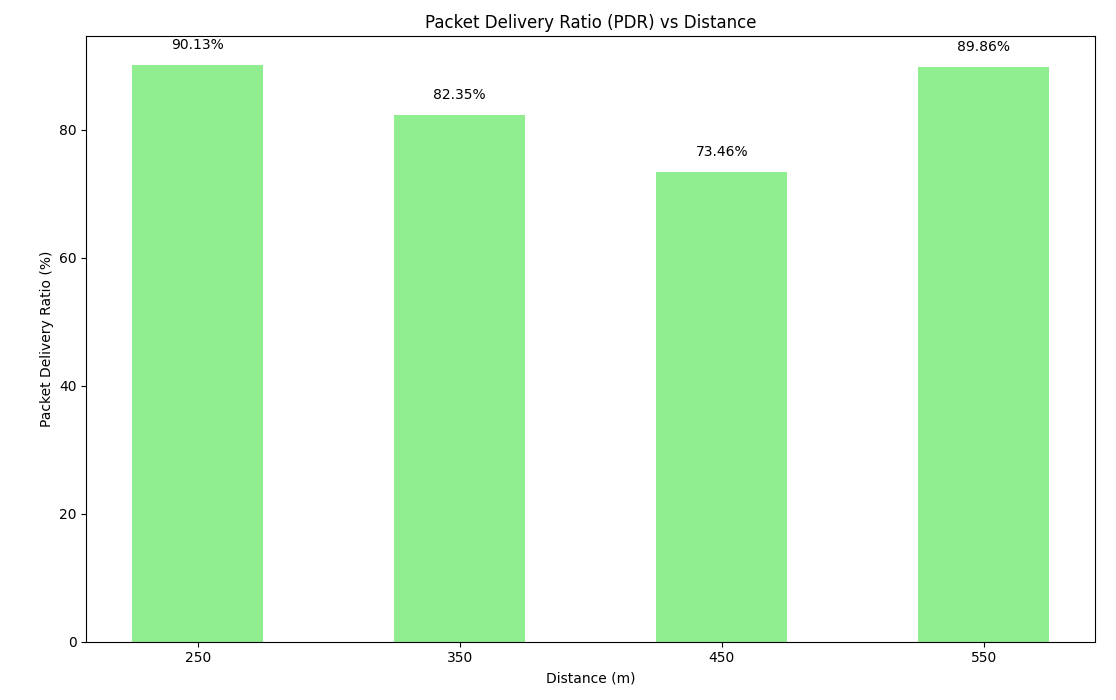
\includegraphics[width=0.8\textwidth]{image/PDR.png}
    \caption{PDR for Normal AODV}
    \label{fig:rtt_normal_aodv}
\end{figure}
\begin{figure}[h!]
    \centering
    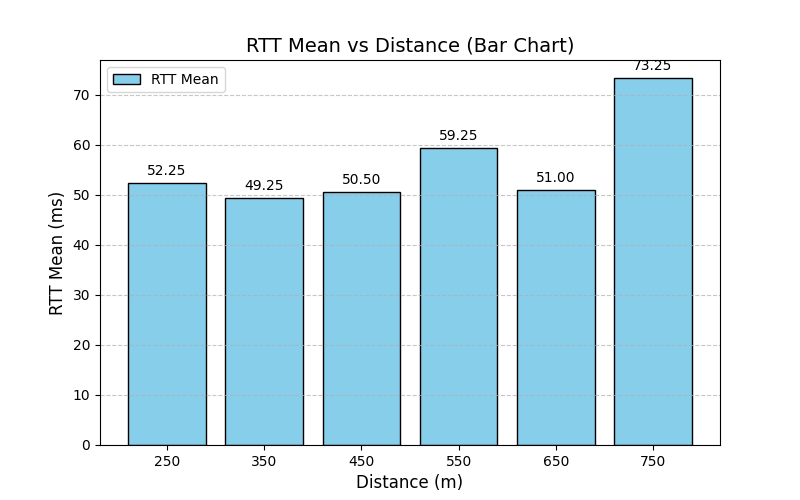
\includegraphics[width=0.8\textwidth]{image/RTT_2Hops.png}
    \caption{RTT for Normal AODV}
    \label{normal_aodv}
\end{figure}
\clearpage
\chapter{CSV DATA Extended AODV}
\begin{longtable}{llllll}
\caption{Sender Data} \label{tab:sender} \\
\toprule
Timestamp & ID & packet Type & Action & Bytes & Packet Count \\
\midrule
2025-01-03 21:25:22.493 & 73 & RREQ & sent & 36 & 1 \\
2025-01-03 21:25:37.524 & 8 & RELREQ & broadcasted & 32 & 1 \\
2025-01-03 21:25:37.581 & 8 & RELREP & rec & 48 & 1 \\
2025-01-03 21:25:37.589 & 8 & RELREP & rec & 48 & 1 \\
2025-01-03 21:26:07.642 & _ & data & send & 20 & 1 \\
2025-01-03 21:26:15.308 & 22 & RREQ & sent & 36 & 1 \\
2025-01-03 21:26:30.340 & 95 & RELREQ & broadcasted & 32 & 1 \\
2025-01-03 21:26:30.398 & 95 & RELREP & rec & 48 & 1 \\
2025-01-03 21:26:30.466 & 95 & RELREP & rec & 48 & 1 \\
2025-01-03 21:27:00.597 & _ & data & send & 20 & 1 \\
2025-01-03 21:27:09.742 & 25 & RREQ & sent & 36 & 1 \\
2025-01-03 21:27:24.776 & 33 & RELREQ & broadcasted & 32 & 1 \\
2025-01-03 21:27:24.830 & 33 & RELREP & rec & 48 & 1 \\
2025-01-03 21:27:24.886 & 33 & RELREP & rec & 48 & 1 \\
2025-01-03 21:27:54.990 & _ & data & send & 20 & 1 \\
2025-01-03 21:28:00.409 & 67 & RREQ & sent & 36 & 1 \\
2025-01-03 21:28:15.444 & 51 & RELREQ & broadcasted & 32 & 1 \\
2025-01-03 21:28:15.495 & 51 & RELREP & rec & 48 & 1 \\
2025-01-03 21:28:15.556 & 51 & RELREP & rec & 48 & 1 \\
2025-01-03 21:28:45.677 & _ & data & send & 20 & 1 \\
2025-01-03 21:29:06.906 & 30 & RREQ & sent & 36 & 1 \\
2025-01-03 21:29:21.937 & 44 & RELREQ & broadcasted & 32 & 1 \\
2025-01-03 21:29:21.999 & 44 & RELREP & rec & 48 & 1 \\
2025-01-03 21:29:22.053 & 44 & RELREP & rec & 48 & 1 \\
2025-01-03 21:29:52.141 & _ & data & send & 20 & 1 \\
2025-01-03 21:32:03.198 & 27 & RREQ & sent & 36 & 1 \\
2025-01-03 21:32:18.233 & 11 & RELREQ & broadcasted & 32 & 1 \\
2025-01-03 21:32:18.296 & 11 & RELREP & rec & 48 & 1 \\
2025-01-03 21:32:18.357 & 11 & RELREP & rec & 48 & 1 \\
2025-01-03 21:32:48.448 & _ & data & send & 20 & 1 \\
2025-01-03 21:32:52.090 & 49 & RREQ & sent & 36 & 1 \\
2025-01-03 21:33:07.126 & 58 & RELREQ & broadcasted & 32 & 1 \\
2025-01-03 21:33:07.189 & 58 & RELREP & rec & 48 & 1 \\
2025-01-03 21:33:07.245 & 58 & RELREP & rec & 48 & 1 \\
2025-01-03 21:33:37.375 & _ & data & send & 20 & 1 \\
2025-01-03 21:33:51.378 & 65 & RREQ & sent & 36 & 1 \\
2025-01-03 21:34:06.402 & 21 & RELREQ & broadcasted & 32 & 1 \\
2025-01-03 21:34:06.473 & 21 & RELREP & rec & 48 & 1 \\
2025-01-03 21:34:06.529 & 21 & RELREP & rec & 48 & 1 \\
2025-01-03 21:34:36.654 & _ & data & send & 20 & 1 \\
2025-01-03 21:34:41.309 & 64 & RREQ & sent & 36 & 1 \\
2025-01-03 21:34:56.345 & 31 & RELREQ & broadcasted & 32 & 1 \\
2025-01-03 21:34:56.396 & 31 & RELREP & rec & 48 & 1 \\
2025-01-03 21:34:56.457 & 31 & RELREP & rec & 48 & 1 \\
2025-01-03 21:35:26.558 & _ & data & send & 20 & 1 \\
2025-01-03 21:35:37.335 & 9 & RREQ & sent & 36 & 1 \\
2025-01-03 21:35:52.368 & 66 & RELREQ & broadcasted & 32 & 1 \\
2025-01-03 21:35:52.427 & 66 & RELREP & rec & 48 & 1 \\
2025-01-03 21:35:52.465 & 66 & RELREP & rec & 48 & 1 \\
2025-01-03 21:36:22.573 & _ & data & send & 20 & 1 \\
2025-01-03 21:38:31.020 & 22 & RREQ & sent & 36 & 1 \\
2025-01-03 21:38:46.056 & 93 & RELREQ & broadcasted & 32 & 1 \\
2025-01-03 21:38:46.126 & 93 & RELREP & rec & 48 & 1 \\
2025-01-03 21:38:46.183 & 93 & RELREP & rec & 48 & 1 \\
2025-01-03 21:39:16.299 & _ & data & send & 20 & 1 \\
2025-01-03 21:39:49.382 & 57 & RREQ & sent & 36 & 1 \\
2025-01-03 21:40:04.416 & 50 & RELREQ & broadcasted & 32 & 1 \\
2025-01-03 21:40:04.480 & 50 & RELREP & rec & 48 & 1 \\
2025-01-03 21:40:04.553 & 50 & RELREP & rec & 48 & 1 \\
2025-01-03 21:40:34.639 & _ & data & send & 20 & 1 \\
2025-01-03 21:40:46.992 & 37 & RREQ & sent & 36 & 1 \\
2025-01-03 21:41:02.028 & 35 & RELREQ & broadcasted & 32 & 1 \\
2025-01-03 21:41:02.097 & 35 & RELREP & rec & 48 & 1 \\
2025-01-03 21:41:02.161 & 35 & RELREP & rec & 48 & 1 \\
2025-01-03 21:41:32.267 & _ & data & send & 20 & 1 \\
2025-01-03 21:41:47.589 & 76 & RREQ & sent & 36 & 1 \\
2025-01-03 21:42:02.624 & 44 & RELREQ & broadcasted & 32 & 1 \\
2025-01-03 21:42:02.672 & 44 & RELREP & rec & 48 & 1 \\
2025-01-03 21:42:02.673 & 44 & RELREP & rec & 48 & 1 \\
2025-01-03 21:42:32.764 & _ & data & send & 20 & 1 \\
2025-01-03 21:42:36.592 & 44 & RREQ & sent & 36 & 1 \\
2025-01-03 21:42:51.629 & 6 & RELREQ & broadcasted & 32 & 1 \\
2025-01-03 21:42:51.688 & 6 & RELREP & rec & 48 & 1 \\
2025-01-03 21:42:51.755 & 6 & RELREP & rec & 48 & 1 \\
2025-01-03 21:43:21.871 & _ & data & send & 20 & 1 \\
2025-01-03 21:46:42.021 & 86 & RREQ & sent & 36 & 1 \\
2025-01-03 21:46:57.056 & 27 & RELREQ & broadcasted & 32 & 1 \\
2025-01-03 21:46:57.111 & 27 & RELREP & rec & 48 & 1 \\
2025-01-03 21:46:57.173 & 27 & RELREP & rec & 48 & 1 \\
2025-01-03 21:47:27.252 & _ & data & send & 20 & 1 \\
2025-01-03 21:47:31.591 & 99 & RREQ & sent & 36 & 1 \\
2025-01-03 21:47:46.626 & 43 & RELREQ & broadcasted & 32 & 1 \\
2025-01-03 21:47:46.688 & 43 & RELREP & rec & 48 & 1 \\
2025-01-03 21:47:46.770 & 43 & RELREP & rec & 48 & 1 \\
2025-01-03 21:48:16.893 & _ & data & send & 20 & 1 \\
2025-01-03 21:48:21.715 & 88 & RREQ & sent & 36 & 1 \\
2025-01-03 21:48:36.743 & 80 & RELREQ & broadcasted & 32 & 1 \\
2025-01-03 21:48:36.799 & 80 & RELREP & rec & 48 & 1 \\
2025-01-03 21:48:36.856 & 80 & RELREP & rec & 48 & 1 \\
2025-01-03 21:49:06.952 & _ & data & send & 20 & 1 \\
\bottomrule
\end{longtable}
\clearpage

\section{Extended AODV}
\begin{figure}[h!]
    \centering
    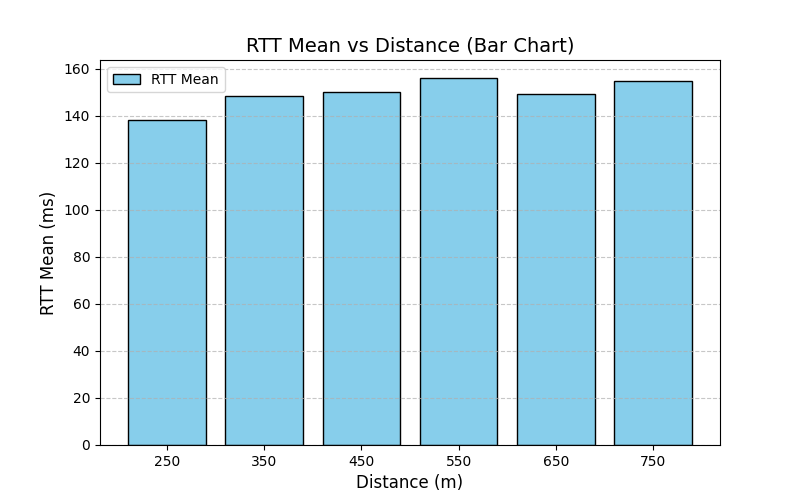
\includegraphics[width=0.8\textwidth]{image/RTT_extended.png}
    \caption{RTT for Extended AODV}
    \label{fig:rtt_extended_aodv}
\end{figure}
\begin{figure}[h!]
    \centering
    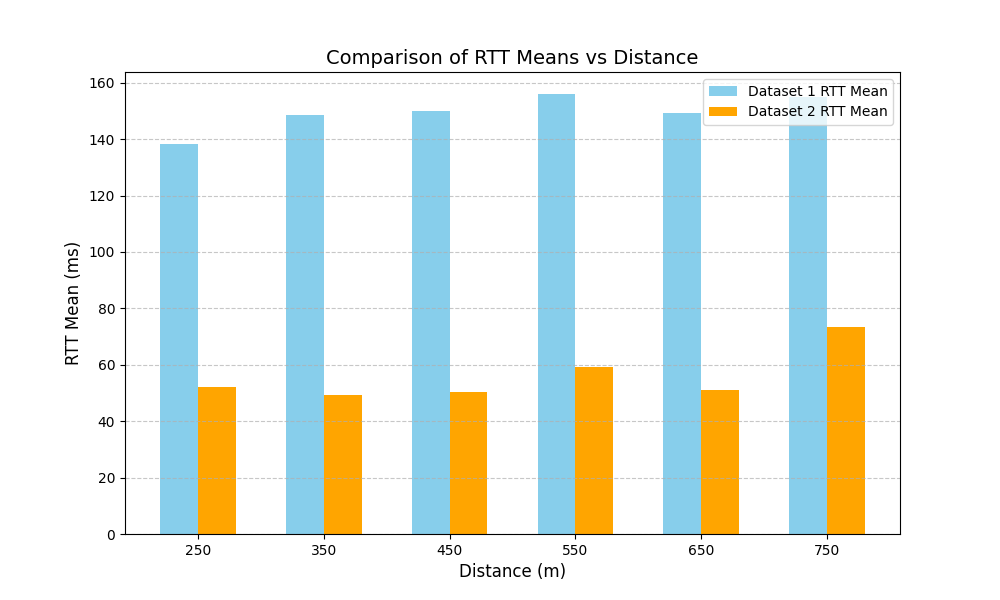
\includegraphics[width=0.8\textwidth]{image/RTTDiffernce.png}
    \caption{Normal AODV vs Extended AODV}
    \label{fig:rtt_extended_aodv}
\end{figure}

\chapter{Underwater Data Forwarding}
\section{Underwater Data Forwarding Latency}
\vspace{3cm}
\begin{figure}[h!]
    \centering
    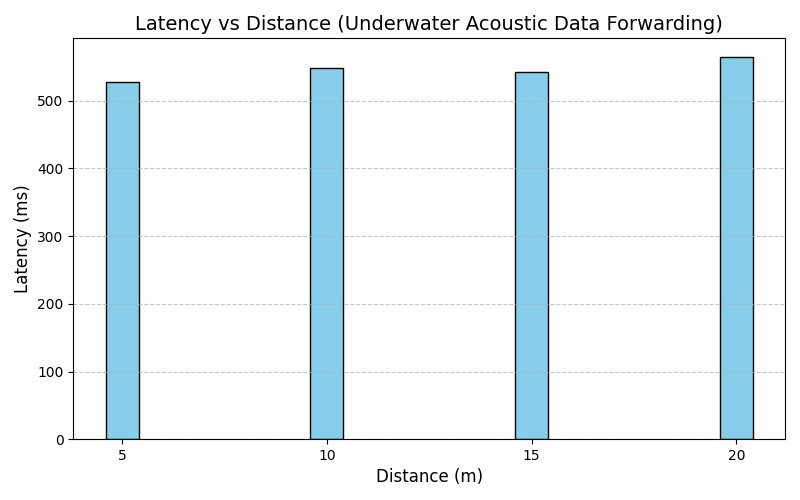
\includegraphics[width=0.9\textwidth]{image/Figure_1.png}
    \caption{Data Forwarding Latency}
    \label{fig:rtt_extended_aodv}
\end{figure}
\cleardoublepage

\listofabbreviations
\newenvironment{abbreviations}{
  \begin{description}
    \setlength{\itemsep}{0.5em} % Adjust space between items
}{\end{description}}
\begin{abbreviations}
    \item [AODV] ............................ Ad-hoc On-demand Distance Vector
    \item [B.A.T.M.A.N.] ............................ Better Approach to Mobile Ad hoc Networking 
    \item [DBR] ............................ Depth-Based Routing
    \item [DSR] ............................ Dynamic Source Routing
    \item [MDO] ............................ Multi-Domain Operations
    \item [MANET] ............................ Mobile Ad Hoc Network
    \item [OLSR] ............................ Optimized Link State Routing
    \item [PDR] ............................ Packet Delivery Ratio 
    \item [RREQ] ............................ Route Request 
    \item [RREP] ............................ Route Reply
    \item [RelReq] ............................ Relay Request 
    \item [RelRep] ............................ Relay Reply 
    \item [Raspi] ............................ Raspberry pi
    \item [RTT] ............................ Round Trip Time
    \item [S2C] ............................ Sweep-Spread Carrier
    \item [UAV] ............................ Unmanned Aerial Vehicle
    \item [USV] ............................ Unmanned Surface Vehicle
    \item [UUV] ............................ Unmanned Underwater Vehicle
    \item [UxV] ............................ Unmanned Vehicle
    \item [UANET] ............................ Underwater Ad Hoc Network
    \item [VBF] ............................ Vector-Based Forwarding
    
    
\end{abbreviations}
\clearpage

\listoffigures
\clearpage

\listoftables
\clearpage

\printbibliography

\end{document}
